\documentclass[
    11pt,
    oneside,
    doublespace
]{tudat}
%\usepackage{subfig}
\usepackage[
    list=false % remove from list of figures
]{subcaption}
\usepackage{parskip}

%\usepackage[%
%    font={small,sf},
%    labelfont=bf,
%    format=hang,
%    format=plain,
%    margin=0pt,
%    width=0.8\textwidth,
%]{caption}
%\usepackage[list=true]{subcaption}
%---------------------------
% Paper size
%---------------------------
\usepackage{geometry}
\geometry{
    paper=a4paper,  % Change to letterpaper for US letter
    inner=2.5cm,    % Inner margin
    outer=2.5cm,    % Outer margin
% 	bindingoffset=.5cm, % Binding offset
    top=2.5cm,      % Top margin
    bottom=2.5cm,   % Bottom margin
% 	showframe,      % Uncomment to show the precise text area
}

%---------------------------
% Acronyms (acro.tex)
%---------------------------
%\usepackage{acro}
%\acsetup{
%    first-style=short,
%    make-links = true,
%}
\usepackage{longtable}
\usepackage[acronym, order=letter]{glossaries}


%---------------------------
% Math
%---------------------------
% bold math symbols
\usepackage{bm}
\usepackage{amsfonts}
\usepackage{mathtools}

%---------------------------
% Physics
%---------------------------
% Enables partial derivatives using: \dv{a}{t}
\usepackage{physics}
%\usepackage{xcolor}

%---------------------------
% Figures
%---------------------------
\usepackage{import}   % For use with SVG's from GIMP (pdf_tex)
\let\savediv\div
\let\div\relax
\usepackage{mathabx}  % For use with SVG's from GIMP (pdf_tex)
\let\div\savedev

\usepackage[labelfont=bf]{caption}
%---------------------------
% TikZ
%---------------------------
\usepackage{tikz}
\usetikzlibrary{
    positioning,
    arrows.meta,
    calc,
    decorations.pathreplacing,
    decorations.text,
    bending,
    matrix}
\usetikzlibrary{matrix}
%\usetikzlibrary{decorations.pathreplacing}    % for TikZ braces
%\usetikzlibrary{positioning}                  % for TikZ relative positioning

%---------------------------
% Appendices
%---------------------------
\usepackage[toc]{appendix}
%\newcommand*{\Appendixautorefname}{Appendix}
\def\appendixautorefname{Appendix}

%---------------------------

% Plots
%---------------------------
\usepackage{pgfplots}
\pgfplotsset{every axis/.append style={tick label style={/pgf/number format/fixed},font=\scriptsize,ylabel near ticks,xlabel near ticks,grid=major}}
\pgfplotsset{compat=1.16}


%$ error-capacity plot

%\usepackage[dvipsnames]{xcolor}
%\usepackage{pgfplots}
\usepackage{sansmath}
%\usepackage[style=nature,backend=bibtex]{biblatex}
%\addbibresource{bib.bib}
%---------------------------
% Bibliography
%---------------------------

%
% \usepackage[nottoc]{tocbibind} % Include in TOC

\usepackage[
    natbib=true,
    backend=bibtex,
%    sorting=anyvt,
    url=true,
    style=nature,
    doi=true]{biblatex}
\bibliography{library}
\addbibresource{library}
%%\usepackage[nottoc]{tocbibind} % Include in TOC


%%%%%%%%%%%%%%%%%%%%%%%%%%%%%%%%%%%%%%%%%%%%%%%%%%%%%%%%%%%%%%%%%%%%%%%%%%%%%%%
% COVER PAGE
%%%%%%%%%%%%%%%%%%%%%%%%%%%%%%%%%%%%%%%%%%%%%%%%%%%%%%%%%%%%%%%%%%%%%%%%%%%%%%%
\usepackage{hyperref}


%%%%%%%%%%%%%%%%%%%%%%%%%%%%%%%%%%%%%%%%%%%%%%%%%%%%%%%%%%%%%%%%%%%%%%%%%%%%%%%
% PACKAGES
%%%%%%%%%%%%%%%%%%%%%%%%%%%%%%%%%%%%%%%%%%%%%%%%%%%%%%%%%%%%%%%%%%%%%%%%%%%%%%%
\usepackage[utf8]{inputenc}
\usepackage{textcomp}

% paragraph linbreaks


\usepackage{mathtools}
%\usepackage{tikz}

% for braces

%\usepackage{graphicx}
%\usepackage{amsmath}
%\usepackage[version=4]{mhchem}
%\usepackage{siunitx}
%\usepackage{longtable,tabularx}
%\setlength\LTleft{0pt}


%added after

% stop caption being bold with \textmd{medium/regular}
%\usepackage[font=bf]{caption}
\usepackage[
%    natbib=true,
    backend=bibtex,
    sorting=anyvt,
    url=true,
    style=nature,
    doi=true]{biblatex}

\addbibresource{sample.bib}
\bibliography{sample}

%%%%%%%%%%%%%%%%%%%%%%%%%%%%%%%%%%%%%%%%%%%%%%%%%%%%%%%%%%%%%%%%%%%%%%%%%%%%%%%
% DOCUMENT
%%%%%%%%%%%%%%%%%%%%%%%%%%%%%%%%%%%%%%%%%%%%%%%%%%%%%%%%%%%%%%%%%%%%%%%%%%%%%%%
\begin{document}

    \pagenumbering{gobble}

    %% Roman numerals
%    \makecover

    \frontmatter % Use roman page numbering style

    % \noindent(Nomenclature entries should have the units identified)

% {\renewcommand\arraystretch{1.0}
% \noindent\begin{longtable*}{@{}l @{\quad=\quad} l@{}}
% $A$  & amplitude of oscillation \\
% $a$ &    cylinder diameter \\
% $C_p$& pressure coefficient \\
% $Cx$ & force coefficient in the \textit{x} direction \\
% $Cy$ & force coefficient in the \textit{y} direction \\
% c   & chord \\
% d$t$ & time step \\
% $Fx$ & $X$ component of the resultant pressure force acting on the vehicle \\
% $Fy$ & $Y$ component of the resultant pressure force acting on the vehicle \\
% $f, g$   & generic functions \\
% $h$  & height \\
% $i$  & time index during navigation \\
% $j$  & waypoint index \\
% $K$  & trailing-edge (TE) nondimensional angular deflection rate\\
% $\Theta$ & boundary-layer momentum thickness\\
% $\rho$ & density\\
% \multicolumn{2}{@{}l}{Subscripts}\\
% cg & center of gravity\\
% $G$ & generator body\\
% iso	& waypoint index
% \end{longtable*}}
%

    \listoffigures
    \listoftables

    \newpage

    \setcounter{tocdepth}{2} % Set TOC to display up to subsections
    \tableofcontents

    \mainmatter % Begin numeric (1,2,3...) page numbering

    \chapter{Introduction}

One component of paramount importance for the preservation of all known life in
the observable universe, is humanities capabilities to detect, track, and
characterize \glspl{NEO}. Two of these aspects: \textit{detection} and
\textit{characterization}, exhibit significant potential returns in our
continued progression towards their complete intelligence-based automation.

A significant failure in automated \textit{detection} was demonstrated by anb
event which left scientists {``stunned [and in] true shock"}~\cite{chiu_2019}. A
small body, later named ``2019 OK",  was discovered only \textbf{24 hours} prior
to its closest approach in 2019 when it was approximately 0.01 AU ($\approx$1.5
million kilometers) away from Earth with an apparent magnitude of
14.7~\cite{IAU2019OK} (a measure of relative brightness visible with a 203 mm
telescope aperture~\cite[p.~24]{North2014}). It passed Earth at a distance of
$\approx$70,000 km, less than one-fifth of the distance to the Moon. The % closest approach or flyby
 object's size was estimated to be between 57-130 m in
diameter~\cite{NASA2019}. The mass of a small body is often estimated by
observing its gravitational interaction with another object, such as another
small body during their close encounter with one another. Without these
observations the mass may not be estimated, however, given the characteristics
of other known small bodies, the effect of the impact of an Asteroid in diameter
range of 2019 OK, would yield between 10-300 megatons of explosive force
\cite{Cellino1999, Rumpf2017}. For reference, 1 megaton is equivalent to 1
million tons of TNT. A next widely known reference: approximately 5 megatons of
energy were released by tsunami waves following the ``2004 Indian Ocean
earthquake" (a.k.a. the ``Sumatra-Andaman earthquake") \cite{Nirupama2006} which
killed at least 225,000 people across a dozen countries. Finally, our largest


reference in the magnitude of explosive yield, the ``Tsar Bomba". This was the
most powerful nuclear weapon ever created by humanity, with an explosive yield
of 50 megatons~\cite{Khan2020} (theoretical yield of 100 megatons),
approximately 1300 times the \textbf{combined yield} of the prominent historical
devices by the names of ``Little Boy" and ``Fat Man", which were nuclear bombs
fueled by highly enriched uranium and dropped on Hiroshima and Nagasaki
respectively, bringing an end to World War II~\cite{osti_1489669}.
%It is in our
%best interest to remember our encounters with calamity throughout history, so
%that we may attempt to foresee the true consequences that an impact event would
%have on Earth, and ultimately preserve the future of humanity.
There is a subsequent consensus amongst scientists on the cause of the failure:
objects approaching in some directions of the sky towards Earth, can exhibit a
slow apparent motion. In the case of similar geometry to "2019 OK", the apparent
motion of the small bodies were shown to have been as low as 0.1 degrees per
day~\cite{Wainscoat2022}.

The requirements imposed on the timely characterization of an asteroid, in the
case of a small


\cite{Marks2022}


There have been many missions to small celestial bodies pursued by all humanity
in our drive to better understand the formation of the Solar System and the
conditions in the early solar nebula. The term \textit{small body} refers to any
celestial objects which avoided accretion by the Sun, a major planet, or their
largest moons. The major categories of scientific questions, for which
small body exploration bears the promise of answers, are ones addressing
\textit{the conditions of the early solar nebular} and \textit{planetesimal
formation}~\cite{Davidsson2021}.


% https://ssd.jpl.nasa.gov/tools/sbdb_lookup.html#/?sstr=3843336 database of small bodies from JPL.
% https://cneos.jpl.nasa.gov/nda/overview.html cool NASA app on NEO Deflection calculations.

%
%\begin{fancyquotes}
%    The sciences do not try to explain, they hardly even try to interpret, they
%    mainly make models. By a model is meant a mathematical construct which, with
%    the addition of certain verbal interpretations, describes observed
%    phenomena. The justification of such a mathematical construct is solely and
%    precisely that it is expected to work - that is correctly to describe
%    phenomena from a reasonably wide area. Furthermore, it must satisfy certain
%    aesthetic criteria - that is, in relation to how much it describes, it must
%    be rather simple. - John von Neumann
%\end{fancyquotes}

\section{Brief History of Spacecraft Missions to Small Celestial Bodies}

There have been many missions to small celestial bodies pursued by mankind in
our drive to better understand the formation of the Solar System and the
conditions in the early solar nebula. The term \textit{small body} refers to any
celestial objects which avoided accretion by the Sun, a major planet, or their
largest moons. The major categories of scientific questions which, for which
small body exploration bears promising of answering, are ones addressing
\textit{the conditions of the early solar nebular} and \textit{planetisimanl
formation}~\cite{Davidsson2021}.
    %%%%%%%%%%%%%%%%%%%%%%%%%%%%%%%%%%%%%%%%%%%%%%%%%%%%%%%%%%%%%%%%%%%%%%%%%%%%%%%%
\chapter{Orbital Mechanics}
%%%%%%%%%%%%%%%%%%%%%%%%%%%%%%%%%%%%%%%%%%%%%%%%%%%%%%%%%%%%%%%%%%%%%%%%%%%%%%%%

At the core of astrodynamics, the two-body restricted problem describes the
motion of a secondary body of negligible mass orbiting a central body, with no
other sources of acceleration in the system. This problem is described by
Newton's equation of planetary motion

\begin{equation}
    \ddot{\mathbf{r}}=-\frac{\mu}{r^3}\mathbf{r},
    \label{eq:newtons_equation_planetary}
\end{equation}
\begin{equation*}
    \begin{aligned}
        \textrm{where }
        \mathbf{r}&=\textrm{the Cartesian, a.k.a. the rectangular coordinate position vector relative to the central body,}\\
        \mu&=GM=\textrm{the gravitational parameter of the central body,}\\
        G&=\textrm{the universal gravitational constant,}\\
        M&=\textrm{the mass of the central body.}
    \end{aligned}
\end{equation*}

%%%%%%%%%%%%%%%%%%%%%%%%%%%%%%%%%%%%%%%%%%%%%%%%%%%%%%%%%%%%%%%%%%%%%%%%%%%%%%%%
\section{Reference Frames}
%%%%%%%%%%%%%%%%%%%%%%%%%%%%%%%%%%%%%%%%%%%%%%%%%%%%%%%%%%%%%%%%%%%%%%%%%%%%%%%%

There are various categories of reference frames used within astrophysics and
astrodynamics. Some frames are \textit{outdated} in nature, but are however
still documented and commonly used to ensure the usability of historical
empirical data. This section will cover the generalised taxonomy of these
reference frames, with mention of common frames and where they fit within the
taxonomy.

\begin{figure}[h]
    \centering
    \def\svgwidth{0.75\linewidth}
    \import{graphics/}{ths_base_frame.pdf_tex}
    \caption{Definition of a right-handed reference frame.}
    \label{fig:frames_rh}
\end{figure}

Unless stated otherwise, one should assume that all orthogonal reference frames
used within astrodynamics are right-handed, defined by
$\mathbf{X}\cross{\mathbf{Y}}=\mathbf{Z}$ as illustrated in
\autoref{fig:frames_rh}. The contemporary reference systems used in astronomy
and astrophysics are defined International Astronomical Union (IAU). Due to the
long history of the field, there are many others outside of the IAU's
standardised frames which are still used for a multitude of reasons, one being
the need to ensure accessibility to older observations which were made in the
older alternative systems.

%%%%%%%%%%%%%%%%%%%%%%%%%%%%%%%%%%%%%%%%%%%%%%%%%%%%%%%%%%%%%%%%%%%%%%%%%%%%%%%%
\subsection{Earth-centred inertial (ECI)\label{ssec:frame_intertial}}
%%%%%%%%%%%%%%%%%%%%%%%%%%%%%%%%%%%%%%%%%%%%%%%%%%%%%%%%%%%%%%%%%%%%%%%%%%%%%%%%

\begin{figure}[h]
    \centering
    \def\svgwidth{0.75\linewidth}
    % \input{graphics/drawing2.pdf_tex}
    \import{graphics/}{ths_j2000.pdf_tex}
    \caption{Definition of the J2000 Earth-centred inertial (ECI) frame.}
    \label{fig:my_label}
\end{figure}

%%%%%%%%%%%%%%%%%%%%%%%%%%%%%%%%%%%%%%%%%%%%%%%%%%%%%%%%%%%%%%%%%%%%%%%%%%%%%%%%
\subsection{Inertial\label{ssec:frame_intertial}}
%%%%%%%%%%%%%%%%%%%%%%%%%%%%%%%%%%%%%%%%%%%%%%%%%%%%%%%%%%%%%%%%%%%%%%%%%%%%%%%%

An inertial reference frame is a non-rotating frame with a non-accelerating
origin. All inertial reference frames are in a state of constant rectilinear
motion with respect to one another. Strictly speaking, "inertial" is used in
place of "quasi-inertial", as no reference frame we use is truly
non-accelerating. This approximation is accepted due to the near negligible
acceleration these frames' origins. From this point forwards, "inertial" will be
used in place of "quasi-inertial". There are two frames which are used in
astrophysics as the lowest level in the hierarchy, namely J2000 (a.k.a. EME2000)
and the International Celestial Reference Frame (ICRF).

\textcolor{red}{Include illustrations for the J2000 (EMEJ2000) frame and the
origin of its definition. Explain how ICRS was an interaction on this frame.
Explain also how J2000 is related to the Earth-centered inertial (ECI) reference
frame, leading to the next subsection on BCI.}

%%%%%%%%%%%%%%%%%%%%%%%%%%%%%%%%%%%%%%%%%%%%%%%%%%%%%%%%%%%%%%%%%%%%%%%%%%%%%%%%
\subsection{Body-centered inertial (BCI)}
%%%%%%%%%%%%%%%%%%%%%%%%%%%%%%%%%%%%%%%%%%%%%%%%%%%%%%%%%%%%%%%%%%%%%%%%%%%%%%%%

The Body-centered inertial (BCI) reference frames are frames which have their
origins at the center of mass of a body, the $Z_C$-axis is directed along the
(counter clockwise positive) spin-axis of the body, the $X_C$-axis passes
through the ascending node of the intersection between the ecliptic and the
equator of the body. The $Y_C$-axis then passes through the equatorial plane
perpendicular to $X_C$ and $Z_C$-axis to complete the rectangular coordinate
system.

\begin{figure}[!htp]
    \centering
    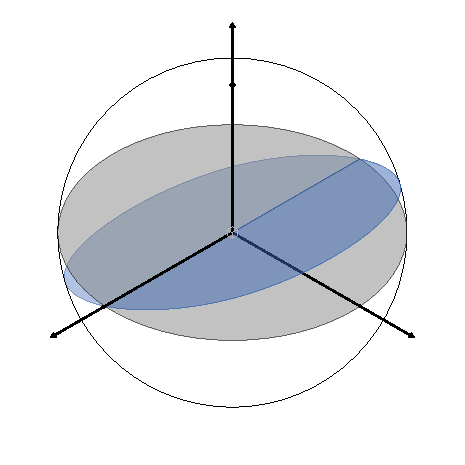
\includegraphics[width=0.4\linewidth]{graphics/test.pdf}
    \caption{Definition of a general Body-centered inertial (BCI) reference frame.}
    \label{fig:bci}
\end{figure}

\begin{figure}[h]
    \centering
    \def\svgwidth{0.4\linewidth}
    % \input{graphics/drawing2.pdf_tex}
    \import{graphics/}{test.pdf_tex}
    \caption{Definition of a general Body-centered inertial (BCI) reference frame.}
    \label{fig:my_label}
\end{figure}

%%%%%%%%%%%%%%%%%%%%%%%%%%%%%%%%%%%%%%%%%%%%%%%%%%%%%%%%%%%%%%%%%%%%%%%%%%%%%%%%
\subsection{Body-centered body-fixed (BCBF)\label{ssec:frame_bcbf}}
%%%%%%%%%%%%%%%%%%%%%%%%%%%%%%%%%%%%%%%%%%%%%%%%%%%%%%%%%%%%%%%%%%%%%%%%%%%%%%%%

The body-centered body-fixed (BCBF) reference frames are frames which have their
origins at the center of mass of a body, the $Z_F$-axis is directed along
(counter clockwise positive) spin-axis of the body. The $X_F$-axis passes
through the reference meridian of the body, which is at an angle of
$\Omega_t{t_0}$ from the ascending node of the intersection between the ecliptic
and the equator of the body. The $Y_F$-axis then passes through the equatorial
plane perpendicular to $X_F$ and $Z_F$.

\begin{figure}[!htp]
    \centering
    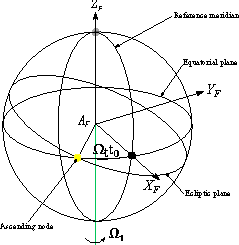
\includegraphics[width=0.35\linewidth]{graphics/bcbf.pdf}
    \caption{
        Definition of a general Body-centered body-fixed (BCBF) reference frame.
    }
    \label{fig:bci}
\end{figure}


\begin{equation}
    W = W_0 + \dot{W}d
    \label{eq:ephem_prime_meridian}
\end{equation}
\begin{equation*}
    \begin{aligned}
        \textrm{where, }
        W &= \textrm{the ephemeris position of the prime meridian} \\
        W_0 &= \textrm{the value of W at J2000.0 (occasionally some other epoch),} \\
        d &= \textrm{interval in days from the standard epoch.}
    \end{aligned}
\end{equation*}

\begin{equation}
    \mathbf{R}^{I/B}=\mathbf{R}_z(W)\mathbf{R}_x(\pi/2-\delta_0)\mathbf{R}_z(\pi/2-\alpha_0)
    \label{eq:bci_transformation}
\end{equation}
\begin{equation*}
    \begin{aligned}
        \textrm{where, }
        \mathbf{R}_{x,y,z}(\phi) &= \textrm{transformation matrix for a rotation of $\phi$ radians about the respective axis (\autoref{appendix:rotational_transformations}),}\\
        \alpha_0, \delta_0 &= \textrm{ICRF equatorial coordinates at epoch J2000.0} \\
    \end{aligned}
\end{equation*}

%%%%%%%%%%%%%%%%%%%%%%%%%%%%%%%%%%%%%%%%%%%%%%%%%%%%%%%%%%%%%%%%%%%%%%%%%%%%%%%%
\subsection{Radial tangential normal (RTN)\label{ssec:frame_rtn}\label{ssec:frame_rsw}}
%%%%%%%%%%%%%%%%%%%%%%%%%%%%%%%%%%%%%%%%%%%%%%%%%%%%%%%%%%%%%%%%%%%%%%%%%%%%%%%%

The radial tangential normal frame (RTN), a.k.a. the radial (R), along-track (S)
and cross-track (W) frame (RSW), is a dynamic frame with an orbiting spacecraft
at the centre of the frame. The frame is time dependent and based on the
two-body restricted problem problem with the R-component determined by the
current unit-vector of position $\hat{r}$, the T-component by the unit vector of
velocity $\hat{v}$, and the N-component by their the cross product of the two,
the specific angular momentum vector $\hat{r}\cross{\hat{v}}=\hat{h}$. This
frame is commonly used for relative motion of spacecraft in a rendezvous
segment.

\begin{equation}
    \mathbf{R}^{I/RSW}= \bigg[\hat{\mathbf{r}}_{B/S}\; \hat{\mathbf{v}}_{B/S}\; \hat{\mathbf{h}}_{B/S} \bigg]
\end{equation}
\begin{equation*}
    \begin{aligned}
        \textrm{where, }
        \hat{\mathbf{r}}_{B/S} &= \textrm{the position of the spacecraft with respect to the body,}\\
        \hat{\mathbf{v}}_{B/S} &= \textrm{the velocity of the spacecraft with respect to the body,}\\
        \hat{\mathbf{h}}_{B/S} &= \textrm{the specific angular momentum of the spacecraft with respect to the body,}\\
    \end{aligned}
\end{equation*}

%%%%%%%%%%%%%%%%%%%%%%%%%%%%%%%%%%%%%%%%%%%%%%%%%%%%%%%%%%%%%%%%%%%%%%%%%%%%%%%%
\section{Orbital Elements}
%%%%%%%%%%%%%%%%%%%%%%%%%%%%%%%%%%%%%%%%%%%%%%%%%%%%%%%%%%%%%%%%%%%%%%%%%%%%%%%%
Orbital elements are a set of parameters which uniquely define a Keplerian, or
two-body restricted orbit, around a given central body in the absence of any
external perturbations incurred in the system. This definition is given with
with respect to a plane of reference and a reference direction. Conversion
between any arbitrary pair of orbital elements of a given reference plane and
direction, requires only the central body's gravitational parameter $\mu$.

%%%%%%%%%%%%%%%%%%%%%%%%%%%%%%%%%%%%%%%%%%%%%%%%%%%%%%%%%%%%%%%%%%%%%%%%%%%%%%%%
\subsection{Cartesian}
%%%%%%%%%%%%%%%%%%%%%%%%%%%%%%%%%%%%%%%%%%%%%%%%%%%%%%%%%%%%%%%%%%%%%%%%%%%%%%%%
The Cartesian, a.k.a. the rectangular orbital elements are the concatenation of
the position and velocity vectors in the respectively named coordinate system
relative to the central body,

\begin{equation}
    \textrm{\OE}_C=
    \begin{bmatrix}
        \mathbf{r}^T &
        \mathbf{v}^T &
    \end{bmatrix}^T
    =
    \begin{bmatrix}
        r_x &
        r_y &
        r_z &
        v_x &
        v_y &
        v_z &
    \end{bmatrix}^T,
\end{equation}

where all values are assumed as S.I. units, where not specified otherwise, in
further calculations involving the orbital elements.

%%%%%%%%%%%%%%%%%%%%%%%%%%%%%%%%%%%%%%%%%%%%%%%%%%%%%%%%%%%%%%%%%%%%%%%%%%%%%%%%
\subsection{Keplerian}
%%%%%%%%%%%%%%%%%%%%%%%%%%%%%%%%%%%%%%%%%%%%%%%%%%%%%%%%%%%%%%%%%%%%%%%%%%%%%%%%
The Keplerian, a.k.a. the classical orbital elements are the

\begin{equation}
    \textrm{\OE}_K=
    \begin{bmatrix}
        a &
        e &
        i &
        \Omega &
        \omega &
        \theta &
    \end{bmatrix}^T,
\end{equation}

%%%%%%%%%%%%%%%%%%%%%%%%%%%%%%%%%%%%%%%%%%%%%%%%%%%%%%%%%%%%%%%%%%%%%%%%%%%%%%%%
\subsection{Modified Equinoctial}
%%%%%%%%%%%%%%%%%%%%%%%%%%%%%%%%%%%%%%%%%%%%%%%%%%%%%%%%%%%%%%%%%%%%%%%%%%%%%%%%
The Keplerian, a.k.a. the classical orbital elements are the

\begin{equation}
    \textrm{\OE}_{ME}=
    \begin{bmatrix}
        p &
        f &
        g &
        h &
        k &
        L
    \end{bmatrix}^T,
\end{equation}

\begin{equation}
    \begin{aligned}
        p=&a(1-e^2)\\
        f=&e\cos{(\omega+\Omega)}\\
        g=&e\cos{(\omega+\Omega)}\\
        h=&\tan{(i/2)}\cos{\Omega}\\
        k=&\tan{(i/2)}\sin{\Omega}\\
        L=&\Omega+\omega+\theta\\
    \end{aligned}
\end{equation}

\cite{Equinoctial}

%%%%%%%%%%%%%%%%%%%%%%%%%%%%%%%%%%%%%%%%%%%%%%%%%%%%%%%%%%%%%%%%%%%%%%%%%%%%%%%%
\section{Preliminary Orbit Determination}
%%%%%%%%%%%%%%%%%%%%%%%%%%%%%%%%%%%%%%%%%%%%%%%%%%%%%%%%%%%%%%%%%%%%%%%%%%%%%%%%

%%%%%%%%%%%%%%%%%%%%%%%%%%%%%%%%%%%%%%%%%%%%%%%%%%%%%%%%%%%%%%%%%%%%%%%%%%%%%%%%
\subsection{Gibbs method}
%%%%%%%%%%%%%%%%%%%%%%%%%%%%%%%%%%%%%%%%%%%%%%%%%%%%%%%%%%%%%%%%%%%%%%%%%%%%%%%%

%%%%%%%%%%%%%%%%%%%%%%%%%%%%%%%%%%%%%%%%%%%%%%%%%%%%%%%%%%%%%%%%%%%%%%%%%%%%%%%%
\subsection{Lambert's problem}
%%%%%%%%%%%%%%%%%%%%%%%%%%%%%%%%%%%%%%%%%%%%%%%%%%%%%%%%%%%%%%%%%%%%%%%%%%%%%%%%

%%%%%%%%%%%%%%%%%%%%%%%%%%%%%%%%%%%%%%%%%%%%%%%%%%%%%%%%%%%%%%%%%%%%%%%%%%%%%%%%
\subsection{Gauss method}
%%%%%%%%%%%%%%%%%%%%%%%%%%%%%%%%%%%%%%%%%%%%%%%%%%%%%%%%%%%%%%%%%%%%%%%%%%%%%%%%

%%%%%%%%%%%%%%%%%%%%%%%%%%%%%%%%%%%%%%%%%%%%%%%%%%%%%%%%%%%%%%%%%%%%%%%%%%%%%%%%
\section{Orbital Perturbations}
%%%%%%%%%%%%%%%%%%%%%%%%%%%%%%%%%%%%%%%%%%%%%%%%%%%%%%%%%%%%%%%%%%%%%%%%%%%%%%%%
In order to account for perturbations such as a non-spherical body, atmospheric
drag, propulsive thrust, solar radiation pressure, and other celestial objects
outside the two-body formulation, \autoref{eq:newtons_equation_planetary} can be
rewritten as

\begin{equation}
    \ddot{\mathbf{r}}=\frac{\mu}{|\mathbf{r}|^3}\mathbf{r}+\mathbf{p},
    \label{eq:newtons_equation_planetary_with_p}
\end{equation}
where $\mathbf{p}$ is the net perturbative accelerations from all sources other than the spherically symmetric gravitational attraction between the two bodies.

%%%%%%%%%%%%%%%%%%%%%%%%%%%%%%%%%%%%%%%%%%%%%%%%%%%%%%%%%%%%%%%%%%%%%%%%%%%%%%%%
\subsection{Cowell's method}
%%%%%%%%%%%%%%%%%%%%%%%%%%%%%%%%%%%%%%%%%%%%%%%%%%%%%%%%%%%%%%%%%%%%%%%%%%%%%%%%

\begin{equation}
    \begin{aligned}
        \ddot{\mathbf{r}}=\dv{\dot{\mathbf{r}}}{t}=-\frac{\mu}{r^3}\mathbf{r} + \mathbf{p}
    \end{aligned}
\end{equation}

%%%%%%%%%%%%%%%%%%%%%%%%%%%%%%%%%%%%%%%%%%%%%%%%%%%%%%%%%%%%%%%%%%%%%%%%%%%%%%%%
\subsection{Encke's method}
%%%%%%%%%%%%%%%%%%%%%%%%%%%%%%%%%%%%%%%%%%%%%%%%%%%%%%%%%%%%%%%%%%%%%%%%%%%%%%%%

%%%%%%%%%%%%%%%%%%%%%%%%%%%%%%%%%%%%%%%%%%%%%%%%%%%%%%%%%%%%%%%%%%%%%%%%%%%%%%%%
\subsection{Variational Equations: Lagrange Planetary}
%%%%%%%%%%%%%%%%%%%%%%%%%%%%%%%%%%%%%%%%%%%%%%%%%%%%%%%%%%%%%%%%%%%%%%%%%%%%%%%%

\begin{equation}
    \begin{aligned}
        \dv{a}{t}&=-\frac{2a^2}{\mu}\pdv{R}{t_p}\\
        \dv{e}{t}&=-\frac{\sqrt{1-e^2}}{\sqrt{\mu{a}}e}\pdv{R}{a} + \frac{a(1-e^2)}{\mu{e}} \pdv{R}{t_p}\\
        \dv{t_p}{t}&=\frac{2a^2}{\mu}\pdv{R}{a}+\frac{a(1-e^2)}{\mu{e}}\pdv{R}{e}\\
        \dv{\Omega}{t}&=\frac{1}{\sqrt{\mu{a}(1-e^2)}\sin{i}}\pdv{R}{i}\\
        \dv{i}{t}&=\frac{1}{\sqrt{\mu{a(1-e^2)}}}\bigg(\frac{1}{\tan{i}}\pdv{R}{\omega}-\frac{1}{\sin{i}}\pdv{R}{\Omega}\bigg)\\
        \dv{\omega}{t}&=-\frac{1}{\sqrt{\mu{a}(1-e^2)\tan{i}}}\pdv{R}{i}+\frac{\sqrt{1-e^2}}{\sqrt{\mu{a}}e}\pdv{R}{e}
    \end{aligned}
\end{equation}

%%%%%%%%%%%%%%%%%%%%%%%%%%%%%%%%%%%%%%%%%%%%%%%%%%%%%%%%%%%%%%%%%%%%%%%%%%%%%%%%
\subsection{Variational Equations: Gauss}
%%%%%%%%%%%%%%%%%%%%%%%%%%%%%%%%%%%%%%%%%%%%%%%%%%%%%%%%%%%%%%%%%%%%%%%%%%%%%%%%

\begin{equation}
    \begin{aligned}
        \dv{a}{t}&=2\sqrt{\frac{a}{\mu}}\bigg(F_R\frac{ae}{\sqrt{1-e^2}}\sin{\theta}+F_S\frac{a^2\sqrt{1-e^2}}{a(1-e\cos{E})}\bigg)\\
        \dv{e}{t}&=\frac{h}{\mu}\sin{\theta}F_R+\frac{1}{\mu{h}}\bigg((h^2+\mu{r})\cos{\theta}+\mu{r}\bigg)F_S\\
        \dv{i}{t}&=\frac{r}{h}\cos{(\omega+\theta)}F_W\\
        \dv{\Omega}{t}&=\frac{r}{h\sin{i}}\sin{(\omega+\theta)}F_W\\
        \dv{\omega}{t}&=-\frac{1}{eh}\bigg(\frac{h^2}{\mu}\cos{\theta}F_R-(r+\frac{h^2}{\mu}\sin{\theta}F_S)\bigg)-\frac{r\sin{\omega+\theta}}{h\tan{i}}F_W\\
        \dv{\theta}{t}&=\frac{h}{r^2}+\frac{1}{eh}\bigg(\frac{h^2}{\mu}\cos{\theta}F_R-(r+\frac{h^2}{\mu})\sin{\theta}F_S\bigg)
    \end{aligned}
\end{equation}

\begin{equation}
    \begin{aligned}
        \dv{p}{t}&=\frac{2p}{w}\sqrt{\frac{p}{\mu}}F_R\\
        \dv{f}{t}&=\sqrt{\frac{p}{\mu}}\bigg(F_R\sin{L}+[(w+1)\cos{L}+f]\frac{F_T}{w}-(h\sin{L}-k\cos{L})\frac{gF_N}{w}\bigg)\\
        \dv{g}{t}&=\sqrt{\frac{p}{\mu}}\bigg(-F_R\cos{L}+[(w+1)\sin{L}+g]\frac{F_T}{w}-(h\sin{L}-k\cos{L})\frac{gF_N}{w}\bigg)\\
        \dv{h}{t}&=\sqrt{\frac{p}{\mu}}\frac{s^2F_N}{2w}\sin{L}\\
        \dv{k}{t}&=\sqrt{\frac{p}{\mu}}\frac{s^2F_N}{2w}\cos{K}\\
        \dv{L}{t}&=\sqrt{\mu{p}}\bigg(\frac{w}{p}\bigg)^2+\frac{1}{w}\sqrt{\frac{p}{\mu}}(h\sin{L}-k\cos{L})F_N\\
    \end{aligned}
\end{equation}


% \subsubsection{Analytical Methods}


% \subsubsection{Tracking Methods}
% The orbit determination of an artificial satellite requires empirical observations related to the satellites position of velocity. These observations are collected by a satellites tracking system with the use of electromagnetic wave propagation between a transmitter and a receiver. Each observation corresponding to a unique pair of transmitter and receiver can be generalised as a \textbf{link}.

% % \subsubsection{Radar Tracking}

% % https://solarsystem.nasa.gov/basics/chapter18-1/
% \subsubsection{Deep Space Network (DSN)}

% \cite{Berner2007}

% \begin{itemize}
%     \item \textbf{Frequency \& Timing Data Type, F\&T}
%     \item \textbf{Tracking Data Type, TRK}
%     \item \textbf{Telemetry Data Type, TLM}
%     \item \textbf{Command Data Type, CMD}
%     \item \textbf{Monitor Data Type, MON}
%     \item \textbf{Radio Science Data Type, RS}
%     \item \textbf{Very Long Baseline Interferometry Data Type, VLBI}
% \end{itemize}

% \subsubsection{ESA's tracking station network (Estrack)}



    %%%%%%%%%%%%%%%%%%%%%%%%%%%%%%%%%%%%%%%%%%%%%%%%%%%%%%%%%%%%%%%%%%%%%%%%%%%%%%%%
\chapter{Dynamic Modelling}
%%%%%%%%%%%%%%%%%%%%%%%%%%%%%%%%%%%%%%%%%%%%%%%%%%%%%%%%%%%%%%%%%%%%%%%%%%%%%%%%

This section covers the kinetic modelling of a spacecraft in the vicinity of an
asteroid. Throughout the mathematical description of the considered dynamics,
design choices are motivated with regards their respective effects on simulation
fidelity and computational complexity. The spacecraft's \textbf{rotational
kinetics} can be modelled through the use of Newton's second law applied in the
inertial frame (superscripted as "I") as
$\frac{d}{dt}(\mathbf{I}^I\mathbf{\omega})=\mathbf{M}^I$. This is however not
helpful as $\mathbf{\omega}$ and $I^I$ can change during the motion. Instead it
is preferred to use Euler's equations describing the rotation of a rigid body,
using a rotating reference frame attached to its principal axes of inertia:

\begin{equation}
{\displaystyle \mathbf {I} {\dot {\boldsymbol {\omega }}}+{\boldsymbol {\omega }}\times \left(\mathbf {I} {\boldsymbol {\omega }}\right)=\mathbf {M},}
    \label{eq:euler_rotation}
\end{equation}
\begin{equation*}
    \begin{aligned}
        \textrm{where, }
        \mathbf{I} &= \textrm{the inertia tensor,}\\
        \dot{\mathbf{\omega}} &= \textrm{the angular acceleration vector,}\\
        \mathbf{\omega} &= \textrm{the angular velocity vector,}\\
        \mathbf{M} &= \textrm{the torque vector,}\\
    \end{aligned}
\end{equation*}

Expansion of \autoref{eq:euler_rotation} in three-dimensional principle orthogonal coordinates gives

\begin{equation}
{\begin{aligned}
     I_{1}{\dot  {\omega }}_{{1}}+(I_{3}-I_{2})\omega _{2}\omega _{3}&=M_{{1}},\\I_{2}{\dot  {\omega }}_{{2}}+(I_{1}-I_{3})\omega _{3}\omega _{1}&=M_{{2}},\\I_{3}{\dot  {\omega }}_{{3}}+(I_{2}-I_{1})\omega _{1}\omega _{2}&=M_{{3}}.
\end{aligned}}
\end{equation}

In physical reality, the instantaneous thrust control capabilities of a
spacecraft are heavily dependent upon the current attitude of the spacecraft.
This coupling is key in guidance strategies that ensure mission success in the
short-term, such as docking in spacecraft rendezvous \cite{Hovell2021}. High
model fidelity is always desirable, however the cost of modelling the rotational
kinematics of a spacecraft is an approximate twofold expense in computational
complexity. It is therefore common for the rotational kinematic modelling of a
spacecraft to be assumed as decoupled from the translational kinematics for
long-term horizon guidance and control strategies. Further motivation for the
omission of the rotational kinematics is the \textit{curse of dimensionality}, a
term coined by Richard E. Bellman \cite{bellman1957dynamic}
\cite{bellman1961adaptive}. This phenomena occurs in many domains and can be
described as the effect of increased sparsity when increasing the dimensions of
data, as less volume is filled by the data in the volume spanned by the
increased dimensions. The spacecraft's \textbf{translational kinetics} can be
effectively modelled using Newton's second law in the inertial frame as
$\frac{d}{dt}(m\textbf{v}^I)=\textbf{F}^I$. There are a plethora of forces
incident upon a spacecraft in interplanetary space, however a majority of their
magnitudes are of such a low order that their effects can be considered
negligible in most cases. This coupled with the fact that it is superfluous to
model effects on the spacecraft's kinetics that are of magnitudes lower than
than what is discernible with the navigation sensors. This extends to parameter
estimation in that the magnitude of these effects would be negligible compared
to measurement noise. \autoref{tab:acc_effects} shows the effect of omitting
specific acceleration models on the final state of an asteroid mission with the
approximate parameters taken from the NEAR Shoemaker mission.

\begin{table}
    \caption{
        The effects of different accelerations on the final kinematic state of
        the NEAR Shoemaker spacecraft \textmd{after being integrated with a
        fixed time-step ($dt$) of 100 s, of an interval of one orbital period
        with the initial Keplerian elements ($a=370\textrm{ km}$) at an initial
        epoch at April 30, 2000 UTC (See \autoref{appendix:c}).}
    }
    \centering
    \label{tab:acc_effects}
    \begin{tabular}{lrr}

        Case                     & $|\mathbf{r}_{e}|$ [m] & $|\mathbf{v}_{e}|$ [m/s] \\
        \hline\hline
        Solar radiation pressure & 1.512680e+04           & 4.319262e-02             \\
        Earth point mass         & 1.925349e-02           & 6.218576e-08             \\
        Moon point mass          & 2.371106e-04           & 7.674187e-10             \\
        Jupiter point mass       & 4.783348e-02           & 1.290854e-07             \\
        Mars point mass          & 2.175087e-04           & 6.178106e-10             \\
        Eros point mass          & 2.318650e+06           & 4.782929e-02             \\

    \end{tabular}
\end{table}

It is evident from \autoref{tab:acc_effects} that the most influential effect on
the kinetics of the spacecraft other than the trivial inclusion of the
point-mass acceleration due to Eros within these mission parameters is the solar
radiation pressure (SRP). It is therefore computationally beneficial, with
minimal impact on the holistic result of the control and guidance, to exclude
all sources of acceleration other than thrust, solar radiation pressure and the
gravitational potential of the target asteroid.

As mentioned in \autoref{ssec:frame_rtn}, the use of the RSW frame for thrust
control provides significant insight into the effects incurred on the Keplerian
elements of an orbit. In the same way that the effects of thrust in this frame
provides meaningful insight to an astrodynamicist, it can be postulated that the
learnability may be improved for an arbitrary machine learning algorithm.

% \begin{equation}
%     \ddot{\mathbf{r}}=-2\bm{\omega}\times\dot{\mathbf{r}}-\dot{\bm{\omega}}\times\mathbf{r}-\bm{\omega}\times(\bm{\omega}\times\mathbf{r})+\sum{\mathbf{a}}
% \end{equation}
% \begin{equation*}
%     \begin{aligned}\textrm{where, }
%     \ddot{\mathbf{r}} &= \textrm{the acceleration of the spacecraft,}\\
%     \bm{\omega}       &= \textrm{the angular velocity of the spacecraft,}\\
%     \dot{\bm{\omega}} &= \textrm{the angular acceleration of the spacecraft,}\\
%     \mathbf{a}        &= \textrm{accelerations acting on the spacecraft,}\\
%     2\bm{\omega}\times{\dot{\mathbf{r}}} &= \textrm{Coriolis acceleration,}\\
%     \dot{\bm{\omega}}\times{\mathbf{r}} &= \textrm{Euler acceleration,}\\
%     \bm{\omega}\times(\bm{\omega}\times\mathbf{r}) &= \textrm{centrifugal acceleration,}\\
%     \sum{\mathbf{a}} &= \textrm{sum of accelerations action on the spacecraft.}
%     \end{aligned}
% \end{equation*}


% \begin{equation}
%     \mathbf{v}_B = \mathbf{v}_A + \Omega \cross \mathbf{r}_{B/A} + \mathbf{v}_{B/A} 
%     \label{rel_gen_plane_motion_vel}
% \end{equation}

% \begin{equation}
%     \mathbf{a}_{B} = \mathbf{a}_A + \dot{\mathbf{\Omega}} \cross \mathbf{r}_{B/A} + \mathbf{\Omega} \cross (\mathbf{\Omega}\cross{\mathbf{r}_{B/A}}) + 2\mathbf{\Omega} \cross {\mathbf{v}_{B/A}} + \mathbf{a}_{B/A}
%     \label{rel_gen_plane_motion_acc}
% \end{equation}

\begin{equation}
    \begin{aligned}
        % \frac{d}{dt}(m\textbf{v}^I) & =\textbf{F}^I\\
        \ddot{\mathbf{r}} = \sum{\mathbf{a}}^I &=\mathbf{a}_g^I + \mathbf{a}_{SRP}^I + \mathbf{a}_T^I\\
        &= \mathbf{R}^{I/B}\mathbf{a}_g^{B} + \mathbf{a}_{SRP}^I + \mathbf{R}^{I/RSW}\mathbf{a}_T^{RSW}
    \end{aligned}
\end{equation}

\begin{equation*}
    \begin{aligned}
        \textrm{where, }
        \mathbf{a}^I &= \textrm{an acceleration in the inertial frame (\autoref{ssec:frame_intertial}),}\\
        \mathbf{a}^B &= \textrm{an acceleration in the BCBF frame (\autoref{ssec:frame_bcbf}),}\\
        \mathbf{a}^{RSW} &= \textrm{an acceleration in the RSW frame (\autoref{ssec:frame_rsw}),}\\
        \mathbf{R}^{Q/P} &= \textrm{rotation transformation from a frame P to Q,}\\
        \mathbf{a}_g &= \textrm{the acceleration due to gravity of the asteroid,}\\
        \mathbf{a}_{SRP} &= \textrm{the acceleration due to solar radiation pressure,}\\
        \mathbf{a}_T &= \textrm{the acceleration due to thrust.}\\
    \end{aligned}
\end{equation*}


% 
% \section{Rotation Model}


% The diagonal components
% $I_x \leq I_y \leq I_z$ are then the principal moments of inertia; the
% axes are called the principal inertia axes.

% \textcolor{red}{Design choice:Low order Librations could be considered for binary asteroids.}

% \begin{equation}
%     R^{P/I}=R_z(W)R_x(\pi/2-\delta)R_z(\pi/2+\alpha)
% \end{equation}

%%%%%%%%%%%%%%%%%%%%%%%%%%%%%%%%%%%%%%%%%%%%%%%%%%%%%%%%%%%%%%%%%%%%%%%%%%%%%%%%
\section{Solar Radiation Pressure}
%%%%%%%%%%%%%%%%%%%%%%%%%%%%%%%%%%%%%%%%%%%%%%%%%%%%%%%%%%%%%%%%%%%%%%%%%%%%%%%%

The simplest method of modelling the effect of solar radiation pressure without
consideration for rotational kinetics can be done using a cannonball radiation
model. This model assumes a constant radiation coefficient regardless of the
orientation of the spacecraft with no torque effects. This behaviour is
identical to that of an object that has spherically symmetric mass distribution,
hence the term "cannonball". In inertial space $\{X_I\}$, this model is
expressed as

\begin{equation}
    \mathbf{a}_{SRP}=-\Xi{}P_\Sun{C}_R\frac{A}{m}\frac{\mathbf{r}_{\Sun}}{|\mathbf{r}_\Sun|^3}AU^2
\end{equation}
\begin{equation*}
    \begin{aligned}
        \textrm{where, }
        \Xi &= \textrm{a 0 or 1 value, respectively the state of solar eclipse and incidence,}\\
        C_R &= \textrm{the coefficient of radiation pressure,} \\
        A  &= \textrm{the reference area of solar incidence,} \\
        m & = \textrm{the instantaneous mass of the spacecraft,} \\
        \mathbf{r}_\Sun &= \textrm{the position vector of the Sun relative to the spacecraft,} \\
        AU &= \textrm{an astronomical unit (1.495978707×${10^{11}}$ m).} \\
        P_\Sun &=  \textrm{the solar radiation pressure incident at 1 AU.}
    \end{aligned}
\end{equation*}

The state of whether to spacecraft is in solar eclipse or incidence can be
determined through the combination of two conditions. An additional auxiliary
vector is considered, the position of the Sun with respect to the central body
($\mathbf{R}_\Sun$). The first condition for eclipse is that the spacecraft
orbital position around the central body ($\mathbf{r}_s$) has a component
perpendicular to $\mathbf{R}_\Sun$ ($a$) which exceeds the radius of the central
body ($R_e$). This condition occurs when either the central body or spacecraft
occults the other. A final check for which of these cases occurs is done by
checking with the angle between $\mathbf{R}_\Sun$ and $\mathbf{r}_s$ ($\Psi$) is
acute or obtuse, that latter indicating that solar occultation is occuring for
the spacecraft.

\begin{figure}[h]
    \centering
    \def\svgwidth{0.8\linewidth}
    % \input{graphics/drawing2.pdf_tex}
    \import{graphics/}{drawing2.pdf_tex}
    \caption{
        Illustration showing the geometry of a solar eclipse with respect to an
        orbiting spacecraft. \textmd{The diagram is represented as a 2D
        cross-section parallel to the orbital plane.}
    }
    \label{fig:my_label}
\end{figure}

The cosine of $\Psi$ is determined and the sine of $\Psi$ follows directly
through trigonometric identities:

\vspace{3mm}
\begin{minipage}{.5\linewidth}
    \begin{equation}
        \cos{\Psi} = \frac{\mathbf{R}_\Sun \cdot \mathbf{r}_s }{|\mathbf{R}_\Sun|| \mathbf{r}_s|},
    \end{equation}
\end{minipage}%
\begin{minipage}{.5\linewidth}
    \begin{equation}
        \sin{\Psi} = \sqrt{1-\cos^2{\Psi}}.
    \end{equation}
\end{minipage}
\vspace{1mm}

The combination of both conditions such that $\Xi$ indicates the incidence of
solar pressure on the spacecraft in logical operator notation is,

\begin{equation}
    \Xi=\lnot((\cos{\Psi}<0)\land(r_s\sin{\Psi}<R_e)).
\end{equation}

It should be noted that that is a simplification of reality, where in fact
there are the regions of the umbra, penumbra and antumbra during eclipse, in
decreasing order of solar incidence.

%%%%%%%%%%%%%%%%%%%%%%%%%%%%%%%%%%%%%%%%%%%%%%%%%%%%%%%%%%%%%%%%%%%%%%%%%%%%%%%%
\section{Thrust}
%%%%%%%%%%%%%%%%%%%%%%%%%%%%%%%%%%%%%%%%%%%%%%%%%%%%%%%%%%%%%%%%%%%%%%%%%%%%%%%%

The kinetics of the spacecraft are dependent on its instantaneous mass, seen in
Newton's second law. The rate of change of mass of the spacecraft is given by
the classical rocket equation

\begin{equation}
    \dot{m}=-\frac{T}{I_{sp}\cdot{g_0}}
\end{equation}
\begin{equation*}
    \begin{aligned}
        \textrm{where, }
        I_{sp} &= \textrm{the specific impulse of the propulsion system,}\\
        T &= \textrm{the net thrust supplied by the propulsion system,}\\
        g_0 &= \textrm{the standard gravity, which is nominally the gravity at Earth's surface.}
    \end{aligned}
\end{equation*}

The acceleration contribution due to thrust is then

\begin{equation}
    \mathbf{a}_T = \frac{\mathbf{T}}{m}.
\end{equation}


%%%%%%%%%%%%%%%%%%%%%%%%%%%%%%%%%%%%%%%%%%%%%%%%%%%%%%%%%%%%%%%%%%%%%%%%%%%%%%%%
\section{Gravitational Potential}
%%%%%%%%%%%%%%%%%%%%%%%%%%%%%%%%%%%%%%%%%%%%%%%%%%%%%%%%%%%%%%%%%%%%%%%%%%%%%%%%

The acceleration due the gravitational potential of a body in inertial space $\{X^I\}$ is expressed as,


\begin{equation}
    \begin{aligned}
        \mathbf{a}_g^I &= \mathbf{R}^{I/B}\nabla_{\mathbf{r}}U(\mathbf{r}^B)\\
        \textrm{replacing \autoref{eq:bci_transformation}:}\;\;\mathbf{a}_g^I &=  \mathbf{R}_z(W)\mathbf{R}_x(\pi/2-\delta_0)\mathbf{R}_z(\pi/2-\alpha_0)\nabla_{\mathbf{r}}U(\mathbf{r}^B)
        \label{eq:accel_grav_pot}
    \end{aligned}
\end{equation}
\begin{equation*}
    \begin{aligned}
        \textrm{where, }
        \nabla_{\mathbf{r}}U(\mathbf{r}) &= \textrm{the vector differential of the gravitational potential field,} \\
        W &= \textrm{the ephemeris position of the prime meridian (\autoref{eq:ephem_prime_meridian}),}\\
        \alpha_0, \delta_0 &= \textrm{ICRF equatorial coordinates (right ascension \& declination) at epoch J2000.0.} \\
    \end{aligned}
\end{equation*}

The transformation from body-fixed coordinates into the inertial frame is
emphasised in \autoref{eq:accel_grav_pot} to make clear the temporal coupling of
a potential field in inertial space. For a spherically symmetric potential, such
as the point mass approximation, only the relative position to the body in
inertial space is needed. This coupling plays a part in defining the equator of
date and the ephemeris position of the prime meridian, which together define the
body-fixed coordinate system of the considered body. When the evolution of the
rotation axis is ignored, this coupling results in five base characteristic
parameters of the gravitational potential field in inertial space when
processing Earth-based observations: $W_0$, $\dot{W}$, $\alpha_0$, $\delta_0$
and $\mathbf{r}^{I/B}$. For the remainder of this section on gravitational
potential, the body-fixed coordinate $\mathbf{r}^B$ will be referred to as
$\mathbf{r}$ for simplicity. As noted by by Montenbruck & Gill
\cite{Montenbruck2000}, the gravitational potential may be generalised to an
arbitrary mass distribution through the summation of all contributions of
individual mass elements, with $dm=\rho{(\mathbf{r'})}d^3\mathbf{r'}$,

\begin{equation}
    U(\mathbf{r}) = G\int_V\ frac{\rho{(\mathbf{r'})}}{|\mathbf{r}-\mathbf{r'}|}\;d^3\mathbf{r'}
\end{equation}
\begin{equation*}
    \begin{aligned}
        \textrm{where, }
        G &= \textrm{the universal gravitational constant }(6.6695\times{}10^{−11} [\textrm{m}^3\cdot{}\textrm{kg}^{-1}\cdot{}\textrm{s}^{-2}])\\
        \mathbf{r}       &= \textrm{position at which potential is calculated,} \\
        \mathbf{r'}       &= \textrm{position of point inside the body mass,}\\
        \rho(\mathbf{r'}) &= \textrm{density at given point inside the body mass.}
    \end{aligned}
\end{equation*}

The acceleration contribution due to gravity is related to gravitational
potential through $\mathbf{a}_g=\nabla_\mathbf{r}{U}$.

%%%%%%%%%%%%%%%%%%%%%%%%%%%%%%%%%%%%%%%%%%%%%%%%%%%%%%%%%%%%%%%%%%%%%%%%%%%%%%%%
\subsection{Point mass}
%%%%%%%%%%%%%%%%%%%%%%%%%%%%%%%%%%%%%%%%%%%%%%%%%%%%%%%%%%%%%%%%%%%%%%%%%%%%%%%%

The lowest fidelity gravitational potential model that can be used in estimation
is a point-mass approximation to gravitational potential,

\begin{equation}
    U(r)=\frac{GM}{r}
\end{equation}

\begin{equation*}
    \begin{aligned}
        \textrm{where, } M &= \textrm{mass of the primary body generating the potential field.}
    \end{aligned}
\end{equation*}

This model has the main advantage that it is decoupled from the body-fixed
coordinate system, reducing the number of estimated parameters required for a
first order approximation of the mass of a the considered body. The acceleration
contribution due to gravity is then,

\begin{equation}
    \bm{a}_g=
    \begin{bmatrix}
        a_{g_x} \\
        a_{g_y} \\
        a_{g_z}
    \end{bmatrix}
    =
    \nabla_\mathbf{r}{U}
    =
    \begin{bmatrix}
        \frac{\partial{U}}{\partial{x}} \\
        \frac{\partial{U}}{\partial{y}} \\
        \frac{\partial{U}}{\partial{z}}
    \end{bmatrix}
    =
    \begin{bmatrix}
        -\frac{GM}{{r_x}^2} \\
        -\frac{GM}{{r_y}^2} \\
        -\frac{GM}{{r_z}^2}
    \end{bmatrix}
\end{equation}

% \begin{aligned}

%     a_{g_x}=\frac{\partial{U}}{\partial{x}} &= -\frac{GM}{{r_x}^2} \\
%     a_{g_y}=\frac{\partial{U}}{\partial{y}} &= -\frac{GM}{{r_y}^2} \\
%     a_{g_z}=\frac{\partial{U}}{\partial{z}} &= -\frac{GM}{{r_z}^2} \\
% \end{aligned}
% \begin{equation}
%     \mathbf{a}_g(\mathbf{r})=-\frac{GM}{r^3}\mathbf{r}
% \end{equation}

%%%%%%%%%%%%%%%%%%%%%%%%%%%%%%%%%%%%%%%%%%%%%%%%%%%%%%%%%%%%%%%%%%%%%%%%%%%%%%%%
\subsection{Tri-axial ellipsoid: elliptical integrals\label{subsub:tri_axial_ellipsoid}}
%%%%%%%%%%%%%%%%%%%%%%%%%%%%%%%%%%%%%%%%%%%%%%%%%%%%%%%%%%%%%%%%%%%%%%%%%%%%%%%%

An alternative lower fidelity model of a body is the use of a tri-axial
ellipsoid of homogenous mass distribution. This approach assumes the small
body's density ($\rho$) as uniform, which allows the gravitational parameter
($\mu$) of the body to be expressed as,

\begin{equation}
    \mu=GM=G\rho\frac{4}{3}\pi{abc}.
\end{equation}

\begin{figure}[h]
    \centering
    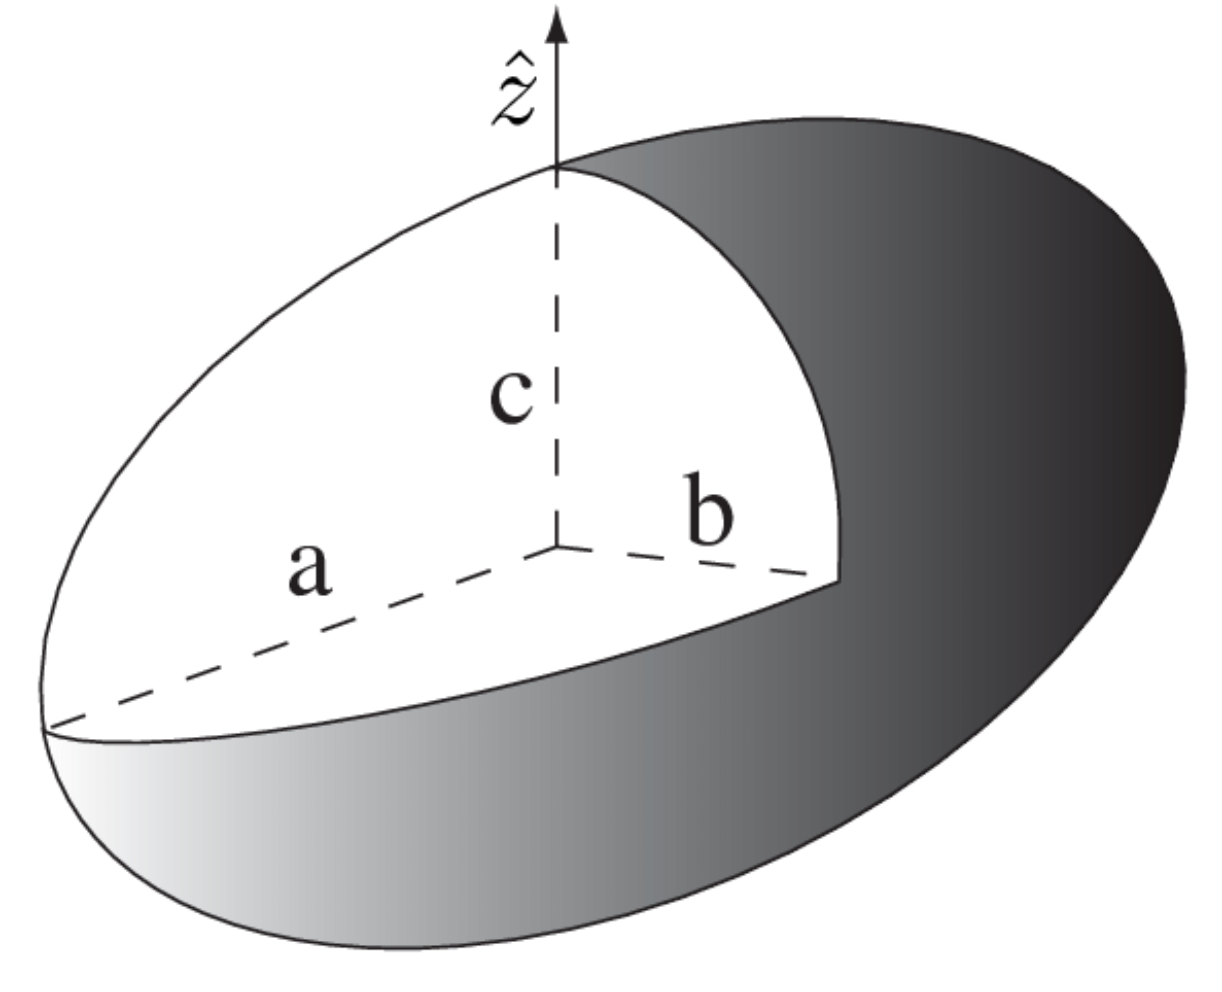
\includegraphics[width=0.35\linewidth]{graphics/tri-axial.png}
    \caption{Tri-axial ellipsoid model \textmd{of homogeneous mass distribution $\rho$, with $I_x<I_y<I_z$, respectively with axes a, b, and c.}}
    \label{fig:tri-axial-model}
\end{figure}

This model is illustrated in \autoref{fig:tri-axial-model} with $I_x<I_y<I_z$.
This model corresponds to the convention of body-fixed frames which have their
$Z$-axis aligned with the rotational axis of the body, however due to precession
and nutation, the true $Z$-axis of date representing the current rotation axis
will differ from the geometrical $\hat{Z}$-axis of the tri-axial ellipsoid. The
period of precession and nutation for short time scales however can be omitted
and for studies which does not involve long term analysis of the subsequent
effects, $Z\approx{\hat{Z}}$. There is a closely related model which is the next
step taken by astrodynamacists after a point mass approximation in missions
design, which is the use of an oblate spheroid. This is often used to account
for the mass concentration at the equator of Earth. This model is obtained from
the homogeneous tri-axial ellipsoid by simply setting $b=a$. The gravitational
potential, $U$, using this model with elliptical integrals, of a body in its
body-fixed reference frame $\{X^B\}$ is

\begin{equation}
    U(\mathbf{r})=\frac{3}{4}\mu \int_{\kappa_0}^{\infty}\bigg(1-\frac{{r_x}^2}{a^2+\kappa} - \frac{{r_y}^2}{b^2+\kappa} - \frac{{r_z}^2}{c^2+\kappa}\bigg)\cdot{}\frac{d\kappa}{\sqrt{((a^2+\kappa)(b^2+\kappa)(c^2+\kappa))}}
    \label{eq:triaxial_ellipsoid_potential_elliptic_integral}
\end{equation}

\begin{equation*}
    \begin{aligned}
        \textrm{where, }
        \kappa &= \textrm{parameter of the pencil for a confocal ellipse}\\
        \kappa_0 &= \textrm{largest root of the confocal ellipsoid}\\
        a, b, c &= \textrm{length of ellipsoid axes, respectively in the x, y and z directions of the body-fixed frame $\{X^B\}$.}
    \end{aligned}
\end{equation*}

\begin{equation}
    C(\kappa) = \frac{{r_x}^2}{a^2+\kappa} + \frac{{r_y}^2}{b^2+\kappa} + \frac{{r_z}^2}{c^2+\kappa} - 1.
\end{equation}

The expressions above are attributed to \cite{Ivory1809}, a detailed derivation
is given by Mac Millan \cite{MacMillan1958}, Danby \cite{Danby1992} and Moulton
\cite{moulton1970introduction}. The integrals seen in
\autoref{eq:triaxial_ellipsoid_potential_elliptic_integral} are elliptic
integrals. By use of Legendre's canonical elliptic integrals of first kind $F$
and second kind $E$, it is possible to find an expression for $U$ and it's
derivatives. Alternatively, as demonstrated by Willis et al. \cite{Willis2016},
a more modern approach using Carlson elliptic integrals. After introducing
$\kappa'=\kappa-\kappa_0$ in
\autoref{eq:triaxial_ellipsoid_potential_elliptic_int}, the gravitational
potential becomes,

\begin{equation}
    \begin{aligned}
        U(\mathbf{r}) &= \frac{3}{2}\mu{R_F}(a^2+\kappa_0, b^2 + \kappa_0, c^2 + \kappa_0)\\
        &- \frac{1}{2}\mu{{r_x}^2}R_D(b^2 + \kappa_0, c^2+\kappa_0, a^2+\kappa_0)\\
        &- \frac{1}{2}\mu{{r_y}^2}R_D(a^2 + \kappa_0, c^2+\kappa_0, b^2 + \kappa_0)\\
        &- \frac{1}{2}\mu{{r_z}^2}R_D(a^2 + \kappa_0, b^2 + \kappa_0, c^2 + \kappa_0),
    \end{aligned}
\end{equation}


where $R_F(x, y, z)$ and $R_{D}(x, y, z)$ are two of the Carlson symmetric forms, and their incomplete elliptic integrals are

\begin{equation}
    R_F(x, y, z) = \frac{1}{2}\int_0^\infty\frac{dt}{\sqrt{(t+x)(t+y)(t+z)}},
    \label{eq:r_f}
\end{equation}
\begin{equation}
    R_D(x, y, z) = \frac{3}{2}\int_0^\infty\frac{dt}{(t+x)\sqrt{(t+x)(t+y)(t+z)}}.
    \label{eq:r_d}
\end{equation}

The numerical evaluation of the above expressions (\autoref{eq:r_f} and
\autoref{eq:r_d}) are detailed by Johansson \cite{Johansson2019}. The
acceleration due to the gravitational potential then becomes:

% \begin{equation}
%     \begin{aligned}
%     a_{g_x} = \frac{\partial{V}}{\partial{x}} = \mu{r_x}{R_D(b^2 + \kappa_0, c^2 + \kappa_0, a^2 + \kappa_0)}\\
%     a_{g_y} = \frac{\partial{V}}{\partial{y}} = \mu{r_y}{R_D(a^2 + \kappa_0, c^2 + \kappa_0, b^2 + \kappa_0)}\\
%     a_{g_z} = \frac{\partial{V}}{\partial{y}} = \mu{r_z}{R_D(a^2 + \kappa_0, b^2 + \kappa_0, c^2 + \kappa_0)}\\
%     \end{aligned}
% \end{equation}
\begin{equation}
    \bm{a}_g
    =
    \begin{bmatrix}
        a_{g_x} \\
        a_{g_y} \\
        a_{g_z}
    \end{bmatrix}
    =
    \nabla_\mathbf{r}{U}
    =
    \begin{bmatrix}
        \frac{\partial{U}}{\partial{x}} \\
        \frac{\partial{U}}{\partial{y}} \\
        \frac{\partial{U}}{\partial{z}}
    \end{bmatrix}
    =
    \begin{bmatrix}
        \mu{r_x}{R_D(b^2 + \kappa_0, c^2 + \kappa_0, a^2 + \kappa_0)} \\
        \mu{r_y}{R_D(a^2 + \kappa_0, c^2 + \kappa_0, b^2 + \kappa_0)} \\
        \mu{r_z}{R_D(a^2 + \kappa_0, b^2 + \kappa_0, c^2 + \kappa_0)} \\
    \end{bmatrix}
\end{equation}


%%%%%%%%%%%%%%%%%%%%%%%%%%%%%%%%%%%%%%%%%%%%%%%%%%%%%%%%%%%%%%%%%%%%%%%%%%%%%%%%
\subsection{Expansion in spherical harmonics}
%%%%%%%%%%%%%%%%%%%%%%%%%%%%%%%%%%%%%%%%%%%%%%%%%%%%%%%%%%%%%%%%%%%%%%%%%%%%%%%%

The general approach for high fidelity gravitational potential modelling is the
use of spherical harmonic expansion. The gravitational potential, $U$, of a
body, in its body-fixed reference frame $\{X^B\}$ is described by the infinite
series

\begin{equation}
    U(r,\phi,\lambda) = \frac{GM}{r}\sum_{n=0}^\infty{}\sum_{m=0}^n{}\bigg[\bigg(\frac{R}{r}\bigg)^l\times{}\overline{P}_{nm}(\sin{\phi})(\overline{C}_{nm}\cos{m\lambda}+\overline{S}_{nm}\sin{m\lambda})\bigg],
    \label{eq:grav_sh}
\end{equation}
\begin{equation*}
    \begin{aligned}
        \textrm{where, }
        r, \phi, \lambda &= \textrm{spherical coordinates in $\{X^B\}$, respectively the radius coordinate, latitude and longitude,} \\
        G &= \textrm{universal gravitational constant,} \\
        M &= \textrm{mass of body,} \\
        n, m &= \textrm{respectively the degree and order of a particular spherical harmonic,} \\
        R &= \textrm{reference radius,} \\
        \overline{P}_{nm} &= \textrm{the normalized associated Legendre polynomials,} \\
        \overline{C}_{nm}, \overline{S}_{nm} &= \textrm{the normalized spherical harmonic coefficients,} \\
    \end{aligned}
\end{equation*}

This expansion is infinite in priciple and may be truncated in practice
depending on the degree of knowledge of the body surface or gravitational
potential field. The degree and order to which the spherical harmonics are
expanded are determined by the quantity and quality of empirical observations.
These observations constrain the the certainty associated to the harmonic
coefficients in the expansion. The general approach is to fit higher fidelity
expansions, until the residual error between observation and model converge
towards a random normal distribution. This convergence suggests that only
stochastic error sources remain, which cannot be modelled deterministically.
These error sources are usually due to the limitation of the hardware employed
in the collection of measurements.

% Recent models for the Earth, Venus and Mars shapes, complete to degree 1080, 720, and 720 respectively, have been recently
% determined (Balmino, 1993); a model of degree 12 exists for the Moon (Bills
% and Ferrari, 1977) and a model of degree 8 has been established for Phobos by
% Duxbury (1991).

%%%%%%%%%%%%%%%%%%%%%%%%%%%%%%%%%%%%%%%%%%%%%%%%%%%%%%%%%%%%%%%%%%%%%%%%%%%%%%%%
\subsection{Tri-axial ellipsoid: expansion in spherical harmonics}
%%%%%%%%%%%%%%%%%%%%%%%%%%%%%%%%%%%%%%%%%%%%%%%%%%%%%%%%%%%%%%%%%%%%%%%%%%%%%%%%

The expansion in spherical harmonics may be easily expanded to represent a
homogeneous distribution of mass as a tri-axial ellipsoid, providing a bridge to
the elliptic integral representation presented previously. This expansion is
demonstrated by Balmino \cite{Geodesy1994}. After introducing the mass
$M=\frac{4}{3}\pi{abc\rho}$, it is demonstrated that,

\begin{equation}
    \begin{aligned}
        C_{2l,2m}&=\frac{3}{R^{2l}}\frac{l!(2m)!}{2^{2l}(2l+3)(2l+1)!}(2-\delta_{0m})\frac{(2l-2m)!}{(2l + 2m)!}\\
        &\times \sum_{k=0}^{l-m}\frac{(-1)^k(4l-2k)!}{(2l-k)!(2l-2m-2k)!}\\
        &\times
        \sum_{s=0}^{m}\frac{(-1)^s}{(2s)!(2m-2s)!}\sum_{p=0}^k\frac{(2l-2m-2p)!}{(l-m-p)!(k-p)!}\\
        &\times
        \sum_{q=0}^{p}\frac{(2s+2p-2q)!(2m-2s+2q)!}{q!(p-1)!(s+p-q)!(m-s+q)!}\\
        &\times a^{2(m-s+q)}b^{2(s+p-q)}c^{2(l-m-p)},
    \end{aligned}
\end{equation}

where, for example, it is found that,
\begin{equation}
    \begin{aligned}
        C_{20}&=\frac{1}{5R^2}\bigg(c^2-\frac{a^2+b^2}{2}\bigg),\\\vspace{3mm}
        C_{22}&=\frac{1}{20R^2}(a^2-b^2),\\\vspace{3mm}
        C_{40}&=\frac{15}{7}(C_{20}^2+2C_{22}^2),\\\vspace{3mm}
        C_{42}&=\frac{5}{7}C_{20}C_{22},\\\vspace{3mm}
        C_{44}&=\frac{5}{28}C_{22}^2.\\\vspace{3mm}
    \end{aligned}
\end{equation}

It is further noted by Balmino \cite{Geodesy1994} that there is a uniform
convergence condition for \autoref{eq:grav_sh} in the case of the homogenous
tri-axial ellipsoid equivalent expansion, which is $a<c\sqrt{2}$.

% \begin{equation}
%     \begin{aligned}
%     \overline{P}_{nm}(u) &= (1-u^2)^{m/2}\frac{d^m}{du^m}P_n(u)\\
%     \overline{C}_{nm} &= \\
%     \overline{S}_{nm} &= \\
%     \overline{P}_n(u) &= \frac{1}{2^{n}n!}\frac{d^n}{du^n}(u^2-1)^n\\
%     \end{aligned}
% \end{equation}

% \subsection{Expansion in spheroidal harmonics}

% \begin{equation}
%     V(r, \theta, \lambda) = 
% \end{equation}


% \section{Measurement Uncertainty}

% \begin{equation}
%     s_i = s_i + s_i · N(0, \sigma_{SN})
% \end{equation}

    \section{Numerical Analysis}

\subsection{Initial value problems}

\subsection{Integration methods}

\subsection{Mesh refinement}
\subsubsection{Reducing element size: h-method}
\subsubsection{Increasing element order: p-method}
\subsubsection{Optimising element location: r-method}

\subsection{Interpolation methods}
    %%%%%%%%%%%%%%%%%%%%%%%%%%%%%%%%%%%%%%%%%%%%%%%%%%%%%%%%%%%%%%%%%%%%%%%%%%%%%%%%
\chapter{Trajectory Optimization}
%%%%%%%%%%%%%%%%%%%%%%%%%%%%%%%%%%%%%%%%%%%%%%%%%%%%%%%%%%%%%%%%%%%%%%%%%%%%%%%%
Trajectory optimisation is the process of designing a series of states across a
temporal dimension that maximizes (or minimizes) a measure of performance. This
technique is generally used to obtain the open-loop solution of an optimal
control problem within a finite horizon. Due to the common presence of
nonlinearities in the constraint and/or performance functions, trajectory
optimisation problems often employ the use of \textit{nonlinear programming}.

Mathematicaly the problem can be described by $N$ phases, with the independent
variable $t$, where phase $k$ lies within the region
$t_0^{(k)}\leq{t}\leq{t_f^{(k)}}$. The independent variable $t$ very often
describes \text{time} within mosr practical applications, where the phases are
sequential, that is $t_0^{(k+1)}=t_f^{(k)}$, however as stated by
\textit{Betts}, and demononstrated well by \autoref{sec:sundmann}, neither of
these assumptions are required. In phase $k$, the dynamic variables are
described as,
\begin{equation}
  \mathbf{z}=
  \begin{bmatrix}
  \mathbf{x}^{(k)}(t) \\
  \mathbf{u}^{(k)}(t)
  \end{bmatrix},
\end{equation}
where $\mathbf{x}_k$ and $\mathbf{u}_k$ describe the \textit{state variables}
and \textit{control variables} respectively at the $n$ knot points.
bash -ic \usr\bin\pdflatex -file-line-error -interaction=nonstopmode -synctex=1 -output-format=pdf \"-output-directory=/mnt/c/Users/ggarr/OneDrive/Documents/Literature Study/out\" /mnt/c/Users/ggarr/OneDrive/Documents/Literature Study/main.tex

%%%%%%%%%%%%%%%%%%%%%%%%%%%%%%%%%%%%%%%%%%%%%%%%%%%%%%%%%%%%%%%%%%%%%%%%%%%%%%%%
\section{Sims-Flanagan Method}
%%%%%%%%%%%%%%%%%%%%%%%%%%%%%%%%%%%%%%%%%%%%%%%%%%%%%%%%%%%%%%%%%%%%%%%%%%%%%%%%
A common method for low-thrust trajectory optimisation in numerical
astrodynamics, the Sims-Flanagan method \cite{Sims2000}, is the optimisation of
a low-thrust trajectory following transcription into a series of conic arcs
connected by $\Delta{V}$ impulses, as seen in Figure \autoref{fig:sf}.

\begin{figure}[H]
    \centering
    \label{fig:sf}
%    \includegraphics[width=0.4\textwidth]{graphics/1/sims-flanagan-izzo}
    \caption{
        Impulsive $\Delta{V}$ transcription of a low-thrust trajectory, after
        Sims and Flanagan \cite{Yam2010}.
    }
\end{figure}

This method is fast and robust, however due to its discretization of a
continuous low-thrust problem, it can fail to be a faithful representation of
reality. Yam et al. improve upon this method in two ways: 1) the $\Delta{V}$
impulses are replaced with continuous thrust where the low-thrust arcs are
numerically propagated; and 2) the time mesh, or series of knot points, are
optimised together with the trajectory.

%%%%%%%%%%%%%%%%%%%%%%%%%%%%%%%%%%%%%%%%%%%%%%%%%%%%%%%%%%%%%%%%%%%%%%%%%%%%%%%%
\section{Sundmann Transform\label{sec:sundmann}}
%%%%%%%%%%%%%%%%%%%%%%%%%%%%%%%%%%%%%%%%%%%%%%%%%%%%%%%%%%%%%%%%%%%%%%%%%%%%%%%%
Karl Sundman introduced a simple transformation for the time variable, to
regularize the otherwise singular three body problem. A new variable $s$ is
introduced through the relation $ds=dt/r$ which \textit{guarantees an
asymptotically slower flow} near the singularities ~\cite{Sundman1913}.

\begin{equation}
    \begin{aligned}
        r&=\sqrt{x_1 ^2 + x_2 ^ 2 + x_3 ^ 2}\\
        \dot{x}_1 &= x_{4}r\\
        \dot{x}_2 &= x_{5}r\\
        \dot{x}_3 &= x_{6}r\\
        \dot{x}_4 &= -x_{1}/r^2+u_1{r}\\
        \dot{x}_5 &= -x_{2}/r^2+u_2{r}\\
        \dot{x}_6 &= -x_{3}/r^2+u_3{r}\\
        \dot{t} &= r
    \end{aligned}
\end{equation}
Yam et al. demonstrates quite effectively that sampling in the $s$ domain is
useful for trajectory optimization. \cite{Yam2010} The difference between equal
sampling in the $s$ domain compared to that of time, is seen in Figure
\ref{fig:t-s}.

\begin{figure}[H]
    \centering
    \label{fig:t-s}
    \includegraphics[width=0.8\textwidth]{graphics/1/sampling-t-s}
    \caption{
        A trajectory sampled with the same number of a) time spaced segments b)
        s-spaced segments \cite{Yam2010}.
    }
\end{figure}

It is evident from Figure \ref{fig:t-s} that sampling the $s$ domain is superior
in generating a smooth trajectory, in the context of orbital trajectory
discretization. \textcolor{blue}{This presents an interesting aspect when one
considers replacing the temporal variable of time with the s-domain in the
context of an infinite-horizon reinforcement learning problem.}

%%%%%%%%%%%%%%%%%%%%%%%%%%%%%%%%%%%%%%%%%%%%%%%%%%%%%%%%%%%%%%%%%%%%%%%%%%%%%%%%
\section{Optimal Control}
%%%%%%%%%%%%%%%%%%%%%%%%%%%%%%%%%%%%%%%%%%%%%%%%%%%%%%%%%%%%%%%%%%%%%%%%%%%%%%%%

%%%%%%%%%%%%%%%%%%%%%%%%%%%%%%%%%%%%%%%%%%%%%%%%%%%%%%%%%%%%%%%%%%%%%%%%%%%%%%%%
\subsection{Potryagins maximum principal}
%%%%%%%%%%%%%%%%%%%%%%%%%%%%%%%%%%%%%%%%%%%%%%%%%%%%%%%%%%%%%%%%%%%%%%%%%%%%%%%%

%%%%%%%%%%%%%%%%%%%%%%%%%%%%%%%%%%%%%%%%%%%%%%%%%%%%%%%%%%%%%%%%%%%%%%%%%%%%%%%%
\subsection{Model predictive control (MPC)}
%%%%%%%%%%%%%%%%%%%%%%%%%%%%%%%%%%%%%%%%%%%%%%%%%%%%%%%%%%%%%%%%%%%%%%%%%%%%%%%%

%%%%%%%%%%%%%%%%%%%%%%%%%%%%%%%%%%%%%%%%%%%%%%%%%%%%%%%%%%%%%%%%%%%%%%%%%%%%%%%%
\subsection{Recent Research}
%%%%%%%%%%%%%%%%%%%%%%%%%%%%%%%%%%%%%%%%%%%%%%%%%%%%%%%%%%%%%%%%%%%%%%%%%%%%%%%%

%%%%%%%%%%%%%%%%%%%%%%%%%%%%%%%%%%%%%%%%%%%%%%%%%%%%%%%%%%%%%%%%%%%%%%%%%%%%%%%%
\subsubsection{Autoencoder of coordinates}
%%%%%%%%%%%%%%%%%%%%%%%%%%%%%%%%%%%%%%%%%%%%%%%%%%%%%%%%%%%%%%%%%%%%%%%%%%%%%%%%

\url{https://www.youtube.com/watch?v=KmQkDgu-Qp0}

    \section{Linearization}

Given the complexity of the models which depend on a variety of
parameters which are used in the description of the dynamic motion or
measurement process, it is customary to linearize the relations between
observables and the independent parameters in order to obtain expressions which
are more easily handled.

\subsection{Taxonomy of Partials}
\subsubsection{The State Transition Matrix}

Let the state vector $\mathbf{y(t)}$ of the dynamic system at an arbitrary epoch
$t$ be the concatenation of the position $\mathbf{r}(t)$ and velocity vector
$\mathbf{v}(t)$. A state vector at a specified epoch is given by
$\mathbf{y}(t_0)$. The state transition matrix $\bm{\Phi}(t,t_0)$ describes the
change of the state vector at a time $t$ due to a change in the initial state
vector at time $t_0$

\begin{equation}
    \bigg(\frac{\partial\mathbf{y}(t)}{\partial{\mathbf{y}(t_0)}}\bigg)_{6\times{6}}=\bm{\Phi}(t, t_0).
    \label{eq:linear_stm}
\end{equation}

\subsubsection{The Sensitivity Matrix}

For a given set of $n_p$ parameters which are dependent variables in
the calculation of acceleration acting on on the system of bodies $\mathbf{p}$,
their dependence is described by the sensitivity matrix, i.e. the partial
derivatives

\begin{equation}
    \bigg(\frac{\partial\mathbf{y}(t)}{\partial{\mathbf{p}}}\bigg)_{6\times{n_p}}=\bm{S}(t)
\end{equation}

with respect to the force model parameters. The parameters $p$ often include
coefficients which are empirical in nature, these include but are not limited to
the coefficients of lift, drag, and radiation pressure.

\subsubsection{Partials of measurements with respect to the state vector}
The linearized dependence of 

\subsection{Solar Radiation Pressure}

\subsubsection{Partial derivative with respect to state}

\begin{equation}
    \frac{\partial{\bm{a}_{s}}}{\partial{\mathbf{r}}} =
    -P_\Sun\frac{A}{m}\frac{AU^2}{r^5}
    \begin{bmatrix}
    3r_x^2-r^2 & 3r_xr_y    & 3r_xr_z \\
    3r_yr_x    & 3r_y^2-r^2 & 3r_yr_z \\
    3r_zr_x    & 3r_zr_y    & 3r_z^2-r^2 \\
    \end{bmatrix}
    \label{eq:partial_srp_state}
\end{equation}

\subsubsection{Partial derivative with respect to coefficient of radiation pressure}

\begin{equation}
    \frac{\partial\bm{a}_{s}}{\partial{C_r}}
    =
    \frac{1}{C_R}\bm{a}_s
    =
    -P_\Sun\frac{A}{m}\frac{\mathbf{r}}{r^3}AU^2
    \label{eq:partial_srp_cr}
\end{equation}

\subsection{Thrust}

\begin{equation}
    \frac{\bm{a}_T}{\partial{}}
\end{equation}

\subsection{Gravitational Potential: Point Mass}

\subsubsection{Partial derivative with respect to state}
\begin{equation}
    \frac{\partial{\bm{a}_{g}}}{\partial{\mathbf{r}}}  =
    \frac{\mu}{r^5}
    \begin{bmatrix}
    3r_x^2-r^2 & 3r_xr_y    & 3r_xr_z \\
    3r_yr_x    & 3r_y^2-r^2 & 3r_yr_z \\
    3r_zr_x    & 3r_zr_y    & 3r_z^2-r^2 \\
    \end{bmatrix}
    \label{eq:partial_point_mass_wrt_state}
\end{equation}

\subsubsection{Partial derivative with respect to gravitational parameter}
\begin{equation}
    \frac{\partial{\bm{a}_{g}}}{\partial{\mu}} =
    \frac{1}{\mu}\bm{a}_g =
    -\frac{\mathbf{r}}{r^3}
    \label{eq:partial_point_mass_wrt_G}
\end{equation}

%%%%%%%%%%%%%%%%%%%%%%%%%%%%
\subsection{Gravitational Potential: Tri-axial ellipsoid}
\subsubsection{Partial derivative with respect to state}
\begin{equation}
    \frac{\partial{\bm{a}_{g}}}{\partial{\mathbf{r}}} =
    \mu 
    \begin{bmatrix}
    
    \end{bmatrix}
    \label{eq:partial_triaxial_wrt_state}
\end{equation}

\subsubsection{Partial derivative with respect to characteristic parameters}
\begin{equation}
    \mathbf{p}_{g}=
    \begin{bmatrix}
    \rho & a & b & c \\
    \end{bmatrix}^T
\end{equation}

\begin{equation}
    j_1=
\end{equation}

\begin{equation}
    \frac{\partial{\bm{a}}_g}{\partial{\rho}} = 
    G\frac{4}{3}\pi
    \begin{bmatrix}
    {abc}{r_x}{R_D(b^2 + \kappa_0, c^2 + \kappa_0, a^2 + \kappa_0)}\\
    {abc}{r_y}{R_D(a^2 + \kappa_0, c^2 + \kappa_0, b^2 + \kappa_0)}\\
    {abc}{r_z}{R_D(a^2 + \kappa_0, b^2 + \kappa_0, c^2 + \kappa_0)}\\
    \end{bmatrix}
\end{equation}

\begin{equation}
    \frac{\partial{\bm{a}}_g}{\partial{\mathbf{p}_g}} = 
    G\frac{4}{3}\pi
    \begin{bmatrix}
    {abc}{r_x}{R_{D_x}} & \rho bc({r_x}{R_{D_x}} + a\frac{\partial{R_{D_x}}}{\partial{a}}) & \rho ac({r_x}{R_{D_x}} + b\frac{\partial{R_{D_x}}}{\partial{b}}) & \rho ab({r_x}{R_{D_x}} + c\frac{\partial{R_{D_x}}}{\partial{c}})\\
    {abc}{r_y}{R_{D_y}} & \rho bc({r_y}{R_{D_y}} + a\frac{\partial{R_{D_y}}}{\partial{a}}) & \rho ac({r_y}{R_{D_y}} + b\frac{\partial{R_{D_y}}}{\partial{b}}) & \rho ab({r_y}{R_{D_y}} + c\frac{\partial{R_{D_y}}}{\partial{c}})\\
    {abc}{r_z}{R_{D_z}} & \rho bc({r_z}{R_{D_z}} + a\frac{\partial{R_{D_z}}}{\partial{a}}) & \rho ac({r_z}{R_{D_z}} + b\frac{\partial{R_{D_z}}}{\partial{b}}) & \rho ab({r_z}{R_{D_z}} + c\frac{\partial{R_{D_z}}}{\partial{c}})\\
    \end{bmatrix}
\end{equation}

\subsection{Gravitational Potential: Expansion in spherical harmonics}

    
\newpage{}
\section{Observation Models}

\subsection{Landmark Tracking}
\textcolor{red}{Marie's Thesis + Michael. Model is similar to VLBI model.}

\textcolor{red}{2.1.1 In D.Dirkx for better notation.}

\textcolor{red}{Moyer, formulation for observed and computed quantities in DSN types.}
\subsection{Range Measurements/ Pseudorange}


\subsection{Doppler Measurements}

\subsubsection{Two-way Range Rate}
\begin{equation}
    \overline{\dot{\rho}}(t) = \frac{c}{2}\frac{(\tau_{2u}+\tau_{2d})-(\tau_{1u}+\tau_{2d})}{t_c} = \frac{1}{2}\frac{(\rho_{2u}+\rho_{2d})-(\rho_{1u} + \rho_{1d})}{t_c},
\end{equation}

\subsubsection{Range}

\subsubsection{One-Way Range Rate}
\begin{equation}
    \overline{\dot{\rho}} = c\frac{(\tau_2-\tau_1)}{t_c}=\frac{(\rho_2-\rho_1)}{t_c} 
\end{equation}

\subsubsection{Rational Doppler Bias}
\textcolor{red}{No real need to discuss, cut out in post processing.}
\begin{equation}
    \delta\overline{\dot{\rho}} = \frac{1}{t_c}\int_{t-t_c}^{t}d\cdot{\omega\sin{\alpha}\sin{\omega{t}}\;dt}
\end{equation}

\begin{equation}
    \Delta{\overline{\dot{\rho}}} = \frac{\lambda\omega}{2\pi}\frac{s_R+s_T/T_{1,2}}{2}
\end{equation}


\newpage{}

\section{Parameter Estimation}

\begin{itemize}
    \item Orbit of asteroid
    \item Orbit of spacecraft
    \item Rotation of asteroid (rate + principle axes)
    \item Gravitational potential of asteroid
\end{itemize}

\subsection{Orbit Determination}

\subsubsection{Weighted Least-Squares Estimation}

\begin{equation}
    H=\frac{\partial{\mathbf{h}}}{\partial{\mathbf{q}}}
\end{equation}

\begin{equation}
    \Delta{\mathbf{q}}=K(H^{T}W\Delta{\mathbf{h}})
\end{equation}

\begin{equation}
    K=(H^{T}WH)^{-1}
\end{equation}

\subsubsection{Linearization \& Normal Equations}

\subsubsection{Filtering}


 \noindent{}A CEKF consists of 3 main steps, namely: \textit{Initialisation (0)}, \textit{Prediction (1)} and \textit{Correction (2)}, where steps 1 \& 2 are iterated through $K-1$ times, where $K$ ($K\in\mathbb{Z}^+$) quantifies the number of Epochs.
 
 \begin{itemize}
     \item \textbf{Step (0) Initialisation}: The \textit{a posteriori} estimate of the initial state ($\hat{x}_0^+$) is determined according to the expectation of the true value $x_0$. The initial state error co-variance matrix is calculated according to the expectation of the co-variance between $\hat{x}_0^+$ and $x_0$. Within the context of satellite tracking, a predefined $\hat{x}_0^+$ will be used throughout the CEKF analysis to analyse the performance as a result of the selection of hyper-parameters: $\bm{Q}_{k-1}$ and $\bm{R}_k$.
     \item \textbf{Step (1) Prediction}: Project the state and its co-variance matrix at $k-1$ one step forward in order to obtain the \textit{a priori} estimates at $k$ according to the system dynamics. $\bm{Q}_{k-1}$ is implemented, then this contributes to the \textit{a priori} estimate of $P_k^{}$.
    \item \textbf{Step (2) Correction}: The measurements at $k$ are then compared with the predicted state according to system dynamics (\textit{a priori} estimate) providing the \textit{measurement innovation} ($\Delta{\rho}_k$). \textit{innovation co-variance} ($S_k$) and $H_k$ are then calculated and used to obtain the \textit{Kalman gain} ($\overline{K}_k$). Finally the \textit{a posteriori} estimate of the state ($\hat{x}_k^+$) and co-variance ($P_k^+$) are determined. $k$ is incremented by a step forward and the process from step 1 is repeated for all Epochs.
 \end{itemize}

\begin{figure}[htp]
    \centering
    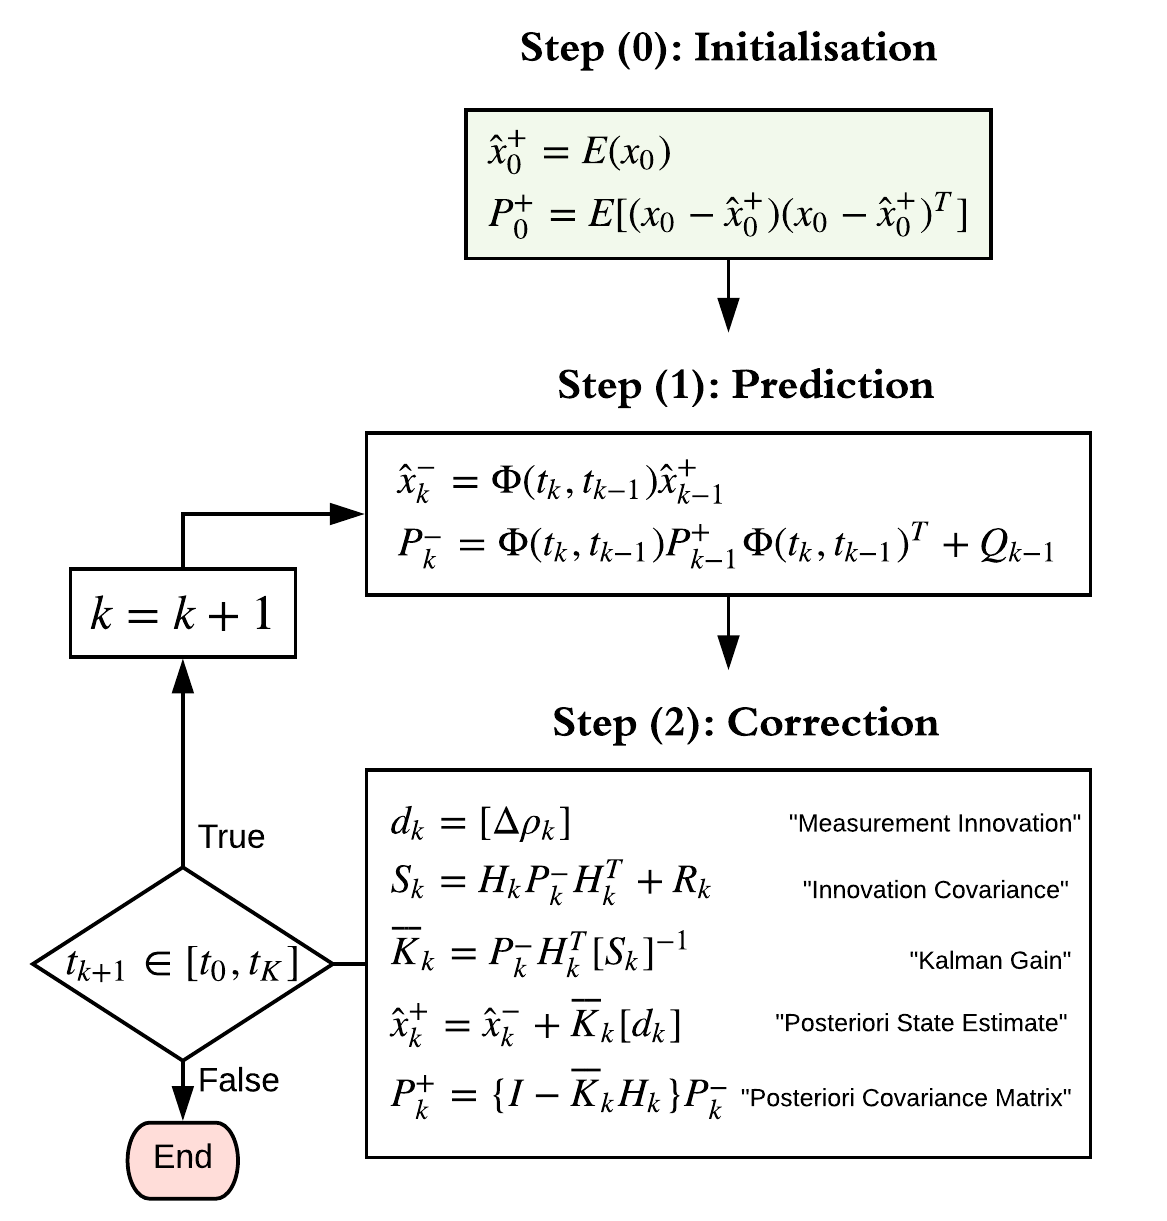
\includegraphics[width=0.55\linewidth]{graphics/CEKF.png}
    \caption{CEKF flow diagram for process of tracking and data prediction including all equations \cite{3}.}
    \label{fig:CEKF}
\end{figure}


\begin{figure}[htp]
    \centering
    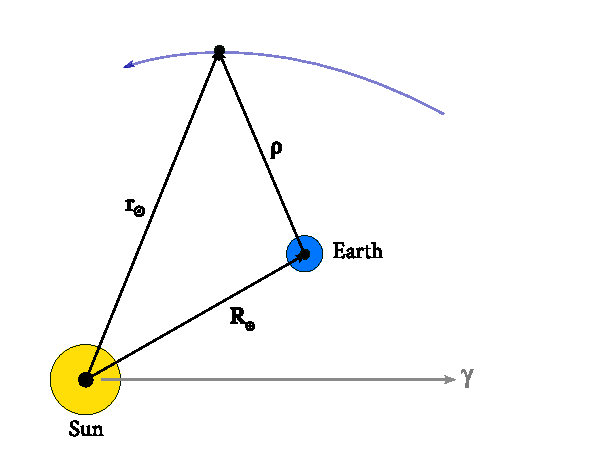
\includegraphics[width=0.5\linewidth]{graphics/pod-1.pdf}
    \caption{Orbit determination of asteroid using range observations from Earth ($\rho$).}
    \label{fig:my_label}
\end{figure}

\begin{equation}
    \rho = ||\mathbf{r}_\Sun - \mathbf{R}_\Earth||
\end{equation}


\begin{equation}
    \rho = ||\mathbf{r}_\Sun - \mathbf{R}_\Earth||
\end{equation}

\begin{itemize}
    \item \textbf{Orbit Determination}
    \item 
\end{itemize}

\subsection{Rotational State}

\subsection{Gravitational Potential}

\subsection{Shape}

\begin{itemize}
    \item \textbf{Rotation Model}: 
\end{itemize}
    %%%%%%%%%%%%%%%%%%%%%%%%%%%%%%%%%%%%%%%%%%%%%%%%%%%%%%%%%%%%%%%%%%%%%%%%%%%%%%%%
\chapter{Machine Learning\label{chap:ML}}
%%%%%%%%%%%%%%%%%%%%%%%%%%%%%%%%%%%%%%%%%%%%%%%%%%%%%%%%%%%%%%%%%%%%%%%%%%%%%%%%

% 2) A feedforward neural network, as formally defined in the article concerning feedforward neural networks, whose parameters are collectively denoted θ\thetaθ. In backpropagation, the parameters of primary interest are wijkw_{ij}^kwijk​, the weight between node jjj in layer lkl_klk​ and node iii in layer lk−1l_{k-1}lk−1​, and bikb_i^kbik​, the bias for node iii in layer lkl_klk​. There are no connections between nodes in the same layer and layers are fully connected.
% 3) An error function, E(X,θ)E(X, \theta)E(X,θ), which defines the error between the desired output yi⃗\vec{y_i}yi
%  and the calculated output yi⃗^\hat{\vec{y_i}}yi​​^​ of the neural network on input xi⃗\vec{x_i}xi​​ for a set of input-output pairs (xi⃗,yi⃗)∈X\big(\vec{x_i}, \vec{y_i}\big) \in X(xi​​,yi​​)∈X and a particular value of the parameters θ\thetaθ.

\Gls{ML}, often described as a proper subset of \gls{AI}
\cite{Goodfellow-et-al-2016}, and is the field in computer science which deals
with the improvement of algorithms through experience and the use of data
\cite{Mitchell97}. Our daily lives exhibit wide applications of intelligent
software to automate routine labour, understand speech or images, assist in
diagnoses in medicine and support basic scientific research. This field as a
whole is relatively young, having been coined in 1959 by Arthur Samuel
\cite{5392560}, however little progress in reaching human-comparable learning
was achieved until the advent of deep learning, termed by Rina Dechter in 1986
\cite{Rina1986}. Even then, human-like recognition of real-world images was not
achieved until ImageNet was created in 2009 \cite{5206848}, which is often
considered as the catalyst for the AI boom of the 21st century
\cite{hardy_2016}.

\begin{figure}[htp!]
    \centering
    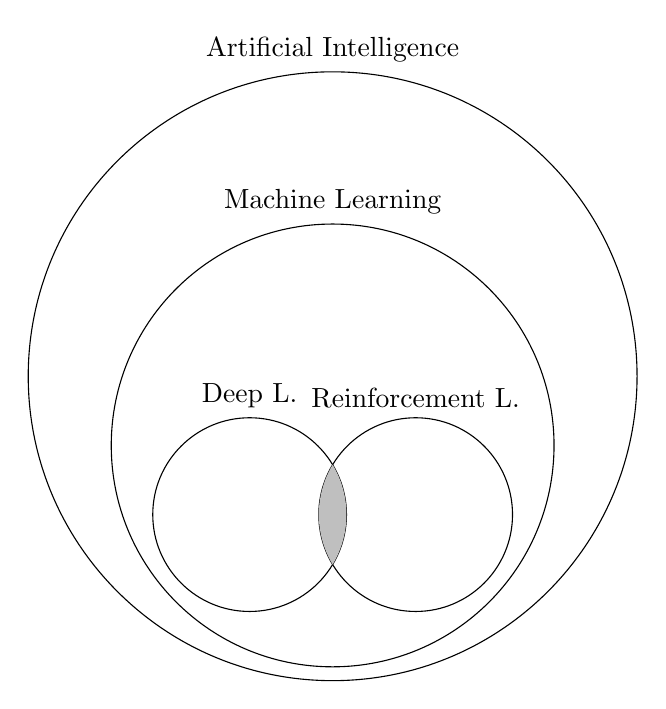
\begin{tikzpicture}

    % Circle with label
    \node[draw,
        circle,
        minimum size =22em,
        label=Artificial Intelligence] (ai_circ) at (0,0){};

    % Circle with label
    \node[draw,
        circle,
        minimum size =16em,
        label=Machine Learning] (ml_circ) at (0,-2.5em){};

    % Circle with label
    \node[draw,
        circle,
        minimum size =7em,
        label=Deep L.] (dl_circ) at (-3em,-5em){};

    \node[draw,
        circle,
        minimum size =7em,
        label=Reinforcement L.] (rl_circ) at (3em,-5em){};


    % Intersection
    \begin{scope}
        \clip (-3em,-5em) circle(3.5em);
        \clip (3em,-5em) circle(3.5em);
        \fill[gray!50](3em,-5em) circle(3.5em);
    \end{scope}

\end{tikzpicture}
    \captionsetup{format=hang} % hanging captions
    \caption{
        The relationship between the fields of Artificial Intelligence,
        Machine Learning, Deep Learning and Reinforcement Learning with some
        arbitrary example provided per field.
    }
    \label{fig:al-ml-dl}
\end{figure}


\newpage


\section{Machine Learning Basics}
%%%%%%%%%%%%%%%%%%%%%%%%%%%%%%%%%%%%%%%%%%%%%%%%%%%%%%%%%%%%%%%%%%%%%%%%%%%%%%%%
This section aims at a providing a non-exhaustive coverage of the basics of
machine learning can can be applied to all machine learning algorithms. This
section starts by defining what is meant when it is said that an algorithm
``learns". The types of datasets that may be encountered in the application of
these learning algorithms are then briefly covered to provide insight into the
potential applications which are not covered in this review. The distinction is
then made between the goal of fitting training data and the goal of finding
patterns that generalize to new data. This section then covers a very common
concept in machine learning: \textit{hyperparameters}, which are
\textit{settings} of a learning algorithm which must be determined outside the
learning algorithm itself.

\subsection{Learning algorithms}
%%%%%%%%%%%%%%%%%%%%%%%%%%%%%%%%%%%%%%%%%%%%%%%%%%%%%%%%%%%%%%%%%%%%%%%%%%%%%%%%
Generally speaking, a machine learning algorithm is a procedure for learning
from data.However correct this definition is, it provides little insight into
the relevant concepts in the field. A more succint definition is provided by
Mitchell \cite{Mitchell97LearningAlgorithm}:
\begin{quotation}
    \textit{A computer program is said to learn from experience $E$ with respect
    to some class of tasks $T$ and a performance measure $P$, if its performance
    at tasks in $T$, as measured by $P$, improves with experience $E$.}
\end{quotation}
This definition introduces the general entities which are present during all
machine learning tasks. The entities will not be formally defined in the
following sections as it is far outside the scope of this literature, and is
philosophical in nature. This section will instead cover examples of each which
will provide practical insight on which the reader can build their knowledge.

\subsubsection{The Task, $T$}
%%%%%%%%%%%%%%%%%%%%%%%%%%%%%%%%%%%%%%%%%%%%%%%%%%%%%%%%%%%%%%%%%%%%%%%%%%%%%%%%
There exists a plethora of tasks which humanity has applied learning algorithms
to during the timeline of the field. It is common for \gls{ML} practitioners to
originate from domains outside that of computer science, in order to access the
feasibility of existing algorithms in their domain. There is however a question
that often presents itself to specialists in their respective fields when they
consider applying \gls{ML} to the existing problems in their field. Why should a
specialist opt for solving problems with \gls{ML} that have been solved using
tried and true techniques in their domain of expertise? Goodfellow et al.
\cite{Goodfellow-et-al-2016} provide an insightful response to this:

\begin{quotation}
    \textit{Machine learning enables us to tackle tasks that are too difficult
    to solve with fixed programs written and designed by human beings. From a
    scientific and philosophical point of view, machine learning is interesting
    because developing our understanding of it entails developing our
    understanding of the principles that underlie intelligence. }
\end{quotation}
An example of a field which has undergone dramatic changes in a short period of
time, with the advent of \gls{DL} and modern hardware, is \gls{CV}. Mahony et.
al. discuss this in their paper with a focus on comparing \gls{DL} and \gls{CV}
\cite{Mahony-et-al-2020}. Their paper concludes that many \gls{CV} techniques
invented in the 20 years preceding the paper have become irrelevant as a result
of \gls{DL}. However, they emphasise on the importance of the knowledge
established in those 20 years, arguing that \textit{``knowledge is never
obsolete"}, as it provides specialists with more tools and intuition when
addressing problems. Some typical applications of \gls{CV} are detailed and
although these may be outperformed by \gls{DL}, relying on \gls{DL} in some
cases is overkill. They also point out some hybrid approaches between \gls{DL}
and \gls{CV} which synergize, saying that \gls{CV} provides improved performance
in \gls{DL} by reducing training time. This emphasises that specialists should
not expect an end-all solution from \gls{ML} in addressing their domain-specific
problems, but rather as mentioned by Goodfellow et al., strive for a better
understanding of the principles that underlie intelligence, and by extension,
those that underlie the practitioners domain-specific problems.

\begin{itemize}
    \item \textbf{Classification}: In this task, the learning algorithm is
    expected to produce a function $f: \mathbb{R^n}\rightarrow
    \{1,...,k\}$. When $y=f(\mathbf{x})$, the model assigns a provided
    input, $\mathbf{x}$ to a category identified by numeric code $y$. An
    example of this would be the mapping of a grayscale image,
    $\mathbf{x}\in\mathbb{R}^2$ to a value corresponding to a numerical
    encoding $f:\mathbb{R}^n\rightarrow\{\textrm{Cat},\;\textrm{Dog}\}$.
    \item \textbf{Classification with missing inputs}: Classification becomes
    more challenging when the input measurements to the model are not
    guaranteed to always be the same. In this situation the algorithm must
    learn the set of all function mappings arising from the possible
    combinations of input vectors that arise from missing subsets of
    inputs in $\mathbf{x}$. An example of this would be the classification
    of a diagnosis in medicine, as depending on the invasiveness of
    certain procedures, different subsets of measurements are available.
    \item \textbf{Regression}: In this task, the learning algorithm is expected
    to predict a continuous numerical value for a given input. This is
    done by learning a function $f: \mathbb{R}^n\rightarrow\mathbb{R}$.
    the formulation is similar to that of classification, except for the
    output format. An example of this would be learning of a function to
    predict the expected returns for a given investment given the state of
    the market, as is common is algorithmic trading.
    \item \textbf{Transcription}: This type of task involves the learning
    algorithm observing a relatively unstructured input and transcribing
    it into some discrete textual form. An example of this is the
    transcription of an audio waveform containing speech into text.
    \item \textbf{Machine translation}: In machine translation, the already
    structured input is mapped into a different language. This is common
    in the field of \gls{NLP}, where languages are translated between, for
    example English and French. This however is not limited to natural
    languages but can also be applied to programming languages for
    example.
    \item \textbf{Structured output}: This task entails those where the output
    is a vector or a data structure which details important relationships
    between the contained elements. This task subsumes the prior two of
    transcription and machine translation. An example of this would be the
    parsing of grammatical structure of a natural language sentence,
    addressed in \gls{NLP} and demonstrated by Collobert
    \cite{pmlr-v15-collobert11a}.
    \item \textbf{Anomaly detection}: In this task, a learning algorithm learns
    to sift through a set of events and classify events that are anomalous
    in nature. These algorithms have been applied to credit card companies
    in detection of fraud \cite{DBLP:journals/corr/abs-2108-10005}, and in
    safety in the aviation industry \cite{Janakiraman2016, Basora2019}.
    \item \textbf{Synthesis and sampling}: In this task, learning algorithms
    generate \textbf{new} examples which appear to be drawn from the same
    underlying distribution as, but are not present in the training data.
    A recent example around which a lot of research is being done is the
    \gls{GPT-3} which is able to produce human-like text, given prompts as
    input \cite{DBLP:journals/corr/abs-2005-14165}.
    \item \textbf{Imputation of missing values}: In this task, the learning
    algorithm is given some input $x\in\mathbb{R}$ with some elements
    $x_i$ missing. The algorithm must then make predictions for the
    missing values. Emmanuel et. al. discuss the latest methods in
    \gls{ML} that address this task~\cite{Emmanuel2021}.
    \item \textbf{Denoising}: In this learning task, the machine learning
    algorithm learns to generate a clean example $\mathbf{x}\in\mathbb{R}^n$
    from a corrupted sample $\tilde{\mathbf{x}}\in\mathbb{R}^n$. Generally
    speaking the learner is predicting the probability distribution
    $p(\mathbf{x}|\tilde{\mathbf{x}})$.
    \item \textbf{Density estimation} or \textbf{probability mass function estimation}
    involves the task task of learning a function $p_\text{model}:\mathbb{R}^n\rightarrow{}\mathbb{R}$,
    where $p_\text{model}(\mathbf{x})$ is interpreted as a probability distribution function
    from which $\mathbf{x}$ was drawn. Effectively the algorithm learns the
    structure of the data that it has been provided with. Most of the
    aforementioned tasks involve learning this distribution function, at least
    implicitly. For example for the missing value imputation task, if $x_i$ is
    missing, and all other values $x_{-i}$ are given, then the algorithm learns
    the distribution $p(x_i|\mathbf{x}_{-i})$ which involves $p(\mathbf{x})$
    implicitly.
\end{itemize}
%An ongoing trend in society is the augmentation of responsibility in intelligent
%algorithms through autonomy, evident by the advent of semi-autonomous cars,
%autonomous cyber-security \cite{Taeihagh2019}, autonomous industrial site
%inspection\footnote{\url{https://newsroom.ibm.com/Boston-Dynamics-and-IBM-Join-Forces-to-Bring-Mobile-Edge-Analytics-to-Industrial-Operations}},
%and autonomous supply-chain
%management\footnote{\url{https://www.forbes.com/sites/stevebanker/2021/04/01/amazon-supply-chain-innovation-continues/}},
%to name a few.

%This section reviews the current ongoing research in the field of machine
%learning as a whole. First the main categories:

\subsubsection{The Performance, $P$\label{sec:ML-performance}}
%%%%%%%%%%%%%%%%%%%%%%%%%%%%%%%%%%%%%%%%%%%%%%%%%%%%%%%%%%%%%%%%%%%%%%%%%%%%%%%%
In order to access the performance of our learning algorithm in task $T$,
we must have some quantitative measure of performance $P$ with which we steer
the algorithm towards the desired behaviour. $T$ and $P$ in this way are
coupled, and must $P$ must be chosen according to $T$. In this way it can be
unclear to the \gls{ML} practitioner what $P$ should be chosen.

Firstly, it is worth considering the true goal of the learning algorithm. We
wish for it to train according to some dataset such that it can generalize to
inputs that it has never seen before. After all, there is little worth in a
classification algorithm recognizing cats and dogs with 90\% accuracy on its
training dataset, if it performs with 20\% accuracy on an unseen \textbf{test}
dataset. This previously mentioned scenario is known as \textit{overfitting} and
is discussed in its own section later in the chapter. For this reason, the first
requirement on managing our dataset is presented, there must be some
\textbf{train-test split}. This is further complicated by the
\textbf{validation} dataset which is discussed later in the chapter.

Given that the input-output pair is $\{\mathbf{x}_i, \mathbf{y}_i\}$,
$\mathbf{y}_i$ is commonly referred to as the \textit{ground truth}, and
$\hat{\mathbf{f}}(\mathbf{x}_i)=\hat{\mathbf{y}}_i$ are referred to as the
\textit{predictor} and \textit{predicted output} respectively. The performance
in the form of a loss function $L$ is then some function of $\mathbf{y}_i$ and
$\hat{\mathbf{y}}_i$, therefore $L(\hat{\mathbf{y}}_i, \mathbf{y}_i)$.

\gls{ML} often borrows from \textit{approximation theory} vector norm notation
($\ell(\cdot)_p=||\cdot||_p$) to simplify notation in performance metrics. See
\autoref{appendix:vector_norms} for the expressions of vector norms.

\textbf{Regression loss functions}
\begin{itemize}
    \item \textbf{\Gls{MSE}} is the average of the squared differences between
    predictions and the ground truth. It is only concerned with the average
    magnitude of errors irrespective of their direction. Due to the squaring,
    predictions which have greater errors are more heavily penalized. A
    beneficial mathematical property of \gls{MSE} is that gradients can be
    easily calculated.
    \begin{equation}
        L_\text{MSE} = \frac{1}{N}\sum_{i=1}^{N}||\hat{\mathbf{y}}_i-\mathbf{y}_i||^2_2
    \end{equation}
    \item \textbf{L2 error} is the average of the differences between
    predictions and the ground truth. It is the same as \gls{MSE} but without
    the squaring. Like \gls{MSE}, the gradient can be easily calculated.
    \begin{equation}
        L_\text{L2E} = \frac{1}{N}\sum_{i=1}^{N}||\hat{\mathbf{y}}_i-\mathbf{y}_i||_2
    \end{equation}
    \item \textbf{\Gls{MAE}} or \textbf{L1 loss} is the average of the sum of
    absolute differences between predictions and the ground truth. This measure
    is similar to \gls{MSE} in that it considers the magnitude of the errors and
    ignores their direction. However, \gls{MAE} is more difficult to compute
    gradients for, requiring linear programming. \gls{MAE} is also more
    resilient to large error values as a result of outliers, as it does not make
    use of a square.
    \begin{equation}
        L_\text{MAE} = \frac{1}{N}\sum_{i=1}^{N}||\hat{\mathbf{y}}_i-\mathbf{y}_i||_1
    \end{equation}
    \item \textbf{\Gls{MBE}}
    \begin{equation}
        L_\text{MBE} = \frac{1}{N}\sum_{i=1}^{N}(\hat{\mathbf{y}}_i-\mathbf{y}_i)
    \end{equation}
    \item \textbf{\Gls{MSLE}}
    \begin{equation}
        \begin{aligned}
            L_\text{MSLE} &= \frac{1}{N}\sum_{i=1}^{N}(\log{(y_i+1)} - \log{(\hat{\mathbf{y}}_i+1)})^2 \\
            &= \frac{1}{N}\sum_{i=1}^{N}2\log(\frac{y_i+1}{\hat{\mathbf{y}}_i+1})
        \end{aligned}
    \end{equation}
    \item \textbf{Cosine Proximity}
    \begin{equation}
        L_\text{cos} = -\frac{\mathbf{y}_i\cdot{}\hat{\mathbf{y}}_i}{||\mathbf{y}_i||_2\cdot{}||\hat{\mathbf{y}}_i||_2}
    \end{equation}
\end{itemize}


\textbf{Binary classification loss functions}
\begin{itemize}
    \item Binary cross-entropy
    \begin{equation}
        L=-\sum_{i=1}^N\bigg(y_i\log(\hat{\mathbf{y}}_i)+(1-y_i)\log(1-\hat{\mathbf{y}}_i)\bigg)\label{eq:equation}
    \end{equation}
    \item Hinge loss
    \begin{equation}

    \end{equation}
    \item Squared hinge loss
\end{itemize}

\textbf{Multi-class classification loss functions}
\begin{itemize}
    \item Multi-class cross-entropy
    \begin{equation}
        L_{CE}=-\sum_{i=1}^N\sum_{j=1}^{M}y_{ij}\log(\hat{f}_j(\mathbf{x}_i))
    \end{equation}
    \item Hinge loss
    \item Squared hinge loss
\end{itemize}


\begin{itemize}
\end{itemize}
%With the
%In the case of classification, most metrics are derived from the confusion
%matric

\subsubsection{The Experience, $E$\label{sec:ML-experience}}
%%%%%%%%%%%%%%%%%%%%%%%%%%%%%%%%%%%%%%%%%%%%%%%%%%%%%%%%%%%%%%%%%%%%%%%%%%%%%%%%
Tasks provided to machine learning algorithms have different formulations based
on the experience made available. Learning algorithms can be broadly categorized
by the kind of experience that the algorithm has access to during learning, from
which it is generally expected to learn some pattern of interest.

\begin{itemize}
    \item \textbf{Supervised learning} algorithms experience a dataset
    containing features (input) and labels (expected output), and are expected
    to learn a function mapping between the two. These algorithms can be further
    divided into two categories. \textbf{Classification algorithms} learn a
    mapping from an input to a discrete class label output. \textbf{Regression
    algorithms} learn a mapping from an input to a continuous value output.

%    example input-output pairs, otherwise referred to as the labelled training
%    data consisting of a set of training examples. The trained \textit{model} is
%    then provided an unseen $x$ for which it must estimate $y$ based on its
%    experience. Supervised models are further grouped into two subcategories,
%    classification and regression. \textbf{Classification} is the task of
%    mapping $x$ to a discrete output variable $y$ which determines the predicted
%    class based on the $x$. A simple example of this would be a $y$ in
%    $\mathbb{R}^2$ which determines whether the input image was a \textit{cat}
%    or a \textit{dog}. \textbf{Regression} is task of mapping $x$ onto a
%    continuous output variable $y$ which determines the value of some variable
%    of interest. An example of this would be the task of learning an
%    approximator to the function: $f(x)=x^2$.
    % Dimensionality reduction \cite{vogelstein2021supervised}

    \item \textbf{Unsupervised learning} algorithms experience a dataset
    containing only features and learn some useful properties of the structure
    of the dataset. This form of learning often addresses recognition problems
    in \textit{association} \& \textit{clustering} \cite{barlow1999ul}.

    \item \textbf{Semi-supervised} is a middle ground between supervised
    learning (in which all training data is labelled) and unsupervised learning
    (in which no label data is provided)~\cite{books/mit/06/CSZ2006}. Some
    example applications of this paradigm are dimensionality reduction
    ~\cite{Zhang2007}, clustering \cite{Bair2013}, and anomaly detection
    \cite{DBLP:journals/corr/abs-1805-06725}.

    \item \textbf{Reinforcement learning} are learning algorithms which rely
    exclusively on a series of reinforcements from its environment. These
    reinforcements can be positive (rewards) or negative (punishments). This
    category is discussed further in \autoref{ssec:RL}.
\end{itemize}

\subsection{Capacity, Overfitting and Underfitting}
%%%%%%%%%%%%%%%%%%%%%%%%%%%%%%%%%%%%%%%%%%%%%%%%%%%%%%%%%%%%%%%%%%%%%%%%%%%%%%%%
The primary objective in \gls{ML} is to find a model which performs well on
previously \textit{unseen data}, which has not been used during the training or
fitting of a model. This ability of the learning algorithm is referred to as the
\textit{generalisation}.

Typically the learning algorithm is trained according to a set of
\textit{training data} with which we aim at reducing the learners
\textbf{training error}. Due to this data having been directly used to optimise
the moding during training, we cannot expect this error to be representative of
the \textbf{generalisation error}. In order to derive an estimate of the
generalisation error, we separate part of the initial data set into training and
\textbf{test data}, from which the \textbf{test error} is derived. Given some
assumptions about the \textbf{data-generating process}, it can be said that the
test error is equal to the expected generalisation error of the mode.

An important concept in \gls{ML} is the \textit{capacity} of the model. This is
defined informally as \textit{``a model’s [...] ability to fit a wide
variety of functions"}~\cite[p.~111-112]{Goodfellow-et-al-2016}.

\begin{figure}[htp]
    \centering
    % MIT License
%
% Copyright (c) 2021 Geoffrey H. Garrett
%
% Permission is hereby granted, free of charge, to any person obtaining a copy
% of this software and associated documentation files (the "Software"), to deal
% in the Software without restriction, including without limitation the rights
% to use, copy, modify, merge, publish, distribute, sublicense, and/or sell
% copies of the Software, and to permit persons to whom the Software is
% furnished to do so, subject to the following conditions:
%
% The above copyright notice and this permission notice shall be included in all
% copies or substantial portions of the Software.
%
% THE SOFTWARE IS PROVIDED "AS IS", WITHOUT WARRANTY OF ANY KIND, EXPRESS OR
% IMPLIED, INCLUDING BUT NOT LIMITED TO THE WARRANTIES OF MERCHANTABILITY,
% FITNESS FOR A PARTICULAR PURPOSE AND NONINFRINGEMENT. IN NO EVENT SHALL THE
% AUTHORS OR COPYRIGHT HOLDERS BE LIABLE FOR ANY CLAIM, DAMAGES OR OTHER
% LIABILITY, WHETHER IN AN ACTION OF CONTRACT, TORT OR OTHERWISE, ARISING FROM,
% OUT OF OR IN CONNECTION WITH THE SOFTWARE OR THE USE OR OTHER DEALINGS IN THE
% SOFTWARE.

%%%%%%%%%%%%%%%%%%%%%%%%%%%%%%%%%%%%%%%%%%%%%%%%%%%%%%%%%%%%%%%%%%%%%%%%%%%%%%%
% ACKNOWLEDGEMENTS
%%%%%%%%%%%%%%%%%%%%%%%%%%%%%%%%%%%%%%%%%%%%%%%%%%%%%%%%%%%%%%%%%%%%%%%%%%%%%%%
% Design and implementation of this diagram was inspired and adapted from:
% https://tex.stackexchange.com/questions/573127/tikz-plots-are-not-centered

%%%%%%%%%%%%%%%%%%%%%%%%%%%%%%%%%%%%%%%%%%%%%%%%%%%%%%%%%%%%%%%%%%%%%%%%%%%%%%%
% DEPENDENCIES
%%%%%%%%%%%%%%%%%%%%%%%%%%%%%%%%%%%%%%%%%%%%%%%%%%%%%%%%%%%%%%%%%%%%%%%%%%%%%%%
%\usepackage{tikz}
% \usetikzlibrary{positioning, decorations.text, calc}

%%%%%%%%%%%%%%%%%%%%%%%%%%%%%%%%%%%%%%%%%%%%%%%%%%%%%%%%%%%%%%%%%%%%%%%%%%%%%%%
% USER STYLING
%%%%%%%%%%%%%%%%%%%%%%%%%%%%%%%%%%%%%%%%%%%%%%%%%%%%%%%%%%%%%%%%%%%%%%%%%%%%%%%


%

%\tikzset{declare function={f(\x)=(-0.06*(\x-2)+0.5)*(\x-2)*(\x-2);}}% applied math style
%\foreach \Z in {1,...,42} {\pgfmathsetmacro{\X}{\Z/10}%
%\pgfmathsetmacro{\Y}{f(\X)+0.9*rnd}%
%\ifnum\Z=1
%\xdef\LstOne{(\X,\Y)}%
%\xdef\LstTwo{"(\X,\Y)"}%
%\else
%\xdef\LstOne{\LstOne (\X,\Y)}%
%\xdef\LstTwo{\LstTwo,"(\X,\Y)"}%
%\fi}%

\newcommand{\plotobservations} {
    \addplot[only marks, draw=blue, fill=blue] coordinates {
        (0.0, 2.5991314214589614)
        (0.4444444444444444, 1.3463852235976501)
        (0.8888888888888888, 1.3558966978583558)
        (1.3333333333333333, 0.1719351250071693)
        (1.7777777777777777, 0.0549444514647925)
        (2.2222222222222223, 0.45130282341732175)
        (2.6666666666666665, -0.04104830486674099)
        (3.1111111111111107, 0.3752375262271346)
        (3.5555555555555554, 1.034685792786699)
        (4.0, 1.430935111399573)
    };
}

\newcommand{\plottruedistribution}{
    \addplot[domain=-0.5:4.5, dashed, thin, gray!75] {
        (-0.06 * (x - 2) + 0.5) * (x - 2) * (x - 2)
    };


}

%%%%%%%%%%%%%%%%%%%%%%%%%%%%%%%%%%%%%%%%%%%%%%%%%%%%%%%%%%%%%%%%%%%%%%%%%%%%%%%%
\begin{subfigure}[b]{0.32\textwidth}
    \centering
    \begin{tikzpicture}
        \begin{axis}[
            xmin=-0.5,
            xmax=4.5,
            ymin=-0.5,
            ymax=3.5,
            ticks=none,
            xticklabels={\empty},
            yticklabels={\empty},
            ymajorgrids=false,
            xmajorgrids=false,
            axis line style = semithick,
            width=1.2\columnwidth]
            \plotobservations
            \plottruedistribution
            \addplot[domain=-0.5:4.5, thick, green!50!black] {
                1.3645283299815407 - 0.24329387 * x
            };
        \end{axis}
    \end{tikzpicture}
    \subcaption{Underfitting}
    \label{fig:underfitting}
\end{subfigure}\hfil
%%%%%%%%%%%%%%%%%%%%%%%%%%%%%%%%%%%%%%%%%%%%%%%%%%%%%%%%%%%%%%%%%%%%%%%%%%%
\begin{subfigure}[b]{0.32\textwidth}
    \centering
    \begin{tikzpicture}
        \begin{axis}[
            xmin=-0.5,
            xmax=4.5,
            ymin=-0.5,
            ymax=3.5,
            ticks=none,
            xticklabels={\empty},
            yticklabels={\empty},
            ymajorgrids=false,
            xmajorgrids=false,
            axis line style = semithick,
            width=1.2\columnwidth]
            \plotobservations
            \plottruedistribution
            \addplot[domain=-0.5:4.5, thick, green!50!black] {
                + 2.5332784046893866
                - 2.31697944 * x
                + 0.58870681 * x ^ 2
                - 0.01887639 * x ^ 3
            };
        \end{axis}
    \end{tikzpicture}
    \subcaption{Appropriate capacity}
    \label{fig:appropriate-capacity}
\end{subfigure}\hfil
%%%%%%%%%%%%%%%%%%%%%%%%%%%%%%%%%%%%%%%%%%%%%%%%%%%%%%%%%%%%%%%%%%%%%%%%%%%%%%%%%%%
\begin{subfigure}[b]{0.32\textwidth}
    \centering
    \begin{tikzpicture}
        \begin{axis}[
            xmin=-0.5,
            xmax=4.5,
            ymin=-0.5,
            ymax=3.5,
            ticks=none,
            xticklabels={\empty},
            yticklabels={\empty},
            ymajorgrids=false,
            xmajorgrids=false,
            samples=200,
            axis line style = semithick,
            width=1.2\columnwidth]
            \plotobservations
            \plottruedistribution
            \addplot[domain=-0.5:4.5, thick, green!50!black] {
                +2.599131312448361
                -10.588139742958015 * x^1
                +25.074367329152583 * x^2
                -12.832852119149837 * x^3
                -15.29078616509039 * x^4
                +10.350960340047243 * x^5
                +10.94777207200677 * x^6
                -14.543216443491573 * x^7
                +6.786937457668481 * x^8
                -1.5968672908165933 * x^9
                +0.18962693236609746 * x^10
                -0.009014002246939552 * x^11
            };
        \end{axis}
    \end{tikzpicture}
    \subcaption{Overfitting}
    \label{fig:overfitting}
\end{subfigure}

    \captionsetup{format=hang} % hanging captions
    \caption{
        Three different models fit to an arbitrary example training set
        generated from an arbitrary third-degree polynomial with some added
        noise. (a) Shows that first-degree polynomial (linear model) fails in
        generalising well to the data, and results in \textbf{underfitting}. (b)
        Shows a third-degree polynomial generalising well and is described as
        having an \textbf{appropriate capacity}, potentially optimal. (c) Shows
        an eleventh-degree polynomial which has a high variance in error and is
        described as \textbf{overfitting}.
    }
    \label{fig:mlp}
\end{figure}

\begin{figure}[htp]
    \centering
    % Adapted from https://raw.githubusercontent.com/MartinThoma/LaTeX-examples/master/tikz/bias-variance/bias-variance.tex

%\usetikzlibrary{arrows.meta,bending}
\tikzset{>=stealth,
    OptimumStyle/.style={align=center,anchor=center,rotate=90,font=\sffamily\scriptsize},
    OverfitStyle/.style={align=center,anchor=west,rotate=0,font=\sffamily\scriptsize},
    UnderfitStyle/.style={align=center,anchor=east,rotate=0,font=\sffamily\scriptsize},
}
\pgfplotsset{compat=1.17,
    samples=101,
    axis lines = left,
    every axis plot/.append style={line width=2pt},
}

%\begin{document}
%\fbox{
\begin{tikzpicture}[font=\sffamily\sansmath]

    \begin{axis}
        [
        xmin=0,
        xmax=2,
        ymin=0,
        ymax=2,
        xlabel=Capacity,
        ylabel=Error,
        ticks=none,
        xtick={2},
        ytick={2},
        xticklabels={\empty},
        yticklabels={\empty},
        ymajorgrids=true,
        xmajorgrids=true,
        width=0.8\linewidth,
        height=0.35\linewidth,
        axis line style = thick,
        legend style={at={(0.95,0.95)},anchor=north east}
        ]
        \addplot[domain=0.00:2.0, blue, dashed] {0.25/(3*x+0.1) + 0.01};   % Training error
        \addlegendentry{Training error}
        \addplot[domain=0.00:2.0, green!80!black] {0.25/(3*x+0.1) + 0.1*x + 0.2 *x*x + 0.05};  % Generalisation error
        \addlegendentry{Generalisation error}
%      \addplot[domain=0.39:1.61,black] {3*(x-2)*x+3.8};  %Total error
        \addplot[dotted, red] coordinates {(0.5,0) (0.5,2)};           %Optimum model complexity
        \addplot[thin, <->] coordinates {(1.5,0.1) (1.5,0.65)};       %Optimum model complexity

        \node[OptimumStyle] at (axis cs:0.46,1.0) {Optimal capacity};
        \node[UnderfitStyle] at (axis cs:0.5,1.75) {Underfitting zone};
        \node[OverfitStyle] at (axis cs:0.5,1.75) {Overfitting zone};
        \node[OverfitStyle] at (axis cs:1.5,0.33) {Generalisation gap};
%      \node[anchor=south west,text=Maroon] at (axis cs:1.4,0.4){Bias\textsuperscript{2}};
%      \node[anchor=north west,text=TealBlue] at (axis cs:1.4,0.85){Variance};
%      \node[anchor=south east,align=center] at (axis cs:1.5,1.5){Total\\error};
%        \legend{}
    \end{axis}
\end{tikzpicture}
%}

%\end{document}
    \captionsetup{format=hang} % hanging captions
    \caption{
        Typical relationship between capacity and error. Training and test error
        behave differently. At the left end of the graph, training error and
        generalization error are both high. This is the \textbf{underfitting
        regime} As we increase capacity, training error decreases, but the gap
        between training and generalisation error increases. Eventually, the
        size of this gap outweighs the decrease in training error, and we enter
        the \textbf{overfitting regime}, where capacity is too large, above the
        \textbf{optimal capacity}. Adapted from Goodfellow et. al.
        \cite{Goodfellow-et-al-2016}.
    }
    \label{fig:capacity}
\end{figure}

\subsubsection{No Free Lunch Theorem}
%%%%%%%%%%%%%%%%%%%%%%%%%%%%%%%%%%%%%%%%%%%%%%%%%%%%%%%%%%%%%%%%%%%%%%%%%%%%%%%%

The \gls{NFLT}, sometimes abbreviated NFL, is a simple but important concept in
\gls{ML} and optimisation. The theorem suggests that an optimisation technique
will perform equally well as any other when averaging its performance over the
set of all possible problems. This implies that there is no single best
technique for addressing an arbitrary problem. Luke states the following in
\textit{essentials of metaheuristics}~\cite{luke2012essentials}:

\begin{quotation}
    \textit{The NFL stated that within certain constraints, over the space of
    all possible problems, every optimization technique will perform as well as
    every other one on average (including Random Search)}
\end{quotation}

This argues that without having substantive information about the fundamentals
of the problem being modelled, choosing to apply a single technique to an
arbitrary problem will not yield a predictably better or worse result than
applying another to the same problem. Therefore, in the case where the
underlying process being optimised is not well-understood, a variety of
techniques should be applied.

However, in practice, knowledge to some degree is known about the problem which
is being optimised, or to which a learning algorithm is being applied. This
theorem highlights the importance of having a clear understanding of the problem
at hand before applying a learning algorithm or an optimisation technique. As
stated by Domingos~\cite{Domingos15}:

\begin{quotation}
    \textit{In the meantime, the practical consequence of the “no free lunch”
    theorem is that there’s no such thing as learning without knowledge. Data
    alone is not enough.}
\end{quotation}

This theorem, in effect, motivates the true goal of machine learning, as worded
by Goodfellow et. al.~\cite[p.~116]{Goodfellow-et-al-2016}:

\begin{quotation}
    \textit{This means that the goal of machine learning research is not to seek
    a universal learning algorithm or the absolute best learning algorithm.
    Instead, our goal is to understand what kinds of distributions are relevant
    to the “real world” that an AI agent experiences, and what kinds of machine
    learning algorithms perform well on data drawn from the kinds of
    data-generating distributions we care about.}
\end{quotation}

\subsubsection{Regularization}
%%%%%%%%%%%%%%%%%%%%%%%%%%%%%%%%%%%%%%%%%%%%%%%%%%%%%%%%%%%%%%%%%%%%%%%%%%%%%%%%

Regularization is any modification we make to a learning algorithm that is
intended to reduce its generalization error but not its training error

\subsection{Hyperparameters and Validation Sets}
%%%%%%%%%%%%%%%%%%%%%%%%%%%%%%%%%%%%%%%%%%%%%%%%%%%%%%%%%%%%%%%%%%%%%%%%%%%%%%%%

%\subsubsection{Resubstitution}
%%%%%%%%%%%%%%%%%%%%%%%%%%%%%%%%%%%%%%%%%%%%%%%%%%%%%%%%%%%%%%%%%%%%%%%%%%%%%%%%

%\subsubsection{Holdout}
%%%%%%%%%%%%%%%%%%%%%%%%%%%%%%%%%%%%%%%%%%%%%%%%%%%%%%%%%%%%%%%%%%%%%%%%%%%%%%%%

\subsubsection{Cross-Validation}
%%%%%%%%%%%%%%%%%%%%%%%%%%%%%%%%%%%%%%%%%%%%%%%%%%%%%%%%%%%%%%%%%%%%%%%%%%%%%%%%

\begin{figure}[htbp]
    \centering
    % DEP
% \usetikzlibrary{matrix}

% ACK
% https://tex.stackexchange.com/questions/429451/k-fold-cross-validation-figure-using-tikz-or-table

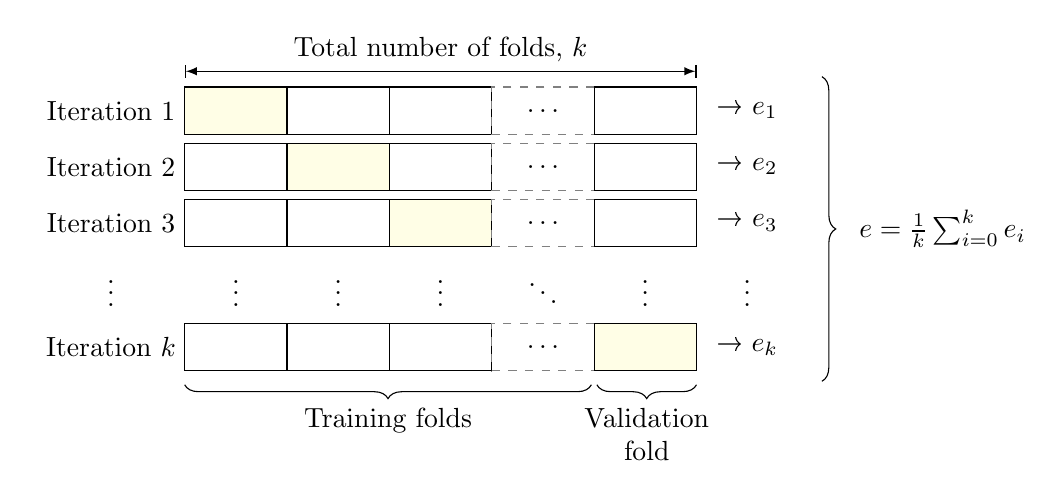
\begin{tikzpicture}
    \matrix (M)
        [
        matrix of nodes,
        nodes={
            minimum height = 6mm,
            minimum width = 1.3cm,
            outer sep=0,
            anchor=center,
            draw
        },
        column 1/.style={nodes={draw=none}, minimum width = 4cm},
        column 5/.style={nodes={draw=gray}, dashed},
        column 7/.style={nodes={draw=none},minimum width = 1.0cm},
        row 4/.style={nodes={draw=none}},
        row sep=1mm,
        column sep=-\pgflinewidth,
        nodes in empty cells,
        e/.style={fill=yellow!10},
        n/.style={nodes={draw=none, fill=none}},
        ]
    {
        Iteration 1   & |[e]|  &        &        & $\ldots$ &        & \textrightarrow\;$e_1$ \\
        Iteration 2   &        & |[e]|  &        & $\ldots$ &        & \textrightarrow\;$e_2$ \\
        Iteration 3   &        &        & |[e]|  & $\ldots$ &        & \textrightarrow\;$e_3$ \\
              $\vdots$  & $\vdots$ & $\vdots$ & $\vdots$ & $\ddots$ & $\vdots$ & $\vdots$                \\
        Iteration $k$ &        &        &        & $\ldots$ & |[e]|  & \textrightarrow\;$e_k$ \\
    };
    \draw (M-1-2.north west) ++(0,2mm) coordinate (LT) edge[|<->|, >= latex] node[above]{Total number of folds, $k$} (LT-|M-1-6.north east);
%    \draw[decorate,decoration = {brace}] (bias-brace-down) --  (bias-brace-up);
    \draw[decorate,decoration = {brace, raise=0.5em, amplitude=0.5em}]
        (M-5-6.south east)
        -- node[below=1em, align=center] {Validation \\ fold}
        ([shift={(0.1em,0)}]M-5-6.south west);

    \draw[decorate,decoration = {brace, raise=0.5em, amplitude=0.5em}]
        ([shift={(-0.1em,0)}]M-5-5.south east)
        -- node[below=1em, align=center] {Training folds}
        (M-5-2.south west);

    \draw[decorate,decoration = {brace, raise=0.5em, amplitude=0.5em}]
        (M.north east)
        -- node[midway, right=1.5em] {$e=\frac{1}{k}\sum_{i=0}^k{e_i}$}
        (M.south east);

%    \matrix (L)
%        [
%        matrix of nodes,
%        right=of M,
%        nodes={
%            minimum height = 6mm,
%            minimum width = 1.5cm,
%            outer sep=0,
%            anchor=center,
%            draw
%        },
%        column 1/.style={nodes={draw=none}, minimum width = 4cm},
%        row sep=1mm,
%        column sep=-\pgflinewidth,
%        nodes in empty cells,
%        e/.style={fill=yellow!10}
%        ]
%    {
%        Training   &       \\
%        Validation & |[e]| \\
%    };

%    \node[east=of M.east] {
%    \hskip1em
%    \begin{tabular}[c]{|p{2em}|l}
%      \cline{1-1}
%      \ccell{0}{1}  & Training
%      \nextrow{1-1}
%      \ccell{1}{1}  & Validation\\
%      \cline{1-1}
%    \end{tabular}
%    }
\end{tikzpicture}
    \captionsetup{format=hang} % hanging captions
    \caption{
        $k$-fold cross-validation procedure: (1) Dataset is divided into
        $k$-folds of roughly equal size. (2) Choose one fold randomly to be the
        holdout set then fit model on the remaining $k-1$ folds. (3) Iterate
        through the remaining $k-1$ folds, using each as the holdout set and
        record the error $e_i$ of the iteration. (4) Average the errors obtained
        over the $k$-folds.
    }
    \label{fig:kfold-cv}
\end{figure}

%\subsubsection{Leave-One-Out Cross-Validation (LOOCV)}
%%%%%%%%%%%%%%%%%%%%%%%%%%%%%%%%%%%%%%%%%%%%%%%%%%%%%%%%%%%%%%%%%%%%%%%%%%%%%%%%

%\subsubsection{Bootstrapping}
%%%%%%%%%%%%%%%%%%%%%%%%%%%%%%%%%%%%%%%%%%%%%%%%%%%%%%%%%%%%%%%%%%%%%%%%%%%%%%%%

%\subsection{Supervised}
%%%%%%%%%%%%%%%%%%%%%%%%%%%%%%%%%%%%%%%%%%%%%%%%%%%%%%%%%%%%%%%%%%%%%%%%%%%%%%%%


\section{Deep Learning\label{sec:DL}}
%%%%%%%%%%%%%%%%%%%%%%%%%%%%%%%%%%%%%%%%%%%%%%%%%%%%%%%%%%%%%%%%%%%%%%%%%%%%%%%%
\Gls{DL} is a field of \gls{ML} that is primarily concerned with
the learning of representations of data. The main idea is to use a \gls{NN} to learn representations of data. The main difference between a
\gls{NN} and a traditional \gls{ML} algorithm is that the
neural network is a function of the data, rather than the data itself.

\subsection{The fundamental component: Perceptrons}
%%%%%%%%%%%%%%%%%%%%%%%%%%%%%%%%%%%%%%%%%%%%%%%%%%%%%%%%%%%%%%%%%%%%%%%%%%%%%%%%

Proposed by Rosenblatt \cite{Rosenblatt_1957_6098} in his technical
report funded by the United States Office of Naval Research
\cite{doi:10.1177/030631296026003005} in 1957, the \textit{perceptron} is a
fundamental component of deep learning, describing a mathematical model of a
biological neuron. There are two different sets of notation which exist when
dealing with the bias of a perceptron. One involves the inclusion of a unit
constant in the input vector $\mathbf{x}$, with the bias being specified by the
value of the first weight $w_0$. An alternative notation exists which treats the
bias as a standalone value $b$. The latter notation will be used, as it is the
preferred notation in contemporary deep learning papers. The notation defining
the mapping of a perceptron is then: $f(\mathbf{x};\mathbf{w},
b)=\mathbf{x}^T\mathbf{w}+b$; $x\in\mathbb{R}^{d_{in}}$,
$\mathbf{w}\in\mathbb{R}^{d_{in}}$, $b\in\mathbb{R}$.

\begin{figure}[htbp]
    \centering
    % MIT License
%
% Copyright (c) 2021 Geoffrey H. Garrett
%
% Permission is hereby granted, free of charge, to any person obtaining a copy
% of this software and associated documentation files (the "Software"), to deal
% in the Software without restriction, including without limitation the rights
% to use, copy, modify, merge, publish, distribute, sublicense, and/or sell
% copies of the Software, and to permit persons to whom the Software is
% furnished to do so, subject to the following conditions:
%
% The above copyright notice and this permission notice shall be included in all
% copies or substantial portions of the Software.
%
% THE SOFTWARE IS PROVIDED "AS IS", WITHOUT WARRANTY OF ANY KIND, EXPRESS OR
% IMPLIED, INCLUDING BUT NOT LIMITED TO THE WARRANTIES OF MERCHANTABILITY,
% FITNESS FOR A PARTICULAR PURPOSE AND NONINFRINGEMENT. IN NO EVENT SHALL THE
% AUTHORS OR COPYRIGHT HOLDERS BE LIABLE FOR ANY CLAIM, DAMAGES OR OTHER
% LIABILITY, WHETHER IN AN ACTION OF CONTRACT, TORT OR OTHERWISE, ARISING FROM,
% OUT OF OR IN CONNECTION WITH THE SOFTWARE OR THE USE OR OTHER DEALINGS IN THE
% SOFTWARE.

%%%%%%%%%%%%%%%%%%%%%%%%%%%%%%%%%%%%%%%%%%%%%%%%%%%%%%%%%%%%%%%%%%%%%%%%%%%%%%%
% ACKNOWLEDGEMENTS
%%%%%%%%%%%%%%%%%%%%%%%%%%%%%%%%%%%%%%%%%%%%%%%%%%%%%%%%%%%%%%%%%%%%%%%%%%%%%%%
% Design and implementation of this diagram was inspired and adapted from:
% https://tex.stackexchange.com/questions/104334/tikz-diagram-of-a-perceptron

%%%%%%%%%%%%%%%%%%%%%%%%%%%%%%%%%%%%%%%%%%%%%%%%%%%%%%%%%%%%%%%%%%%%%%%%%%%%%%%
% DEPENDENCIES
%%%%%%%%%%%%%%%%%%%%%%%%%%%%%%%%%%%%%%%%%%%%%%%%%%%%%%%%%%%%%%%%%%%%%%%%%%%%%%%
%\usepackage{tikz}
%\usetikzlibrary{decorations.pathreplacing}    % for TikZ braces
%\usetikzlibrary{positioning}                  % for TikZ relative positioning

%%%%%%%%%%%%%%%%%%%%%%%%%%%%%%%%%%%%%%%%%%%%%%%%%%%%%%%%%%%%%%%%%%%%%%%%%%%%%%%
% USER STYLING
%%%%%%%%%%%%%%%%%%%%%%%%%%%%%%%%%%%%%%%%%%%%%%%%%%%%%%%%%%%%%%%%%%%%%%%%%%%%%%%

% TikZ node design.
\tikzset{basic/.style={draw,text width=1em,text badly centered}}
\tikzset{input/.style={}}
\tikzset{output/.style={}}
\tikzset{weight/.style={basic,circle}}
\tikzset{hidden/.style={basic,circle}}
\tikzset{function/.style={basic,circle}}

% Labels and symbols.
\def\activationlabel{activation function}  % activation function label
\def\activationsymbol{$\phi$}              % activation function symbol
\def\transferlabel{transfer function}      % transfer function label
\def\transfersymbol{$\sum$}                % transfer function symbol
\def\outputsymbol{$y$}                     % output symbol
\def\inputsymbol{$x$}                      % input symbol
\def\inputvecsymbol{$\mathbf{x}$}          % input vector symbol
\def\weightslabel{weights}                 % input vector symbol
\def\biassymbol{$b$}                       % bias symbol

%%%%%%%%%%%%%%%%%%%%%%%%%%%%%%%%%%%%%%%%%%%%%%%%%%%%%%%%%%%%%%%%%%%%%%%%%%%%%%%
% TIKZ PICTURE
%%%%%%%%%%%%%%%%%%%%%%%%%%%%%%%%%%%%%%%%%%%%%%%%%%%%%%%%%%%%%%%%%%%%%%%%%%%%%%%
\begin{tikzpicture}
    \usetikzlibrary{decorations.pathreplacing}    % for TikZ braces
    \usetikzlibrary{positioning}                  % for TikZ relative positioning

    \node[function] at (\transferx, -{int(2)})  (transfer) {\transfersymbol};
    \node[function, right=3em of transfer] (activation) {\activationsymbol};
    \node[below of=activation,font=\scriptsize,text width=3em] {\activationlabel};
    \node[below of=transfer,font=\scriptsize,text width=3em] {\transferlabel};
    \node[output, right=\layersep of activation] (output) {\outputsymbol};
    \path[draw,->] (transfer) -- (activation);
    \path[draw,->] (activation) -- (output);

    % Iterate through each row of units.
    \foreach \n [evaluate=\n as \p using {int(\n-1)}] in {0,1,2,3,4} {
        \ifnum \n=0
        \node[input] at (0, -\n) (X-\n) {$1$};
        \node[weight] at (\layersep, -\n) (W-\n) {$w_\n$};
        \else \ifnum \n=3
        \node[] at (0, -\n) (X-\n) {$\vdots$};
        \node[] at (\layersep, -\n) (W-\n) {$\vdots$};
        \else \ifnum \n=4
        \node[input] at (0, -\n) (X-\n) {$x_{d_{{in}}}$};
        \node[weight,label={[xshift=-0.0em]center:$w_{d_{{in}}}$}] at (\layersep, -\n) (W-\n) {\phantom{$w_{d_{{in}}}$}};
        \else
        \node[input] at (0, -\n) (X-\n) {$x_\n$};
        \node[weight] at (\layersep, -\n) (W-\n) {$w_\n$};
        \fi
        \fi
        \fi

        % Arrow from input to weight.
        \ifnum \n=3
        \else
        \path[draw,->] (X-\n) -- (W-\n);
                    \path[draw,->] (W-\n) -- (transfer);
        \fi

    }

    % Brace for bias.
    \node[left=1em of X-0] (bias-brace) {};
    \node[above=1em of bias-brace] (bias-brace-up) {};
    \node[below=1em of bias-brace] (bias-brace-down) {};
    \draw[decorate,decoration = {brace}] (bias-brace-down) --  (bias-brace-up);
    \node[left of=bias-brace,font=\scriptsize] {bias, \biassymbol};

    % Brace for input.
    \node[below=10em of bias-brace-down] (input-brace-down) {};
    \node[below=5em of bias-brace-down] (input-brace) {};
    \draw[decorate,decoration = {brace}] (input-brace-down) --  (bias-brace-down);
    \node[left of=input-brace,font=\scriptsize] {inputs, \inputvecsymbol};

    % Weights label.
    \node[below of=W-4,font=\scriptsize] {\weightslabel};

\end{tikzpicture}

    \caption{Perceptron}
    \label{fig:perceptron}
\end{figure}

This mathematical mimicry of a biological neuron was first used used proposed by
Rosenblatt where a set of inputs $\mathbf{x}$ weighted using $\mathbf{w}$ before
being summed. If this sum surpassed a threshold, then a binary output of $1$ was
returned. \autoref{fig:perceptron} shows a more general formulation which
applies to the resulting field of deep learning, with any activation function
$\phi$ analogous for the level of excitation of a biological neuron in response
to its stimulus $\mathbf{x}$.

The primary criticism of the perceptron came in 1969 from Minsky and Papert
\cite{minsky69perceptrons}, where it was shown that the perceptron could only
solve \textit{linearly separable} functions, and failed to solve the XOR and
NXOR functions. They went on to claim that the research being done was doomed to
failure due to these limitations, resulting in little research in the area being
done until about the 1980's.

\subsection{Activation function}
%%%%%%%%%%%%%%%%%%%%%%%%%%%%%%%%%%%%%%%%%%%%%%%%%%%%%%%%%%%%%%%%%%%%%%%%%%%%%%%%

Since the early days of the perceptron, a wide variety of activation functions
$\phi$ have been used and improve upon the threshold step function.

%\begin{figure}[htbp]
%    \centering
%    \makeatletter
\pgfmathdeclarefunction{erf}{1}{%
    \begingroup
    \pgfmathparse{#1 > 0 ? 1 : -1}%
    \edef\sign{\pgfmathresult}%
    \pgfmathparse{abs(#1)}%
    \edef\x{\pgfmathresult}%
    \pgfmathparse{1/(1+0.3275911*\x)}%
    \edef\t{\pgfmathresult}%
    \pgfmathparse{%
        1 - (((((1.061405429*\t -1.453152027)*\t) + 1.421413741)*\t
        -0.284496736)*\t + 0.254829592)*\t*exp(-(\x*\x))}%
    \edef\y{\pgfmathresult}%
    \pgfmathparse{(\sign)*\y}%
    \pgfmath@smuggleone\pgfmathresult%
    \endgroup
}
%dep
%subfig
\begin{figure}[htp]
    \centering
    \captionsetup{format=hang} % hanging captions
    \subfloat[Threshold Step]{
        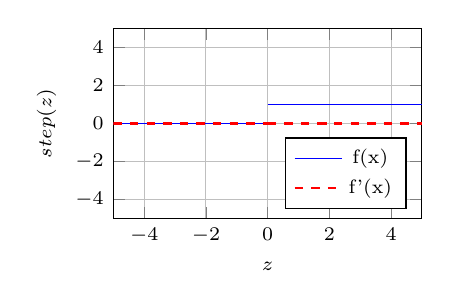
\begin{tikzpicture}
            \label{fig:threshold}
            \begin{axis}
                [width=5.5cm,height=4cm,ylabel=$step(z)$,xlabel=$z$,ymin=-5.0,ymax=5.0,xmin=-5,xmax=5,
                legend style={at={(0.95,0.05)},anchor=south east},]
                \addplot[blue,smooth, domain=-5:0] {0};
                \addplot[red,dashed, thick, domain=-5:0] {0};
                \addplot[blue,smooth, domain=-0:5] {1};
                \addplot[red,dashed, thick, domain=-0:5] {0};
                \addlegendentry{f(x)}
                \addlegendentry{f'(x)}
            \end{axis}
        \end{tikzpicture}
    }
    \subfloat[Linear]{
        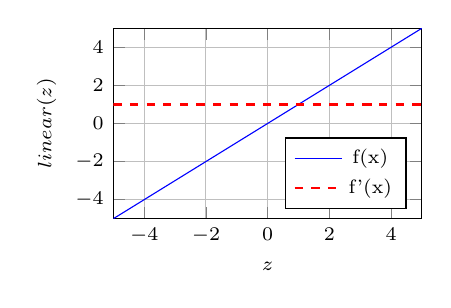
\begin{tikzpicture}
            \label{fig:linear}
            \begin{axis}
                [width=5.5cm,height=4cm,ylabel=$linear(z)$,xlabel=$z$,ymin=-5.0,ymax=5.0,xmin=-5,xmax=5,
                legend style={at={(0.95,0.05)},anchor=south east},]
                \addplot[blue,smooth] {x};
                \addlegendentry{f(x)}
                \addplot[red,dashed, thick] {1};
                \addlegendentry{f'(x)}
            \end{axis}
        \end{tikzpicture}
    }
    \subfloat[Sigmoid]{
        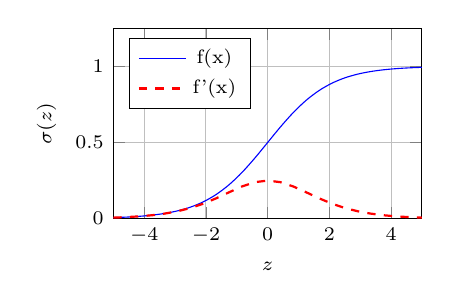
\begin{tikzpicture}
            \label{fig:sigmoid}
            \begin{axis}
                [width=5.5cm,height=4cm,ylabel=$\sigma(z)$,xlabel=$z$,ymin=0,ymax=1.25,xmin=-5,xmax=5,
                legend style={at={(0.05,0.95)},anchor=north west},]
                \addplot[blue,smooth] {1/(1+exp(-x))};
                \addlegendentry{f(x)}
                \addplot[red, dashed, thick] {1/(1+exp(-x)) * (1-1/(1+exp(-x)))};
                \addlegendentry{f'(x)}
            \end{axis}
        \end{tikzpicture}
    }\\
    \subfloat[Hyperbolic tangent]{
        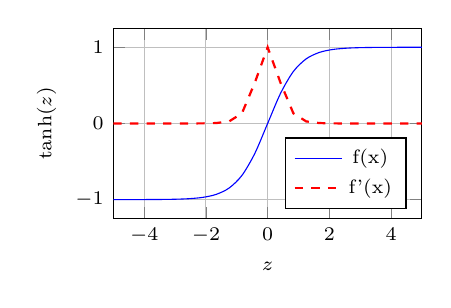
\begin{tikzpicture}
            \label{fig:hyperbolic_tangent}
            \begin{axis}
                [width=5.5cm,height=4cm,ylabel=$\tanh(z)$,xlabel=$z$,ymin=-1.25,ymax=1.25,xmin=-5,xmax=5, legend style={at={(0.95,0.05)},anchor=south east},]
                \addplot[blue,smooth] {tanh(x)};
                \addlegendentry{f(x)}
                \addplot[red,dashed, thick] {1/cosh(2*x)*1/cosh(2*x)};
                \addlegendentry{f'(x)}
            \end{axis}
        \end{tikzpicture}
    }
    \subfloat[ReLU]{
        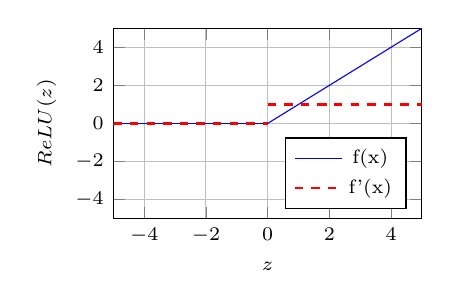
\begin{tikzpicture}
            \label{fig:relu}
            \begin{axis}
                [width=5.5cm,height=4cm,ylabel=$ReLU(z)$,xlabel=$z$,ymin=-5.0,ymax=5.0,xmin=-5,xmax=5,
                legend style={at={(0.95,0.05)},anchor=south east},]
                \addplot[blue,smooth, domain=-5:0] {0};
                \addplot[red,dashed, thick, domain=-5:0] {0};
                \addplot[blue,smooth, domain=-0:5] {x};
                \addplot[red,dashed, thick, domain=-0:5] {1};
                \addlegendentry{f(x)}
                \addlegendentry{f'(x)}
            \end{axis}
        \end{tikzpicture}
    }
    \subfloat[Leaky ReLU]{
        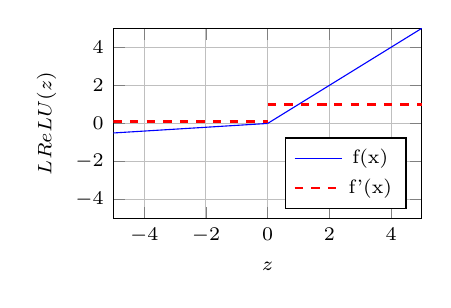
\begin{tikzpicture}
            \label{fig:lrelu}
            \begin{axis}
                [width=5.5cm,height=4cm,ylabel=$LReLU(z)$,xlabel=$z$,ymin=-5.0,ymax=5.0,xmin=-5,xmax=5,
                legend style={at={(0.95,0.05)},anchor=south east},]
                \addplot[blue,smooth, domain=-5:0] {0.1*x};
                \addplot[red,dashed, thick, domain=-5:0] {0.1};
                \addplot[blue,smooth, domain=-0:5] {x};
                \addplot[red,dashed, thick, domain=-0:5] {1};
                \addlegendentry{f(x)}
                \addlegendentry{f'(x)}
            \end{axis}
        \end{tikzpicture}
    }\\
    \subfloat[GELU]{
        \begin{tikzpicture}
            \label{fig:gelu}
            \begin{axis}
                [width=5.5cm,height=4cm,ylabel=$GELU(z)$,xlabel=$z$,ymin=-5.0,ymax=5.0,xmin=-5,xmax=5,
                legend style={at={(0.95,0.05)},anchor=south east},]
                \addplot[blue,smooth] {x * 0.5 * (1 + erf(x /sqrt(2)))};
                \addplot[red,dashed, thick] {0.5 * (1 + erf(x /sqrt(2))) + 1/sqrt(2*pi) * (exp(-x*x/2))};
                \addlegendentry{f(x)}
                \addlegendentry{f'(x)}
            \end{axis}
        \end{tikzpicture}
    }
    \subfloat[Swish]{
        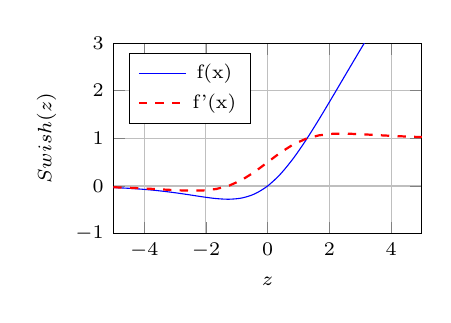
\begin{tikzpicture}
            \label{fig:swish}
            \begin{axis}
                [width=5.5cm,height=4cm,ylabel=$Swish(z)$,xlabel=$z$,ymin=-1,ymax=3.0,xmin=-5,xmax=5,
                legend style={at={(0.05,0.95)},anchor=north west},]
                \addplot[blue,smooth] {x*(1/(1+exp(-x)))}; % f (x) + σ (x) (1 − f (x))
                \addlegendentry{f(x)}
                \addplot[red, dashed, thick] {x/(1+exp(-x)) + 1/(1+exp(-x)) * (1-x/(1+exp(-x)))};
                \addlegendentry{f'(x)}
            \end{axis}
        \end{tikzpicture}
    }
    \subfloat[SIREN]{
        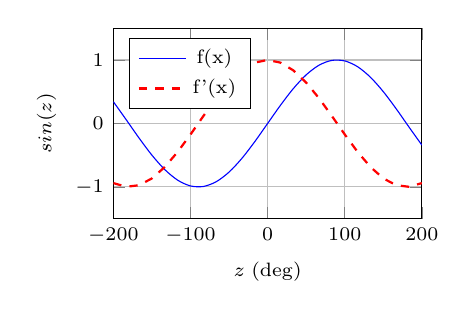
\begin{tikzpicture}
            \label{fig:siren}
            \begin{axis}
                [width=5.5cm,height=4cm,ylabel=$sin(z)$,xlabel=$z\;\text{(deg)}$,ymin=-1.5,ymax=1.5,xmin=-200,xmax=200,
                legend style={at={(0.05,0.95)},anchor=north west},]
                \addplot[blue,smooth,domain=-200:200] {sin(x)}; % f (x) + σ (x) (1 − f (x))
                \addlegendentry{f(x)}
                \addplot[red, dashed, thick,domain=-200:200] {cos(x)};
                \addlegendentry{f'(x)}
            \end{axis}
        \end{tikzpicture}
    }
    \caption[Activation functions.]{\textbf{Activation functions} used in \gls{DL}, included for results in their performance or historic significance in the applications of artificial neural networks.}
    \label{fig:activation-functions}
\end{figure}
%    \caption{Activation functions}
%    \label{fig:activation}
%\end{figure}
\makeatletter
\pgfmathdeclarefunction{erf}{1}{%
    \begingroup
    \pgfmathparse{#1 > 0 ? 1 : -1}%
    \edef\sign{\pgfmathresult}%
    \pgfmathparse{abs(#1)}%
    \edef\x{\pgfmathresult}%
    \pgfmathparse{1/(1+0.3275911*\x)}%
    \edef\t{\pgfmathresult}%
    \pgfmathparse{%
        1 - (((((1.061405429*\t -1.453152027)*\t) + 1.421413741)*\t
        -0.284496736)*\t + 0.254829592)*\t*exp(-(\x*\x))}%
    \edef\y{\pgfmathresult}%
    \pgfmathparse{(\sign)*\y}%
    \pgfmath@smuggleone\pgfmathresult%
    \endgroup
}
%dep
%subfig
\begin{figure}[htp]
    \centering
    \captionsetup{format=hang} % hanging captions
    \subfloat[Threshold Step]{
        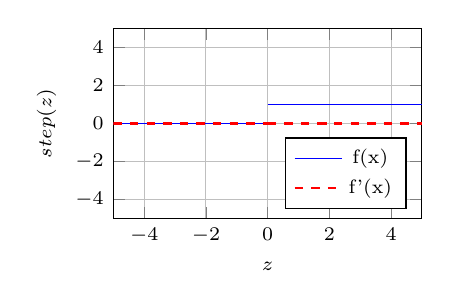
\begin{tikzpicture}
            \label{fig:threshold}
            \begin{axis}
                [width=5.5cm,height=4cm,ylabel=$step(z)$,xlabel=$z$,ymin=-5.0,ymax=5.0,xmin=-5,xmax=5,
                legend style={at={(0.95,0.05)},anchor=south east},]
                \addplot[blue,smooth, domain=-5:0] {0};
                \addplot[red,dashed, thick, domain=-5:0] {0};
                \addplot[blue,smooth, domain=-0:5] {1};
                \addplot[red,dashed, thick, domain=-0:5] {0};
                \addlegendentry{f(x)}
                \addlegendentry{f'(x)}
            \end{axis}
        \end{tikzpicture}
    }
    \subfloat[Linear]{
        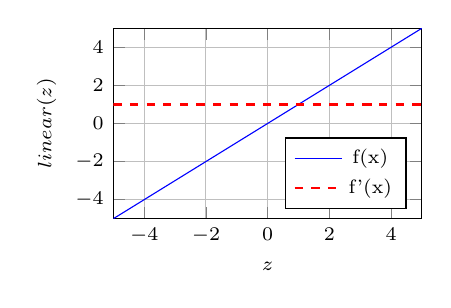
\begin{tikzpicture}
            \label{fig:linear}
            \begin{axis}
                [width=5.5cm,height=4cm,ylabel=$linear(z)$,xlabel=$z$,ymin=-5.0,ymax=5.0,xmin=-5,xmax=5,
                legend style={at={(0.95,0.05)},anchor=south east},]
                \addplot[blue,smooth] {x};
                \addlegendentry{f(x)}
                \addplot[red,dashed, thick] {1};
                \addlegendentry{f'(x)}
            \end{axis}
        \end{tikzpicture}
    }
    \subfloat[Sigmoid]{
        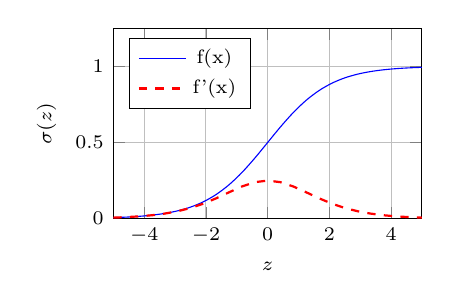
\begin{tikzpicture}
            \label{fig:sigmoid}
            \begin{axis}
                [width=5.5cm,height=4cm,ylabel=$\sigma(z)$,xlabel=$z$,ymin=0,ymax=1.25,xmin=-5,xmax=5,
                legend style={at={(0.05,0.95)},anchor=north west},]
                \addplot[blue,smooth] {1/(1+exp(-x))};
                \addlegendentry{f(x)}
                \addplot[red, dashed, thick] {1/(1+exp(-x)) * (1-1/(1+exp(-x)))};
                \addlegendentry{f'(x)}
            \end{axis}
        \end{tikzpicture}
    }\\
    \subfloat[Hyperbolic tangent]{
        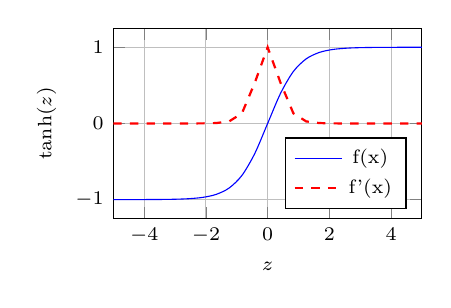
\begin{tikzpicture}
            \label{fig:hyperbolic_tangent}
            \begin{axis}
                [width=5.5cm,height=4cm,ylabel=$\tanh(z)$,xlabel=$z$,ymin=-1.25,ymax=1.25,xmin=-5,xmax=5, legend style={at={(0.95,0.05)},anchor=south east},]
                \addplot[blue,smooth] {tanh(x)};
                \addlegendentry{f(x)}
                \addplot[red,dashed, thick] {1/cosh(2*x)*1/cosh(2*x)};
                \addlegendentry{f'(x)}
            \end{axis}
        \end{tikzpicture}
    }
    \subfloat[ReLU]{
        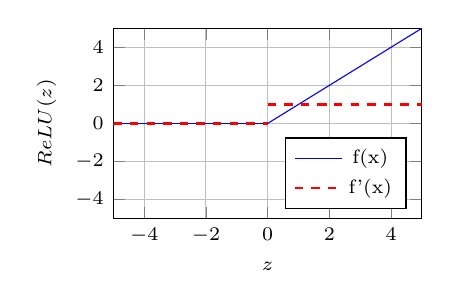
\begin{tikzpicture}
            \label{fig:relu}
            \begin{axis}
                [width=5.5cm,height=4cm,ylabel=$ReLU(z)$,xlabel=$z$,ymin=-5.0,ymax=5.0,xmin=-5,xmax=5,
                legend style={at={(0.95,0.05)},anchor=south east},]
                \addplot[blue,smooth, domain=-5:0] {0};
                \addplot[red,dashed, thick, domain=-5:0] {0};
                \addplot[blue,smooth, domain=-0:5] {x};
                \addplot[red,dashed, thick, domain=-0:5] {1};
                \addlegendentry{f(x)}
                \addlegendentry{f'(x)}
            \end{axis}
        \end{tikzpicture}
    }
    \subfloat[Leaky ReLU]{
        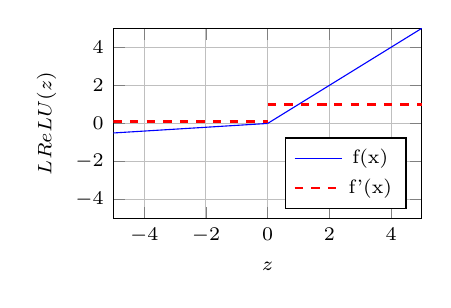
\begin{tikzpicture}
            \label{fig:lrelu}
            \begin{axis}
                [width=5.5cm,height=4cm,ylabel=$LReLU(z)$,xlabel=$z$,ymin=-5.0,ymax=5.0,xmin=-5,xmax=5,
                legend style={at={(0.95,0.05)},anchor=south east},]
                \addplot[blue,smooth, domain=-5:0] {0.1*x};
                \addplot[red,dashed, thick, domain=-5:0] {0.1};
                \addplot[blue,smooth, domain=-0:5] {x};
                \addplot[red,dashed, thick, domain=-0:5] {1};
                \addlegendentry{f(x)}
                \addlegendentry{f'(x)}
            \end{axis}
        \end{tikzpicture}
    }\\
    \subfloat[GELU]{
        \begin{tikzpicture}
            \label{fig:gelu}
            \begin{axis}
                [width=5.5cm,height=4cm,ylabel=$GELU(z)$,xlabel=$z$,ymin=-5.0,ymax=5.0,xmin=-5,xmax=5,
                legend style={at={(0.95,0.05)},anchor=south east},]
                \addplot[blue,smooth] {x * 0.5 * (1 + erf(x /sqrt(2)))};
                \addplot[red,dashed, thick] {0.5 * (1 + erf(x /sqrt(2))) + 1/sqrt(2*pi) * (exp(-x*x/2))};
                \addlegendentry{f(x)}
                \addlegendentry{f'(x)}
            \end{axis}
        \end{tikzpicture}
    }
    \subfloat[Swish]{
        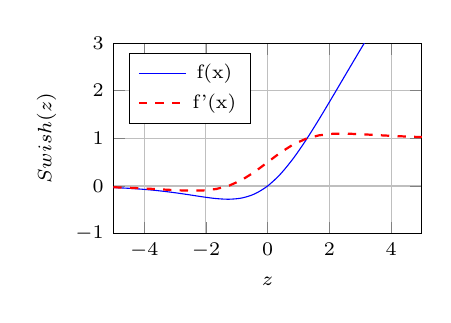
\begin{tikzpicture}
            \label{fig:swish}
            \begin{axis}
                [width=5.5cm,height=4cm,ylabel=$Swish(z)$,xlabel=$z$,ymin=-1,ymax=3.0,xmin=-5,xmax=5,
                legend style={at={(0.05,0.95)},anchor=north west},]
                \addplot[blue,smooth] {x*(1/(1+exp(-x)))}; % f (x) + σ (x) (1 − f (x))
                \addlegendentry{f(x)}
                \addplot[red, dashed, thick] {x/(1+exp(-x)) + 1/(1+exp(-x)) * (1-x/(1+exp(-x)))};
                \addlegendentry{f'(x)}
            \end{axis}
        \end{tikzpicture}
    }
    \subfloat[SIREN]{
        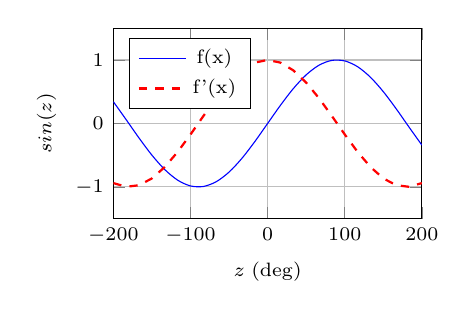
\begin{tikzpicture}
            \label{fig:siren}
            \begin{axis}
                [width=5.5cm,height=4cm,ylabel=$sin(z)$,xlabel=$z\;\text{(deg)}$,ymin=-1.5,ymax=1.5,xmin=-200,xmax=200,
                legend style={at={(0.05,0.95)},anchor=north west},]
                \addplot[blue,smooth,domain=-200:200] {sin(x)}; % f (x) + σ (x) (1 − f (x))
                \addlegendentry{f(x)}
                \addplot[red, dashed, thick,domain=-200:200] {cos(x)};
                \addlegendentry{f'(x)}
            \end{axis}
        \end{tikzpicture}
    }
    \caption[Activation functions.]{\textbf{Activation functions} used in \gls{DL}, included for results in their performance or historic significance in the applications of artificial neural networks.}
    \label{fig:activation-functions}
\end{figure}

\subsection{Multilayer perceptrons, a.k.a feed forward networks}
%%%%%%%%%%%%%%%%%%%%%%%%%%%%%%%%%%%%%%%%%%%%%%%%%%%%%%%%%%%%%%%%%%%%%%%%%%%%%%%%

$f(\mathbf{x};\mathbf{w}, b)=\mathbf{x}^T\mathbf{w}+b$; $x\in\mathbb{R}^{d_{in}}$, $\mathbf{w}\in\mathbb{R}^{d_{in}\times}$, $b\in\mathbb{R}^1$.

\begin{figure}
    \centering
    % MIT License
%
% Copyright (c) 2021 Geoffrey H. Garrett
%
% Permission is hereby granted, free of charge, to any person obtaining a copy
% of this software and associated documentation files (the "Software"), to deal
% in the Software without restriction, including without limitation the rights
% to use, copy, modify, merge, publish, distribute, sublicense, and/or sell
% copies of the Software, and to permit persons to whom the Software is
% furnished to do so, subject to the following conditions:
%
% The above copyright notice and this permission notice shall be included in all
% copies or substantial portions of the Software.
%
% THE SOFTWARE IS PROVIDED "AS IS", WITHOUT WARRANTY OF ANY KIND, EXPRESS OR
% IMPLIED, INCLUDING BUT NOT LIMITED TO THE WARRANTIES OF MERCHANTABILITY,
% FITNESS FOR A PARTICULAR PURPOSE AND NONINFRINGEMENT. IN NO EVENT SHALL THE
% AUTHORS OR COPYRIGHT HOLDERS BE LIABLE FOR ANY CLAIM, DAMAGES OR OTHER
% LIABILITY, WHETHER IN AN ACTION OF CONTRACT, TORT OR OTHERWISE, ARISING FROM,
% OUT OF OR IN CONNECTION WITH THE SOFTWARE OR THE USE OR OTHER DEALINGS IN THE
% SOFTWARE.

%%%%%%%%%%%%%%%%%%%%%%%%%%%%%%%%%%%%%%%%%%%%%%%%%%%%%%%%%%%%%%%%%%%%%%%%%%%%%%%
% ACKNOWLEDGEMENTS
%%%%%%%%%%%%%%%%%%%%%%%%%%%%%%%%%%%%%%%%%%%%%%%%%%%%%%%%%%%%%%%%%%%%%%%%%%%%%%%
% Adapted from:
% https://www.researchgate.net/figure/The-agent-environment-interaction-in-reinforcement-learning_fig1_328494763

%%%%%%%%%%%%%%%%%%%%%%%%%%%%%%%%%%%%%%%%%%%%%%%%%%%%%%%%%%%%%%%%%%%%%%%%%%%%%%%
% DEPENDENCIES
%%%%%%%%%%%%%%%%%%%%%%%%%%%%%%%%%%%%%%%%%%%%%%%%%%%%%%%%%%%%%%%%%%%%%%%%%%%%%%%
%\usepackage{tikz}
%\usetikzlibrary{decorations.pathreplacing}    % for TikZ braces
%\usetikzlibrary{positioning}                  % for TikZ relative positioning

%%%%%%%%%%%%%%%%%%%%%%%%%%%%%%%%%%%%%%%%%%%%%%%%%%%%%%%%%%%%%%%%%%%%%%%%%%%%%%%
% USER STYLING
%%%%%%%%%%%%%%%%%%%%%%%%%%%%%%%%%%%%%%%%%%%%%%%%%%%%%%%%%%%%%%%%%%%%%%%%%%%%%%%

% TikZ node design.
\tikzset{basic/.style={draw,text width=1em,text badly centered}}
\tikzset{input/.style={basic, fill=green!25, circle}}
\tikzset{output/.style={basic, fill=blue!25, circle}}
\tikzset{weight/.style={basic,circle}}
\tikzset{hidden/.style={basic,circle}}
\tikzset{function/.style={basic,circle}}
\def\layersep{3em}
\def\transferx{9em}
\def\hiddenx{7em}
\def\hiddenxn{12em}


\def\sep{4em}
\def\L{\gls{L}}       % number of hidden layers
\def\y{\gls{y_true}}  % output vector
\def\x{\gls{ml:x}}    % input vector
\def\h{\gls{a_vec}}   % hidden output
\def\nx{\gls{ml:n_x}}   % hidden output
\def\ny{\gls{ml:n_y}}   % hidden output


%%%%%%%%%%%%%%%%%%%%%%%%%%%%%%%%%%%%%%%%%%%%%%%%%%%%%%%%%%%%%%%%%%%%%%%%%%%%%%%
% TIKZ PICTURE
%%%%%%%%%%%%%%%%%%%%%%%%%%%%%%%%%%%%%%%%%%%%%%%%%%%%%%%%%%%%%%%%%%%%%%%%%%%%%%%
\begin{tikzpicture}
    \usetikzlibrary{decorations.pathreplacing}    % for TikZ braces
    \usetikzlibrary{positioning}                  % for TikZ relative positioning

    % input
    \foreach \n/\p in {0/1,1/2,2/3,3/4,4/5} {
        \ifnum \n=3
            % dots layer
            \node[] at (0, -\n) (X_\n) {$\vdots$};
            \node[] at (\hiddenx, -\n) (H1_\n) {$\vdots$};
            \node[right of=H1_\n] (M-\n) {$\ddots$};
            \node[below of=H1_2] (H2_\n) {$\vdots$};
            \node[below of=H2_2] (H2_\n) {$\vdots$};
            \node[right=5.7em of H2_\n] (Y_\n) {$\vdots$};
        \else
        \ifnum \n=4
            % n layer
            \node[input] at (0, -\n) (X_\n) {};
            \node[left of=X_\n] (I_\n) {$x_{\nx}$};
            \path[draw,->] (I_\n) -- (X_\n);
            \node[hidden] at (\hiddenx, -\n) (H1_\n) {}; %{$h_{n, 1}$};
            \node[right of= H1_\n] (M-\n) {$\ldots$};
            \node[hidden, right of= M-\n] (H2_\n) {}; % {$h_{n, m}$};
            \node[output, right= 5em of H2_\n] (Y_\n) {}; % {$h_{n, m}$};
            \node[right of=Y_\n] (O_\n) {$y_{\ny}$};
            \path[draw,->] (Y_\n) -- (O_\n);
        \else
            \node[input] at (0, -{\n}) (X_\n) {};
            \node[left of=X_\n] (I_\n) {$x_{\p}$};
            \path[draw,->] (I_\n) -- (X_\n);
            \node[hidden] at (\hiddenx, -\n) (H1_\n) {};%{$h_{\n, 1}$};
            \node[right of=H1_\n] (M-\n) {$\ldots$};
            \node[hidden, right of=M-\n] (H2_\n) {};% {$h_{\n, m}$};
            \node[output, right= 5em of H2_\n] (Y_\n) {}; % {$h_{n, m}$};
            \node[right of=Y_\n] (O_\n) {$y_\p$};
            \path[draw,->] (Y_\n) -- (O_\n);
        \fi
        \fi
    }

    % input layer connected to first hidden layer
    \foreach \j in {0,1,2,4} {
        \foreach \n in {0,1,2,4} {
            \path[draw,->] (X_\n) -- (H1_\j);
        }
    }

    % second hidden layer connected to output layer
    \foreach \j in {0,1,2,4} {
        \foreach \n in {0,1,2,4} {
            \path[draw,->] (H2_\n) -- (Y_\j);
        }
    }

    % labels
    \node[below of=X_4,font=\scriptsize, align=center] {input\\layer};
    \node[below of=Y_4,font=\scriptsize, align=center] {output\\layer};

    % brace for hidden layers
    \node[below=1em of M-4] (hidden-brace) {};
    \node[right=3em of hidden-brace] (hidden-brace-right) {};
    \node[left=3em of hidden-brace] (hidden-brace-left) {};
    \draw [decorate,decoration = {brace}] (hidden-brace-right) --  (hidden-brace-left);
    \node[below=0.5em of hidden-brace,font=\scriptsize] (hlayer) {hidden layer(s)};

\end{tikzpicture}


    \caption{Multilayer perceptron}
    \label{fig:mlp}
\end{figure}


\begin{figure}
    \centering
    % MIT License
%
% Copyright (c) 2021 Geoffrey H. Garrett
%
% Permission is hereby granted, free of charge, to any person obtaining a copy
% of this software and associated documentation files (the "Software"), to deal
% in the Software without restriction, including without limitation the rights
% to use, copy, modify, merge, publish, distribute, sublicense, and/or sell
% copies of the Software, and to permit persons to whom the Software is
% furnished to do so, subject to the following conditions:
%
% The above copyright notice and this permission notice shall be included in all
% copies or substantial portions of the Software.
%
% THE SOFTWARE IS PROVIDED "AS IS", WITHOUT WARRANTY OF ANY KIND, EXPRESS OR
% IMPLIED, INCLUDING BUT NOT LIMITED TO THE WARRANTIES OF MERCHANTABILITY,
% FITNESS FOR A PARTICULAR PURPOSE AND NONINFRINGEMENT. IN NO EVENT SHALL THE
% AUTHORS OR COPYRIGHT HOLDERS BE LIABLE FOR ANY CLAIM, DAMAGES OR OTHER
% LIABILITY, WHETHER IN AN ACTION OF CONTRACT, TORT OR OTHERWISE, ARISING FROM,
% OUT OF OR IN CONNECTION WITH THE SOFTWARE OR THE USE OR OTHER DEALINGS IN THE
% SOFTWARE.

%%%%%%%%%%%%%%%%%%%%%%%%%%%%%%%%%%%%%%%%%%%%%%%%%%%%%%%%%%%%%%%%%%%%%%%%%%%%%%%
% DEPENDENCIES
%%%%%%%%%%%%%%%%%%%%%%%%%%%%%%%%%%%%%%%%%%%%%%%%%%%%%%%%%%%%%%%%%%%%%%%%%%%%%%%
%\usepackage{tikz}
%\usetikzlibrary{decorations.pathreplacing}    % for TikZ braces
%\usetikzlibrary{positioning}                  % for TikZ relative positioning

%%%%%%%%%%%%%%%%%%%%%%%%%%%%%%%%%%%%%%%%%%%%%%%%%%%%%%%%%%%%%%%%%%%%%%%%%%%%%%%
% USER STYLING
%%%%%%%%%%%%%%%%%%%%%%%%%%%%%%%%%%%%%%%%%%%%%%%%%%%%%%%%%%%%%%%%%%%%%%%%%%%%%%%

% TikZ node design.
\tikzset{basic/.style={draw,text badly centered}}
\tikzset{input/.style={basic,minimum width=1.2cm, fill=green!25, circle}}
\tikzset{output/.style={basic,minimum width=1.2cm, fill=blue!25, circle}}
\tikzset{weight/.style={basic,circle}}
\tikzset{hidden/.style={basic,circle, minimum width=1.2cm}}
\tikzset{function/.style={basic,circle}}

\def\sep{4em}
\def\L{\gls{L}}       % number of hidden layers
\def\y{\gls{y_pred}}  % output vector
\def\x{\gls{ml:x}}    % input vector
\def\h{\gls{a_vec}}   % hidden output

%%%%%%%%%%%%%%%%%%%%%%%%%%%%%%%%%%%%%%%%%%%%%%%%%%%%%%%%%%%%%%%%%%%%%%%%%%%%%%%
% TIKZ PICTURE
%%%%%%%%%%%%%%%%%%%%%%%%%%%%%%%%%%%%%%%%%%%%%%%%%%%%%%%%%%%%%%%%%%%%%%%%%%%%%%%
\begin{tikzpicture}
    \node[input, label={[xshift=-0.0em]center:\gls{dl:a:vec:0}}] (X) {\phantom{\gls{dl:a:vec:1}}};
    \node[, left=1.5em of X] (in) {$\bm{x}$};

    \node[hidden, right=\sep of X, label={[xshift=-0.0em]center:\gls{dl:a:vec:1}}] (H1) {\phantom{\gls{dl:a:vec:1}}};
    \node[hidden, right=\sep of H1, label={[xshift=-0.0em]center:\gls{dl:a:vec:Lm1}}] (H2) {\phantom{\gls{dl:a:vec:Lm1}}};
    \node[output, right=\sep of H2,  label={[xshift=-0.0em]center:\gls{dl:a:vec:L}}] (Y) {\phantom{\gls{dl:a:vec:L}}};
    \node[, right=1.5em of Y] (out) {$\bm{\hat{y}}$};

    \path[draw,->] (in) -- (X);
    \path[draw,->] (X) -- (H1);
    \node[right=0.8em of H1] (M) {$\ldots$};
    \path[draw,->] (H2) -- (Y);
    \path[draw,->] (Y) -- (out);
\end{tikzpicture}


    \caption{Multilayer perceptron}
    \label{fig:mlp-vec}
\end{figure}


\begin{equation}
    \mathbf{h}^{(1)} = g^{(1)} \bigg(\mathbf{W}^{{(1)}\;T}\mathbf{x} + \mathbf{b}^{(1)}\bigg);
\end{equation}

\begin{equation}
    \mathbf{h}^{(2)} = g^{(2)} \bigg(\mathbf{W}^{{(2)}\;T}\mathbf{h}^{(1)} + \mathbf{b}^{(2)}\bigg);
\end{equation}

\subsection{Gradient based learning}
%%%%%%%%%%%%%%%%%%%%%%%%%%%%%%%%%%%%%%%%%%%%%%%%%%%%%%%%%%%%%%%%%%%%%%%%%%%%%%%%

Backpropagation, short for "backward propagation of errors," is a
\textit{supervised learning} algorithm for artificial neural networks using
\textit{gradient descent}.

\begin{figure}[htp]
    \centering
    
% https://github.com/davidstutz/latex-resources/blob/master/tikz-gradient-descent/gradient-descent.tex
% \usepackage{tikz}
% \usepackage{tikz}
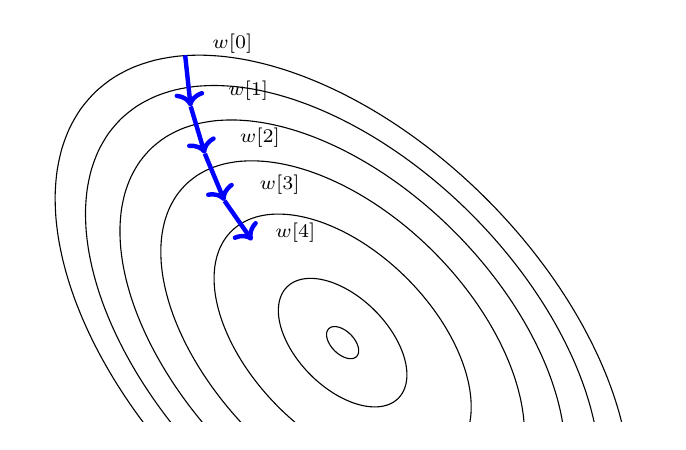
\begin{tikzpicture}[samples=100,smooth]
    \begin{scope}
        \clip(-4,-1) rectangle (4,4);
        \draw plot[domain=0:360] ({cos(\x)*sqrt(20/(sin(2*\x)+2))},{sin(\x)*sqrt(20/(sin(2*\x)+2))});
        \draw plot[domain=0:360] ({cos(\x)*sqrt(16/(sin(2*\x)+2))},{sin(\x)*sqrt(16/(sin(2*\x)+2))});
        \draw plot[domain=0:360] ({cos(\x)*sqrt(12/(sin(2*\x)+2))},{sin(\x)*sqrt(12/(sin(2*\x)+2))});
        \draw plot[domain=0:360] ({cos(\x)*sqrt(8/(sin(2*\x)+2))},{sin(\x)*sqrt(8/(sin(2*\x)+2))});
        \draw plot[domain=0:360] ({cos(\x)*sqrt(4/(sin(2*\x)+2))},{sin(\x)*sqrt(4/(sin(2*\x)+2))});
        \draw plot[domain=0:360] ({cos(\x)*sqrt(1/(sin(2*\x)+2))},{sin(\x)*sqrt(1/(sin(2*\x)+2))});
        \draw plot[domain=0:360] ({cos(\x)*sqrt(0.0625/(sin(2*\x)+2))},{sin(\x)*sqrt(0.0625/(sin(2*\x)+2))});

        \draw[->,blue,ultra thick] (-2,3.65) to (-1.93,3);
        \draw[->,blue,ultra thick] (-1.93,3) to (-1.75,2.4);
        \draw[->,blue,ultra thick] (-1.75,2.4) to (-1.5,1.8);
        \draw[->,blue,ultra thick] (-1.5,1.8) to (-1.15,1.3);

        \node at (-1.4,3.8){\scriptsize $w[0]$};
        \node at (-1.2,3.2){\scriptsize $w[1]$};
        \node at (-1.05,2.6){\scriptsize $w[2]$};
        \node at (-0.8,2){\scriptsize $w[3]$};
        \node at (-0.6,1.4){\scriptsize $w[4]$};
    \end{scope}
\end{tikzpicture}

    \caption{Gradient based learning}
    \label{fig:gradient-descent}
\end{figure}


\begin{figure}[htp]
    \centering
    

% \pgfplotsset{compat=1.17}
% \usetikzlibrary{decorations.pathreplacing}
% \usepackage{pgfplots}

\tikzset{arrowed/.style={decorate,

decoration={show path construction,
moveto code={},
lineto code={
    \draw[#1] (\tikzinputsegmentfirst) --  (\tikzinputsegmentlast);
},
curveto code={},
closepath code={},
}},arrowed/.default={-stealth}}
\pgfplotsset{gradient function/.initial=f,
    dx/.initial=0.01,dy/.initial=0.01}
\pgfmathdeclarefunction{xgrad}{2}{%
    \begingroup%
    \pgfkeys{/pgf/fpu,/pgf/fpu/output format=fixed}%
    \edef\myfun{\pgfkeysvalueof{/pgfplots/gradient function}}%
    \pgfmathparse{(\myfun(#1+\pgfkeysvalueof{/pgfplots/dx},#2)%
    -\myfun(#1,#2))/\pgfkeysvalueof{/pgfplots/dx}}%
    % \pgfmathsetmacro{\mysum}{\mysum+\myfun(\value{isum},#2)}%
    \pgfmathsmuggle\pgfmathresult\endgroup%
}%
\pgfmathdeclarefunction{ygrad}{2}{%
    \begingroup%
    \pgfkeys{/pgf/fpu,/pgf/fpu/output format=fixed}%
    \edef\myfun{\pgfkeysvalueof{/pgfplots/gradient function}}%
    \pgfmathparse{(\myfun(#1,#2+\pgfkeysvalueof{/pgfplots/dy})%
    -\myfun(#1,#2))/\pgfkeysvalueof{/pgfplots/dy}}%
    % \pgfmathsetmacro{\mysum}{\mysum+\myfun(\value{isum},#2)}%
    \pgfmathsmuggle\pgfmathresult\endgroup%
}%

\begin{tikzpicture}
    \begin{axis}
        [width=12cm,%
        declare function={f(\x,\y)=cos(deg(\x)*0.8)*cos(deg(\y)*0.6)*exp(0.1*\x);}]
        \addplot3[surf,shader=interp,domain=-4:4,%samples=81
        ]{f(x,y)};
        \edef\myx{0.15} % first x coordinate
        \edef\myy{-0.15} % first y coordinate
        \edef\mystep{-2}% negative values mean descending
        \pgfmathsetmacro{\myf}{f(\myx,\myy)}
        \edef\lstCoords{(\myx,\myy,\myf)}
        \pgfplotsforeachungrouped\X in{0,...,5}
            {
            \pgfmathsetmacro{\myx}{\myx+\mystep*xgrad(\myx,\myy)}
            \pgfmathsetmacro{\myy}{\myy+\mystep*ygrad(\myx,\myy)}
            \pgfmathsetmacro{\myf}{f(\myx,\myy)}
            \edef\lstCoords{\lstCoords\space (\myx,\myy,\myf)}
        }
        \addplot3[samples y=0,arrowed] coordinates \lstCoords;
    \end{axis}
\end{tikzpicture}
    \caption{Gradient based learning}
    \label{fig:gradient-descent}
\end{figure}

\subsection{Universal Approximation Properties and Depth}
%%%%%%%%%%%%%%%%%%%%%%%%%%%%%%%%%%%%%%%%%%%%%%%%%%%%%%%%%%%%%%%%%%%%%%%%%%%%%%%%

A linear model by definition, may only optimised to represent linear functions.
It has advantages in its simplicity to optimise however we often require our
estimator models to learn nonlinear functions.

%\subsection{Backpropagation}
%%%%%%%%%%%%%%%%%%%%%%%%%%%%%%%%%%%%%%%%%%%%%%%%%%%%%%%%%%%%%%%%%%%%%%%%%%%%%%%%

\newpage{}


\section{Reinforcement Learning\label{ssec:RL}}
%%%%%%%%%%%%%%%%%%%%%%%%%%%%%%%%%%%%%%%%%%%%%%%%%%%%%%%%%%%%%%%%%%%%%%%%%%%%%%%%

\subsection{Key Concepts in Reinforcement Learning}

\subsubsection{Markov Decision Processes (MDP)}

So far, we’ve discussed the agent’s environment in an informal way, but if you
try to go digging through the literature, you’re likely to run into the standard
mathematical formalism for this setting: Markov Decision Processes (MDPs). An
MDP is a 5-tuple, \langle S, A, R, P, \rho_0 \rangle, where

S is the set of all valid states,
A is the set of all valid actions,
R : $S \times A \times S \to \mathbb{R}$ is the reward function, with $r_t = R(s_t, a_t, s_{t+1})$,
P : $S \times A \to \mathcal{P}(S)$ is the transition probability function, with
$P(s'|s,a)$ being the probability of transitioning into state $s'$ if you start
in state $s$ and take action $a$,
and $\rho_0$ is the starting state distribution.

The name Markov Decision Process refers to the fact that the system obeys the
Markov property: transitions only depend on the most recent state and action,
and no prior history.

\tikzset{basic/.style={draw,text width=1em,text badly centered}}
\tikzset{component/.style={rectangle, draw=black, thick, text width=7em,align=center, rounded corners, minimum height=2em}}

\begin{figure}[!htp]
    \centering
    \captionsetup{format=hang} % hanging captions

    \tikzstyle{block} = [rectangle, draw,
    text width=8em, text centered, rounded corners, minimum height=4em]

    \tikzstyle{line} = [draw, -latex]

    \begin{tikzpicture}[node distance = 6em, auto, thick]
        \node [block] (Agent) {Agent};
        \node [block, below=5em of Agent] (Environment) {Environment};
        \node [left=3em of Environment] (Dashed) {};
        \node [above=1.7em of Dashed] (Dashed-up) {};
        \node [below=1.7em of Dashed] (Dashed-down) {};

        \path [line] (Agent.0) --++ (4em,0em) |- node [near start]{Action, $a_t$} (Environment.0);

        \path [line] (Environment.190) -- (Environment.190-|Dashed-down.east) node [midway, label={[xshift=-0.0em]center:$s_{t+1}$}] {\phantom{$s_{t+1}$}};
        \path [line] (Environment.170) -- (Environment.170-|Dashed-up.east) node [midway, above, label={[xshift=-0.0em]center:$r_{t+1}$}] {\phantom{$r_{t+1}$}};

        \path [line] (Environment.190|-Environment.190) --++ (-6em,0em) |- node [near start] {} node [near start, label={[xshift=-0.0em]center:State, $s_t$}] {\phantom{State, $s_t$}} (Agent.170);
        \path [line] (Environment.170|-Environment.170) --++ (-4.25em,0em) |- node [near start, right] {} node [near start, right, label={[xshift=-0.0em]center:Reward, $r_t$}] {\phantom{Reward, $r_t$}} (Agent.190);

        \draw[dotted] (Dashed-up.east) -- (Dashed-down.east);


    \end{tikzpicture}
    \caption{\textbf{The agent-environment interaction interface} illustrates the interaction between an agent and its environment. The agent takes an action $a_t$ and receives a reward $r_{t+1}$ and a new state $s_{t+1}$, subject to the environment's dynamics.}
    \label{fig:agent-environment}

\end{figure}

\begin{itemize}
    \item states and observations,
    \item action spaces,
    \item policies,
    \item trajectories,
    \item different formulations of return,
    \item the RL optimization problem,
    \item and value functions.
\end{itemize}

\subsection{Taxonomy of Reinforcement Learning}
%%%%%%%%%%%%%%%%%%%%%%%%%%%%%%%%%%%%%%%%%%%%%%%%%%%%%%%%%%%%%%%%%%%%%%%%%%%%%%%%

\subsection{Value-based methods}
%%%%%%%%%%%%%%%%%%%%%%%%%%%%%%%%%%%%%%%%%%%%%%%%%%%%%%%%%%%%%%%%%%%%%%%%%%%%%%%%

\subsection{Policy-based methods}
%%%%%%%%%%%%%%%%%%%%%%%%%%%%%%%%%%%%%%%%%%%%%%%%%%%%%%%%%%%%%%%%%%%%%%%%%%%%%%%%

\subsection{Policy gradient}
%%%%%%%%%%%%%%%%%%%%%%%%%%%%%%%%%%%%%%%%%%%%%%%%%%%%%%%%%%%%%%%%%%%%%%%%%%%%%%%%

\subsection{Deep deterministic policy gradient (DDPG)}
%%%%%%%%%%%%%%%%%%%%%%%%%%%%%%%%%%%%%%%%%%%%%%%%%%%%%%%%%%%%%%%%%%%%%%%%%%%%%%%%


    \newpage
    
    \printbibliography

    \backmatter

    \appendix
%    \begin{appendices}
    %%%%%%%%%%%%%%%%%%%%%%%%%%%%%%%%%%%%%%%%%%%%%%%%%%%%%%%%%%%%%%%%%%%%%%%%%%%%%%%%
\section{Mathematical Expressions\label{app:a}}
%%%%%%%%%%%%%%%%%%%%%%%%%%%%%%%%%%%%%%%%%%%%%%%%%%%%%%%%%%%%%%%%%%%%%%%%%%%%%%%%

%%%%%%%%%%%%%%%%%%%%%%%%%%%%%%%%%%%%%%%%%%%%%%%%%%%%%%%%%%%%%%%%%%%%%%%%%%%%%%%%

\subsection{Rotation transformations\label{appendix:rotational_transformations}}
%%%%%%%%%%%%%%%%%%%%%%%%%%%%%%%%%%%%%%%%%%%%%%%%%%%%%%%%%%%%%%%%%%%%%%%%%%%%%%%%

\begin{equation}
    \mathbb{T}_x(\phi_x)=
    \begin{bmatrix}
        1 & 0           & 0          \\
        0 & \cos\phi_x  & \sin\phi_x \\
        0 & -\sin\phi_x & \cos\phi_x \\
    \end{bmatrix}
\end{equation}

\begin{equation}
    \mathbb{T}_y(\phi_y)=
    \begin{bmatrix}
        \cos\phi_y  & 0 & -\sin\phi_y \\
        0           & 1 & 0           \\
        -\sin\phi_y & 0 & \cos\phi_y  \\
    \end{bmatrix}
\end{equation}

\begin{equation}
    \mathbb{T}_z(\phi_z)=
    \begin{bmatrix}
        \cos\phi_z  & \sin\phi_z & 0 \\
        -\sin\phi_z & \cos\phi_z & 0 \\
        0           & 0          & 1 \\
    \end{bmatrix}
\end{equation}

%%%%%%%%%%%%%%%%%%%%%%%%%%%%%%%%%%%%%%%%%%%%%%%%%%%%%%%%%%%%%%%%%%%%%%%%%%%%%%%%

\subsection{Incomplete integrals\label{appendix:incomplete_integrals}}
%%%%%%%%%%%%%%%%%%%%%%%%%%%%%%%%%%%%%%%%%%%%%%%%%%%%%%%%%%%%%%%%%%%%%%%%%%%%%%%%

\begin{equation}
    U(r_x, r_y, r_z) = G\int_V\frac{\rho{(s_x,s_y,s_z)}}{\sqrt{(r_x-s_x)^2+(r_y-s_y)^2+(r_z-s_z)^2}}\;dx\;dy\;dz
    \label{eq:ur-gen-rect}
\end{equation}

\begin{equation}
    R_F\!\left(x, y, z\right) = \frac{1}{2} \int_{0}^{\infty} \frac{1}{\sqrt{t + x} \sqrt{t + y} \sqrt{t + z}} \, dt
    \label{eq:elliptic_RF}
\end{equation}

\begin{equation}
    R_D\!\left(x, y, z\right) = \frac{3}{2} \int_{0}^{\infty} \frac{1}{\left(t + x\right) \left(t + y\right) {\left(t + z\right)}^{3 / 2}} \, dt
    \label{eq:elliptic_RD}
\end{equation}


%%%%%%%%%%%%%%%%%%%%%%%%%%%%%%%%%%%%%%%%%%%%%%%%%%%%%%%%%%%%%%%%%%%%%%%%%%%%%%%%

\subsection{Vector norms\label{appendix:vector_norms}}
%%%%%%%%%%%%%%%%%%%%%%%%%%%%%%%%%%%%%%%%%%%%%%%%%%%%%%%%%%%%%%%%%%%%%%%%%%%%%%%%
Given $x\in\gls{set:R}^n$, the vector norms for $\ell_p(\mathbf{x})$ are defined
by the following equations:

\begin{equation}
    \ell_1(\mathbf{x})=||\mathbf{x}||_1 = \sum_{d=1}^n |x_d|
\end{equation}

\begin{equation}
    \ell_2(\mathbf{x})=||\mathbf{x}||_2 = \sqrt{\sum_{d=1}^n x_d^2}
\end{equation}

\begin{equation}
    \ell_\infty(\mathbf{x})=||\mathbf{x}||_\infty = \max_{1\leq{d}\leq{n}}^n |x_d|
\end{equation}

\begin{equation}
    \ell_p(\mathbf{x})=||\mathbf{x}||_p=
    \begin{cases}
        \bigg(\sum_{d=1}^n |x_d|^p\bigg)^{1/p}    &  1\leq{}p\le \infty \\
        \max_{1\leq{d}\leq{n}}^n |x_d|            &  p=\infty \\
    \end{cases}
    \label{eq:ell-p}
\end{equation}


    %%%%%%%%%%%%%%%%%%%%%%%%%%%%%%%%%%%%%%%%%%%%%%%%%%%%%%%%%%%%%%%%%%%%%%%%%%%%%%%%
\newpage\section*{Appendix B: Orbital Mechanics}
%%%%%%%%%%%%%%%%%%%%%%%%%%%%%%%%%%%%%%%%%%%%%%%%%%%%%%%%%%%%%%%%%%%%%%%%%%%%%%%%

%%%%%%%%%%%%%%%%%%%%%%%%%%%%%%%%%%%%%%%%%%%%%%%%%%%%%%%%%%%%%%%%%%%%%%%%%%%%%%%%
\subsection*{Conversions of Orbital Elements}
%%%%%%%%%%%%%%%%%%%%%%%%%%%%%%%%%%%%%%%%%%%%%%%%%%%%%%%%%%%%%%%%%%%%%%%%%%%%%%%%

%%%%%%%%%%%%%%%%%%%%%%%%%%%%%%%%%%%%%%%%%%%%%%%%%%%%%%%%%%%%%%%%%%%%%%%%%%%%%%%%
\subsubsection*{Modified Equinoctial to Keplerian\label{mee2kep}}
%%%%%%%%%%%%%%%%%%%%%%%%%%%%%%%%%%%%%%%%%%%%%%%%%%%%%%%%%%%%%%%%%%%%%%%%%%%%%%%%

\begin{equation}
    a = \frac{p}{1-f^2-g^2}
\end{equation}

\begin{equation}
    e = \sqrt{f^2 + g^2}
\end{equation}

\begin{equation}
    i = 2\tan^{-1}{\sqrt{h^2+k^2}}=\textrm{atan2}(2\sqrt{h^2+k^2},1-h^2-k^2)
\end{equation}

\begin{equation}
    i = 2\tan^{-1}{\sqrt{h^2+k^2}}=\textrm{atan2}(2\sqrt{h^2+k^2},1-h^2-k^2)
\end{equation}

\begin{equation}
    \omega=\tan^{-1}(g/f)-\tan^{-1}(k/h)=\textrm{atan2}(gh-fk, fh+gk)
\end{equation}

\begin{equation}
    \Omega=\textrm{atan2}(k, h)
\end{equation}

\begin{equation}
    \theta = L-(\Omega+\omega)=L-\tan^{-1}(g/f)
\end{equation}

\begin{equation}
    u = \omega+\theta = \textrm{atan2}(h\sin{L}-k\cos{L},h\cos{L}+k\sin{L})
\end{equation}

%%%%%%%%%%%%%%%%%%%%%%%%%%%%%%%%%%%%%%%%%%%%%%%%%%%%%%%%%%%%%%%%%%%%%%%%%%%%%%%%
\subsubsection*{Modified Equinoctial to Cartesian\label{mee2rec}}
%%%%%%%%%%%%%%%%%%%%%%%%%%%%%%%%%%%%%%%%%%%%%%%%%%%%%%%%%%%%%%%%%%%%%%%%%%%%%%%%

%%%%%%%%%%%%%%%%%%%%%%%%%%%%%%%%%%%%%%%%%%%%%%%%%%%%%%%%%%%%%%%%%%%%%%%%%%%%%%%%
\subsubsection*{Cartesian to Modified Equinoctial\label{rec2mee}}
%%%%%%%%%%%%%%%%%%%%%%%%%%%%%%%%%%%%%%%%%%%%%%%%%%%%%%%%%%%%%%%%%%%%%%%%%%%%%%%%

%%%%%%%%%%%%%%%%%%%%%%%%%%%%%%%%%%%%%%%%%%%%%%%%%%%%%%%%%%%%%%%%%%%%%%%%%%%%%%%%
\subsubsection*{Keplerian to Cartesian\label{kep2rec}}
%%%%%%%%%%%%%%%%%%%%%%%%%%%%%%%%%%%%%%%%%%%%%%%%%%%%%%%%%%%%%%%%%%%%%%%%%%%%%%%%

%%%%%%%%%%%%%%%%%%%%%%%%%%%%%%%%%%%%%%%%%%%%%%%%%%%%%%%%%%%%%%%%%%%%%%%%%%%%%%%%
\subsubsection*{Cartesian to Keplerian\label{rec2kep}}
%%%%%%%%%%%%%%%%%%%%%%%%%%%%%%%%%%%%%%%%%%%%%%%%%%%%%%%%%%%%%%%%%%%%%%%%%%%%%%%%


%    \end{appendices}

\end{document}